\documentclass[a4paper,12pt,twoside]{article}
\usepackage{graphicx}
\graphicspath{ {./images/} }
\usepackage{wrapfig}
%\usepackage{indentfirst} % Uncomment to indent first paragraph of each section (not really correct for academic papers, but follows more common business convention)
\usepackage{pdfpages,caption,geometry} %enables you to add pdf and a caption

\usepackage{geometry}
\geometry{
  a4paper,
  total={170mm,257mm},
  left=20mm,
  top=40mm,
  bottom=30mm,
}

\usepackage{fontspec}
\setmainfont{Exo 2}[%
    Path            =   fonts/,
    Extension       =   .otf,
    UprightFont     =   *-Regular,
    ItalicFont      =   *-Italic,
    BoldFont        =   *-Bold,
    BoldItalicFont  =   *-BoldItalic,
    FontFace        =   {black}{n}{*-Black},
    FontFace        =   {black}{it}{*-BlackItalic},
]

\usepackage[dvipsnames]{xcolor}
\definecolor{RHgrey}{RGB}{101,101,101}
\definecolor{RHblue}{RGB}{7,163,216}
\definecolor{RHgreen}{RGB}{30,165,43}
\definecolor{RHyellow}{RGB}{251,210,0}
\definecolor{code}{RGB}{200,200,200}
\definecolor{textbox}{RGB}{200,255,200}
\definecolor{captiongreen}{RGB}{50,165,60}
  
\usepackage{sectsty}
\sectionfont{\color{RHblue}} 
\subsectionfont{\color{RHblue}}
\subsubsectionfont{\color{RHblue}}

\usepackage{caption}
\usepackage[font={color=captiongreen,small,bf},figurename=Fig.,labelfont={small,it}]{caption}
\usepackage{subcaption} 

\usepackage[utf8]{inputenc}
\usepackage[english]{babel}

\usepackage{multicol} % Allows multiple columns to be used on the fly

\usepackage{fancyhdr}
\pagestyle{fancy}
\fancyhf{}
\lhead{\color{RHgrey} \leftmark}
\rhead{\color{RHgrey} \rightmark}
\fancyfoot[LE]{\color{RHgrey} \thepage \hspace{5mm} \scriptsize RAMANI HURIA INTERIM REPORT 4}
\fancyfoot[RO]{\color{RHgrey} \scriptsize RAMANI HURIA INTERIM REPORT 4 \hspace{3mm} \normalsize \thepage}

\usepackage{hyperref}
\hypersetup{
  colorlinks=true,
  linkcolor=RHblue, % to match the Ramani Huria blue text
  filecolor=magenta,      
  urlcolor=cyan,
  pdftitle={RH Interim Report 4},
  %pdfpagemode=FullScreen,
}
%\urlstyle{same}

\usepackage[framemethod=tikz]{mdframed}
\usepackage{lipsum}


\title{Ramani Huria Interim Report 4}
\author{Humanitarian OpenStreetMap Team}
\usepackage[nodayofweek,level]{datetime}
\newdate{date}{15}{04}{2019}
\date{\displaydate{date}}

\newcommand*{\vcenteredhbox}[1]{\begingroup
\setbox0=\hbox{#1}\parbox{\wd0}{\box0}\endgroup} % For creating vertically centered rows of logos

\setcounter{tocdepth}{2} % Table of Contents includes only sections and subsections, not subsubsections.

\begin{document}
\thispagestyle{empty}
\begin{center}
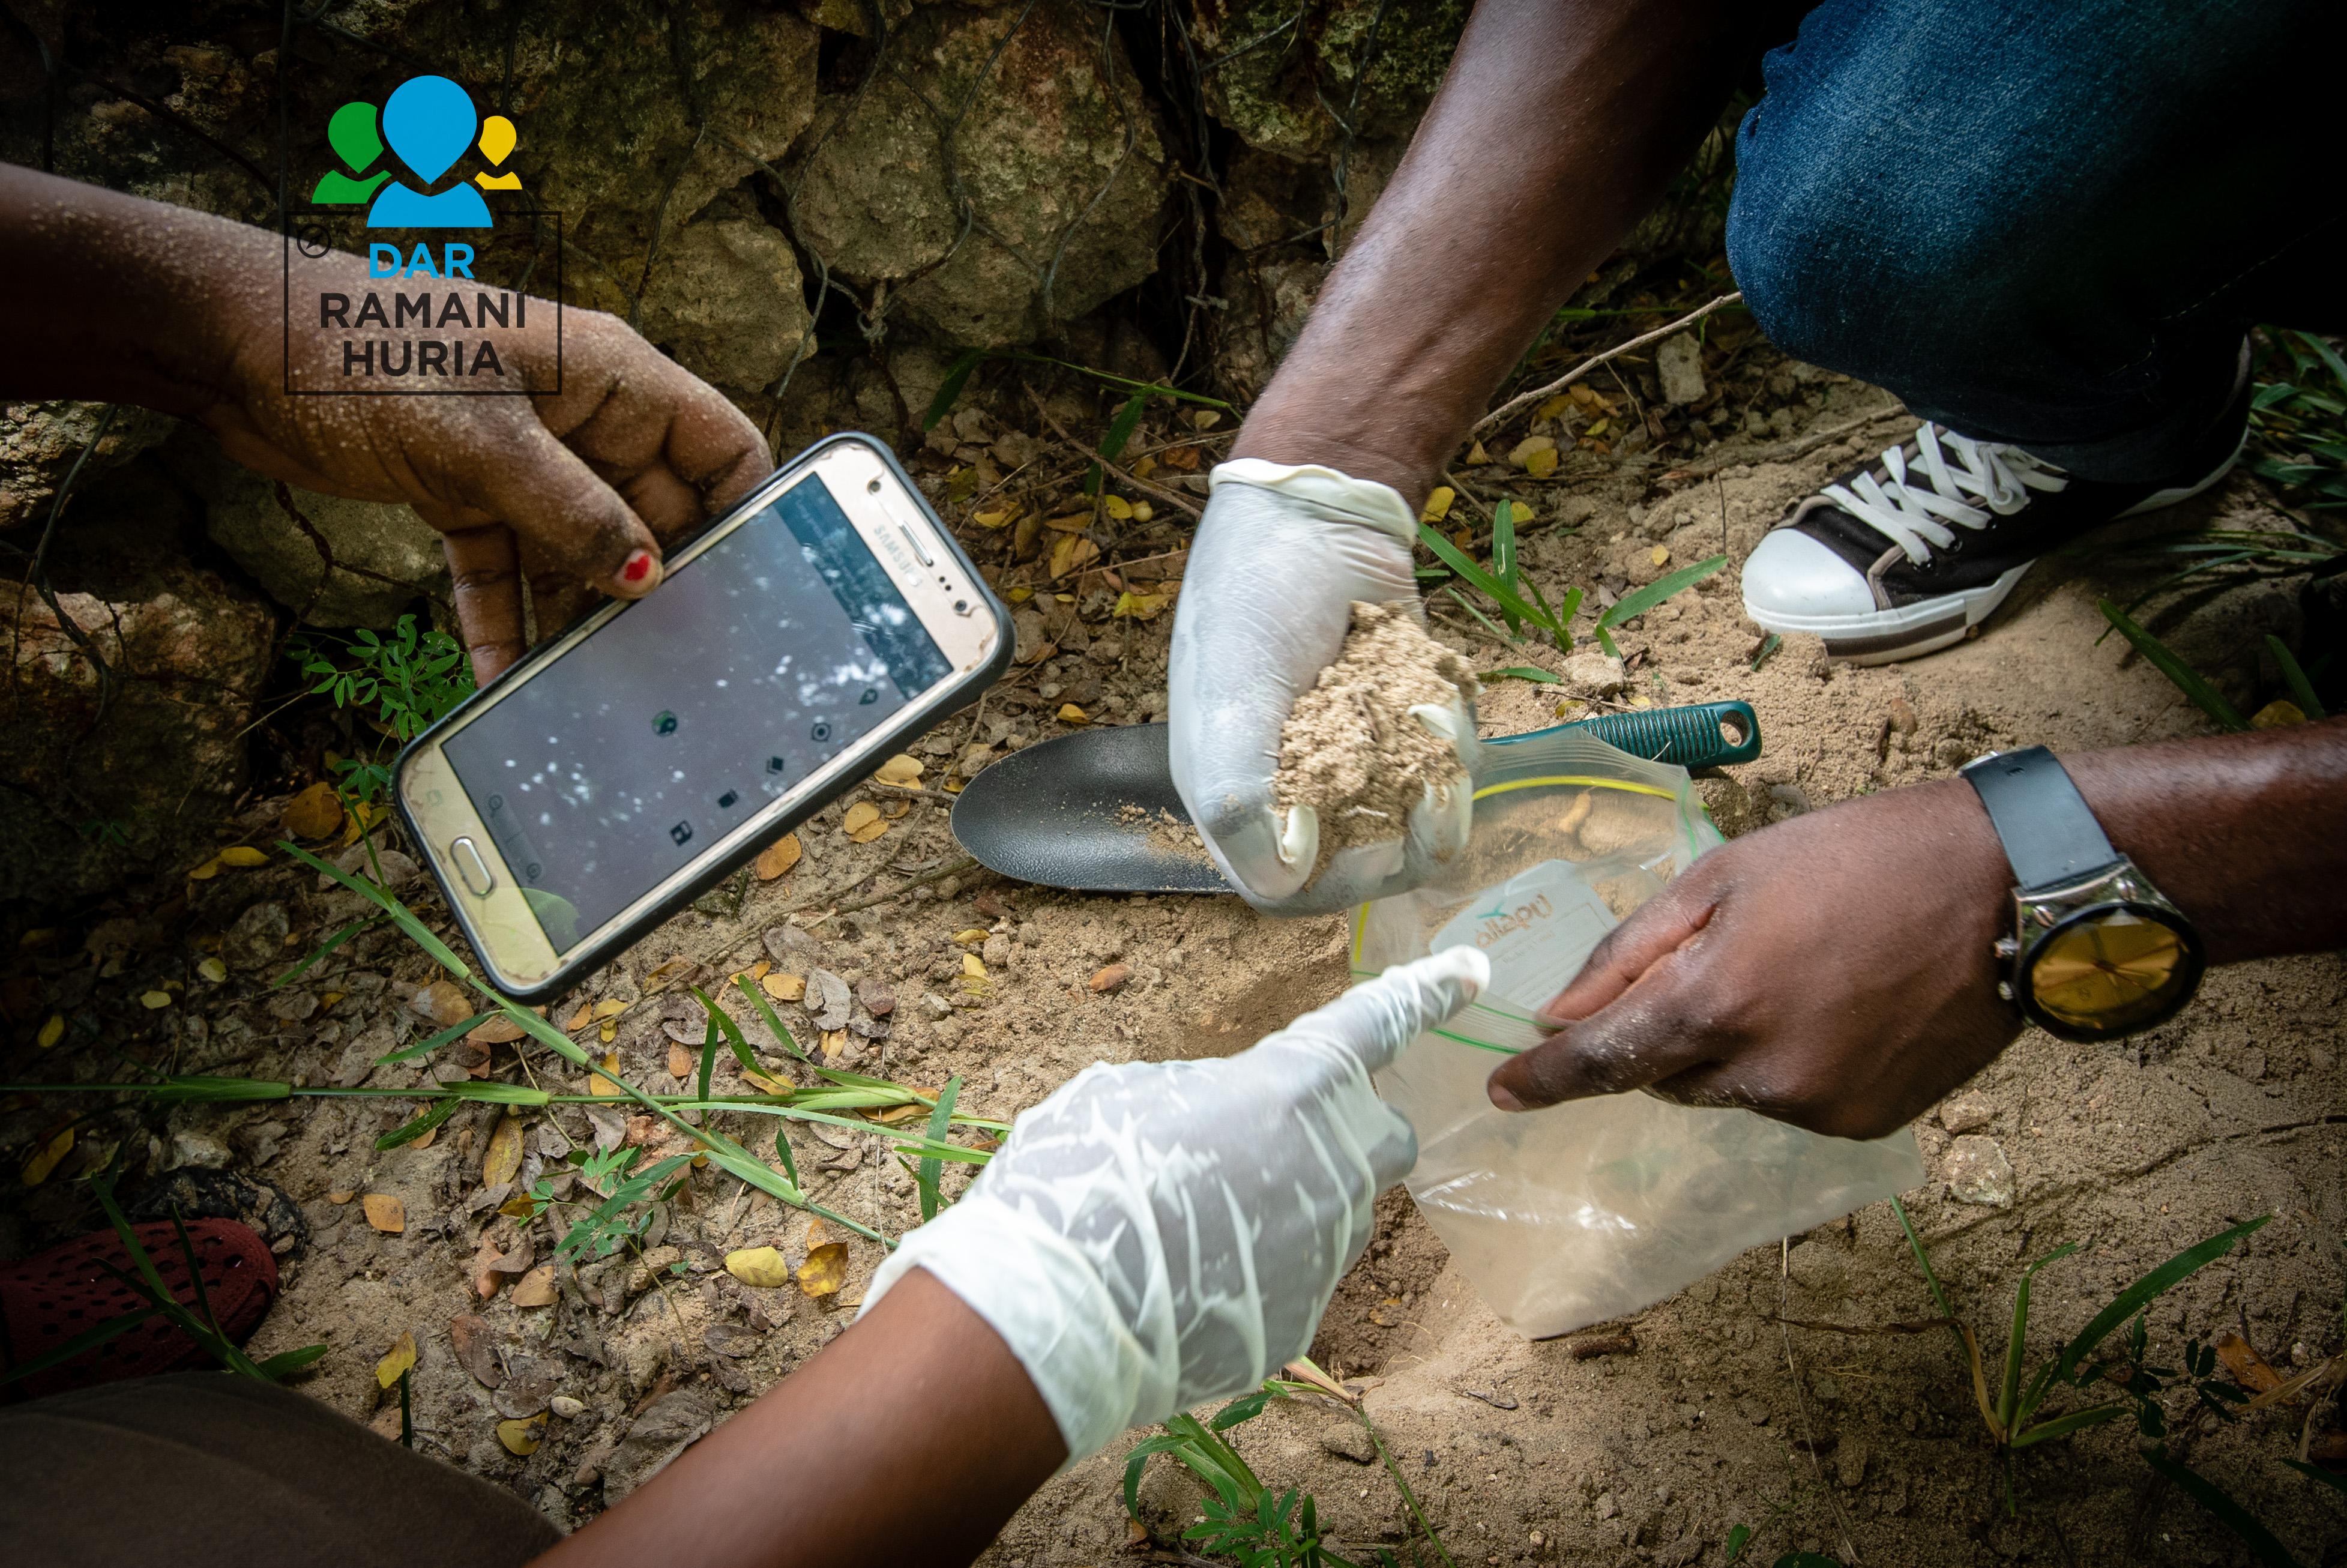
\includegraphics[width=\textwidth]{Cover_photo_with_logo.jpg}
\end{center}
\bigskip
\begin{center}
  \Huge \color{RHblue} \textbf {RAMANI HURIA}

\textbf{INTERIM REPORT 4}
\end{center}
\bigskip
\vbox{
  \centering
  Prepared for:
  \vcenteredhbox{
\includegraphics[width=2cm]{UK-aid_logo.png}}
  and { }
  \vcenteredhbox{
\includegraphics[width=7cm]{images/World_Bank_Group_logo.png}}
  \
  
  by:
  \vcenteredhbox{
\includegraphics[width=4cm]{HOT_logo_with_text.png}}
  % \maketitle
  
}
\medskip
\begin{center}
  Humanitarian OpenStreetMap
  \
  
  15 April, 2019
\end{center}
\bigskip
\bigskip
\bigskip
\begin{center}
\color{RHblue}\rule{\textwidth}{0.6cm}
\end{center}

\newpage
\color{RHgrey}

\begin{center}
{
\includegraphics[width=5cm]{Dar_Ramani_Huria_logo.png}}
\end{center}

This report was prepared by William Evans, Immaculate Mwanja, Hawa Adinani, Innocent Maholi, Ivan Buendia Gayton, and many others from the Humanitarian OpenStreetMap Team in Tanzania.

\medskip

Graphic design by Ivan Buendia Gayton and Immaculate Mwanja based on the Ramani Huria design guideline by Darragh Amelia Coward. Layout was done using the \LaTeX { } typesetting system.

\medskip

Guidance and input on the project came from Edward Anderson, Caroline Gevaert, Roza Vasileva, and Msilikale Msilanga at the World Bank.

\medskip

Unless otherwise noted, photos by the Ramani Huria team. Maps were prepared by the Ramani Huria team using QGIS.

\bigskip\bigskip\bigskip\bigskip\bigskip

\vcenteredhbox{
\includegraphics[height=2cm]{images/logo_Coat_of_arms_of_Tanzania.png}}
\vcenteredhbox{
\includegraphics[height=2.2cm]{UK-aid_logo.png}}
\vcenteredhbox{
\includegraphics[height=1.2cm]{images/World_Bank_Group_logo.png}}
\vcenteredhbox{
\includegraphics[height=0.7cm]{images/logo_GFDRR.png}}

\medskip

\vcenteredhbox{
\includegraphics[height=1.2cm]{images/logo_dar-es-salaam.jpg}}
\vcenteredhbox{
\includegraphics[height=1.2cm]{images/logo_Ardhi.png}}
\vcenteredhbox{
\includegraphics[height=1.2cm]{images/logo_costech.png}}
\vcenteredhbox{
\includegraphics[height=1.2cm]{images/logo_UDSM.jpg}}


\newpage
{\color{RHblue}\LARGE{Licensing}}
\begin{itemize}
    \item
    \href{https://creativecommons.org/licenses/by/4.0/}{Creative Commons (CC-BY 4.0)}\footnote{\url{https://creativecommons.org/licenses/by/4.0/}}
This is a public copyright license that enables the free distribution of an otherwise copyrighted work. A CC license is used when an author wants to give other people the right to share, use, and build upon a work that he or she has created. Most of the Ramani Huria data use a public copyright license to enable users to share and use the data freely.
\item 
\href{https://en.wikipedia.org/wiki/Open_Database_License}{Open Data Commons Open Database License (ODbL)}\footnote{\url{https://en.wikipedia.org/wiki/Open_Database_License}}.
The ODbL was created with the goal of allowing users to share their data freely without worrying about problems relating to copyright or ownership. It allows users to make free use of the data in the database without worrying about copyright of the creators, and add to the data or use in other databases. The license establishes the rights of users of the database, as well as the correct procedure for attributing credit where credit is due for the data, and how to make changes or improvements in the data, thus simplifying the sharing and comparison of data. Users no longer need to worry of repercussions of violations of copyright law or stolen information when using an Open Database License.

\end{itemize}
\bigskip

{\color{RHblue}\LARGE{Data Model}}\bigskip

Only data that have been uploaded to OpenStreetMap have a clear defined data model, So for data with no defined data modle will be linked to ODK survey questions that was used to collect them or linked to the wikipage that clarify how that dataset was obtained.
\newpage

\tableofcontents
\newpage
\section{Executive Summary}
\label{executivesummary}
\begin{multicols}{2}

 
    
With the support of the World Bank in Tanzania, the Ramani Huria (RH) team has been collecting data for urban resilience with a particular emphasis on flooding since 2015. As the program nears its end in September of 2019, the RH team is now primarily working to curate, organize, document, and publish the data, tools and knowledge that have been created. 

We are working to transfer knowledge and hand over to Tanzania Resilience Academy, the successor project to Ramani Huria. 


Together with the coalescing Resilience Academy team, we are working to disseminate the knowledge and data to as many users---particularly those who are likely to have impact improving resilience---as possible. 

%I want this report to get 100\% marks

Ramani Huria 2.0 is next to last in June 2019, During this phase we have collected a number of datasets that can serve for different purposes. 
Data set collected include; Soil sediment sampling, Drainage mapping, Flood extent data, Hyperlocal boundaries mapping, Threat and asset mapping (Flood risks identification), Trash mapping for waste management, Flood response mapping (damage assessment) and buildings footprint digitization.

This overview of digital datasets is meant to be used as an annex to the final report on June 2019. It contains a brief summary of the dataset, spatial extent, methodology used for data collection, data model and/or survey form used, Methods used to ensure data quality, data gap, timeline, statistics, visualization of data, link to access data, Licencing (incase of sharing), data use case and lessons learned throughout the process of data collection.

Ramani Huria team conducted a number of activities including Community flood response following the heavy rainfall on March 3rd 2019, Soil sediment analysis for geomorphological assessment of the city and erosion modeling, Participated in Innovation week on March 2019 to showcase how we conducted sediment analysis using cheap yet practical method and came out with professional results and The ongoing River mapping activity --flying drones along major rivers of dar es salaam to  provide a digital photographic mark-up of the current status of Dar es Salaam’s waterways, to help in solid waste management on major rivers of the city.


\end{multicols}

%\includegraphics[width=0.8\textwidth]{sample_locations.jpg}

\newpage
\section{Introduction}
\label{Introduction}

This report will tell you about stuff

\begin{itemize}
  \item Like this
  \item And this
\end{itemize}

We also would like to point out a link to  \href{https://ramanihuria.org}{a website}\footnote{\url{http://ramanihuria.org}\color{RHgrey} { }because it's really, really interesting. You should click on that link.}. Did you notice that there was a footnote there? If you look at the footnote it contains the full URL of the link, so that people reading the document on paper can see what it links to? Cool, huh? The rest of the text on this page will be in two columns, just because we can do that with the \LaTeX{} \textbf{\textit{multicols}} plugin. By the way, I can highlight code with a color box like \textbf{\colorbox{code}{this.}}

\begin{multicols}{2}

  This report describes the activities of Ramani Huria 2.0 from October to February and provides an overview of digital assets collected since October. 
  
\end{multicols}

\newpage
\section{Monthly Activity Summary}
\subsection{Community Flood Response}
As a response to heavy rainfall on March, 3rd, 2019 which started from 6am to 10 am, that resulted in heavy flooding in some wards of Dar es Salaam, the Ramani Huria team decided to conduct field mapping to engage affected communities with the aim of conducting a rapid assessment and producing impact maps. In the wards we surveyed, a total of 1907 houses were flooded. 
On 5th - 6th March 2019 the Ramani Huria team visited Mkunguni B Subward (Hananasif Ward), Mkunduge Subward and Sokoni Subward (Tandale ward) as well as Mtambani A Subward (Jangwani Ward). These areas were prioritized by first communicating with the local leaders over the phone. The team used their \href{https://docs.google.com/spreadsheets/d/1x8fJiSwX-zM05GCxfd4t1XsQqwRf7Us7V6cQaNlkq8E/edit#gid=0}{contact database}\footnote{\url{https://docs.google.com/spreadsheets/d/1x8fJiSwX-zM05GCxfd4t1XsQqwRf7Us7V6cQaNlkq8E/edit#gid=0}} which contains more than 3000 phone numbers of Subward Executive Officers, Ward Executive Officers, Chairpersons, and local leaders. In order to identify the affected communities, we conducted a community meeting with MEO’s, chairpersons and shina leaders.

\medskip
\href{https://docs.google.com/document/d/1gZR94UHdUNR5646agKCPFX7jrdJKmXhMjetb9MweOJ4/edit#}{Community Flood Response Report}\footnote{\url{https://docs.google.com/document/d/1gZR94UHdUNR5646agKCPFX7jrdJKmXhMjetb9MweOJ4/edit#}}

\medskip
\href{https://drive.google.com/drive/u/0/folders/14Bp8qZxcOSvfb3JlEbHWNRYSeq6JcqmX}{Flood Response Maps}\footnote{\url{https://drive.google.com/drive/u/0/folders/14Bp8qZxcOSvfb3JlEbHWNRYSeq6JcqmX}}
\subsection{Soil Sampling}
With the support of the World Bank in Tanzania, Ramani Huria and JBA Consulting partnered in October 2018 to develop a surface soil sediment dataset for the greater Dar es Salaam region of Tanzania. This was intended to support a geomorphological assessment taking into account soil sediment characteristics for erosion and flood risk studies.
A national-level soil profile had existed for Tanzania prior to this effort but contained only a single sample from Dar es Salaam. This was not sufficient to analyse erosion potential across the city. The JBA team in consultation with Ramani Huria decided to use a 2km grid, which resulted in 731 sampling points being pre-established throughout the city. A team of 10 field mappers and 4 office technicians—all Tanzanian youth participants in the Ramani Huria project—were trained in sample collection and analysis (sieving). A total of 643 points were sampled and sieved; 88 sites were inaccessible for one or another reason.
The 643 samples were analyzed by sieving each to separate the sediment by particle size and weighing the resulting fractions. The resulting dataset, a geo-referenced set of soil sediment profiles, is published and available as \href{https://geonode.uhurulabs.org/layers/geonode3A_2019_02_26_dar_soil_sampling_final_results_v1}{open data}\footnote{\url{https://geonode.uhurulabs.org/layers/geonode3A_2019_02_26_dar_soil_sampling_final_results_v1}}.

\subsection{Innovation Week}
This is a week-long series of events hosted by Human Development Innovation Fund (HDIF) and COSTECH with support from UKAid. This year’s innovation week took place from the 25th - 30th of March with a theme “Scaling and Sustaining Innovation for Human Development”. Ramani Huria team participated by showcasing the soil sediment sampling project that we did using cheap but yet practical methods and came out with sediment characteristics of the whole city.
We also showcased a drone that was built locally using bamboo with the aim of capturing aerial images at a low cost without importing drones, which might be expensive. This also aligns with our slogan of local people, local devices and open knowledge.

\subsection{River Mapping}
Several drone flights have been conducted along five major rivers of Dar es Salaam i.e. Msimbazi, Mpiji, Tegeta, Kizinga and Mzinga Rivers, covering a total length of approximately 60 km of Dar es Salaam’s critical water arteries. The drone flights provide a digital photographic mark-up of the current status of Dar es Salaam’s waterways. The broad purpose of this work is to provide Nipe Fagio, I4ID and other partners with high-quality and interactive spatial data to better understand solid waste management and service quality across all five municipalities of Dar es Salaam and all of the city’s key five rivers.

Drone flights are capable of studying any aggregations of waste/ informal dumps that are on the banks of the river/ waterway or within five metres of its bank on either side. 
Such data will be presented as three-dimensional imagery of waste piles/ aggregations, further assisting the study team to estimate rough waste volumes.


\newpage
\begin{itemize}

\textbf{\item October 2018}    
    \begin{itemize}
        \item Drainage Mapping
        \item Hyper-local administrative boundary mapping
        \item Soil sampling
        \item Tabata Trash Mapping
    \end{itemize}
\textbf{\item November 2018}    
    \begin{itemize}
        \item Hyper-local administrative boundary mapping
        \item Soil sampling
        \item Tabata Trash Mapping
    \end{itemize}
\textbf{\item December 2018}    
    \begin{itemize}
        \item Hyper-local administrative boundary mapping
        \item Soil sampling
        \item Tabata Trash Mapping
        \item Asset and Threat Mapping
        \item Data publication on GeoNode with Uhurulabs
    \end{itemize}
\textbf{\item January 2019}    
    \begin{itemize}
        \item Drainage mapping
        \item Tabata Trash Mapping
        \item Asset and Threat Mapping
    \end{itemize}
\textbf{\item February 2019}
    \begin{itemize}
        \item Soil sampling
        \item Tabata Trash Mapping
        \item Tabata Trash Mapping
        \item Drainage Mapping
        \item Asset and Threat Maps Production
        \item Data Quality Assurance
        \item Data publication on GeoNode with Uhurulabs
    \end{itemize}
\end{itemize}
\newpage
\section{Team Composition and Assignments}
Hi there!
\newpage
\section{Data Quality}
The process of data profiling to discover inconsistencies and other anomalies in the data, as well as performing data cleaning activities (e.g. removing outliers, missing data interpolation) to improve the data quality. Data description is done using descriptive statistics; these are used to describe the basic features of the data in a study. They provide simple summaries about the sample and the measures. Together with simple graphics analysis, they form the basis of virtually every quantitative analysis of data. Data quality activities involve data rationalization and validation.
Ramani Huria data uses a data quality framework as a guide for each dataset to ensure the data is cleaned following certain procedures and steps. The objective of the framework is to provide insight into the Ramani Huria data quality process as well as to guide future projects in best practices. See  \href{https://docs.google.com/document/d/1IE1ARLs6i4d_KTK73X9LGbU2OoEHCgDRefE47J6LJn8/edit#}{Ramani Huria Data Quality Framework}\footnote{\url{https://docs.google.com/document/d/1IE1ARLs6i4d_KTK73X9LGbU2OoEHCgDRefE47J6LJn8/edit#}}



\section{Datasets}
In this case a dataset contain all digital data collected by Ramani Huria from October to February. Not all data can contain all character of a 'dataset' but rather providing an overview of Ramani Huria data collected. The following is a list of datasets all presented in the same format for consistency. 
\subsection{Drainage}
\begin{wrapfigure}{r}{0.25\textwidth} %this figure will be at the right
    \centering
    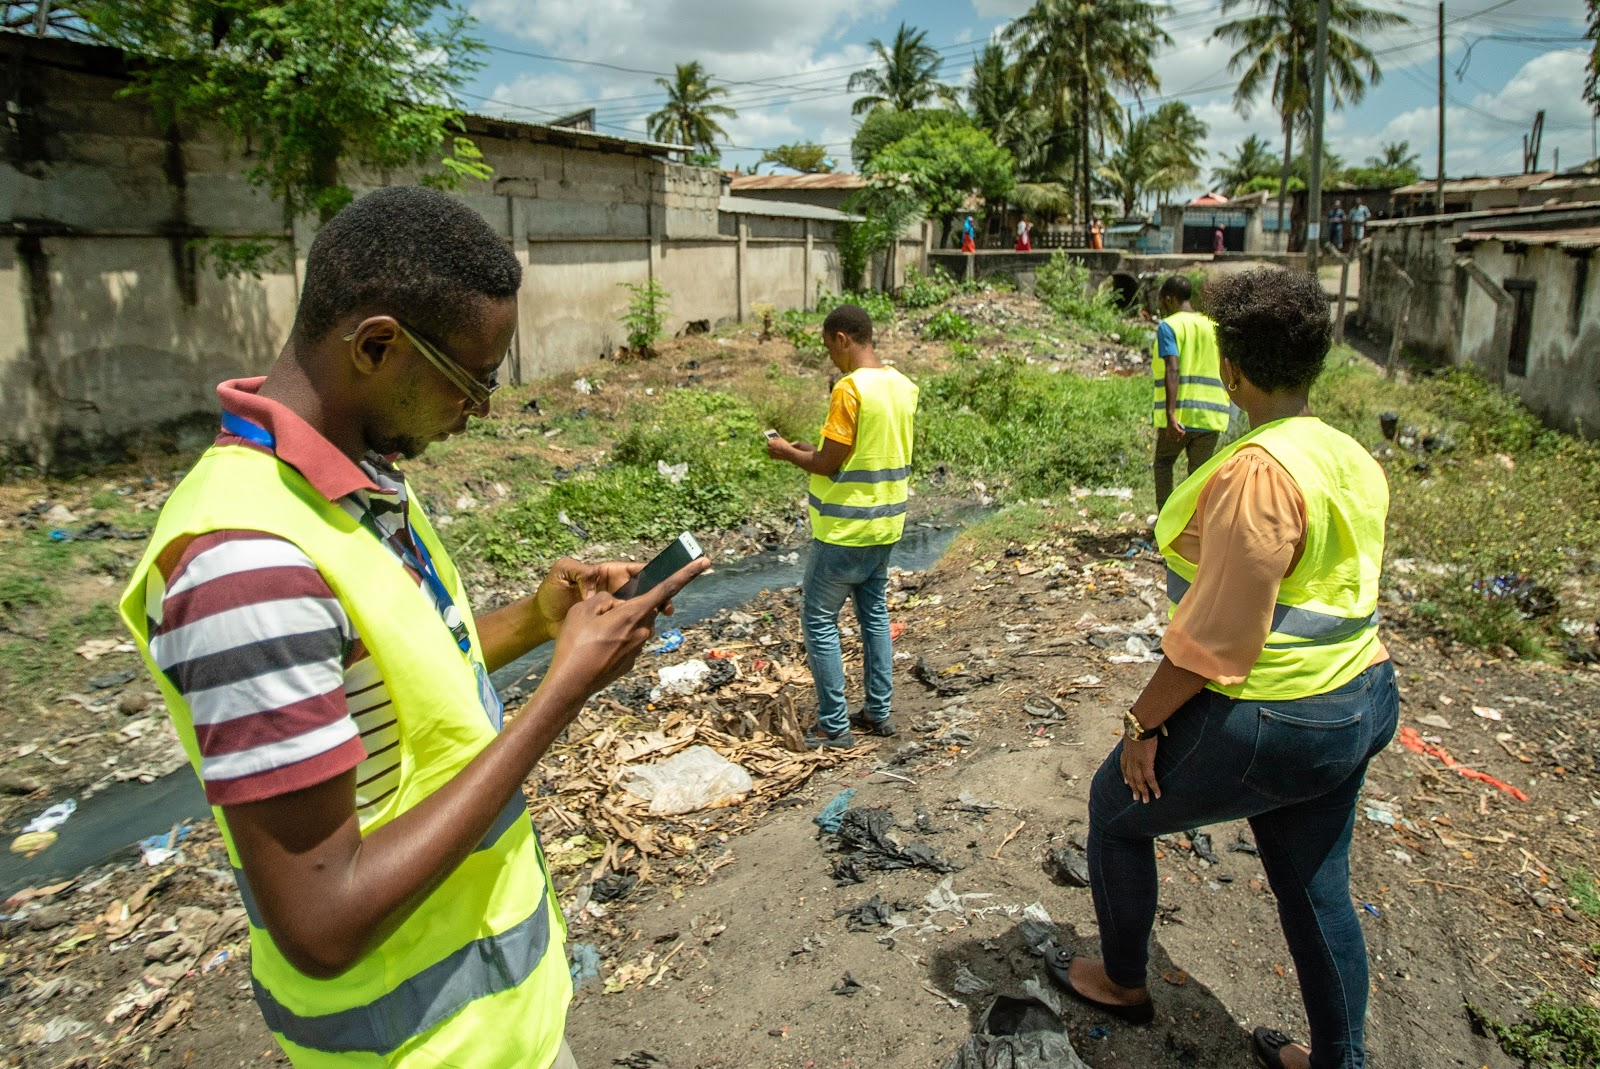
\includegraphics[width=0.25\textwidth]{images/Drainage_Mapping.jpg}
\end{wrapfigure}

\

Drainage data collected in the most flood prone areas across Dar es Salaam using cheap  and practical methods. This information will be used to develop a flood model which requires accurately collected specifications of drains such as depth, width, blockage (by either vegetation or material), connectivity, and diameter (typically for culverts).

\subsubsection{Spatial Extent}
Drainage data covers 44 prioritized Ramani Huria wards most of which are along the Msimbazi and Ng’ombe rivers. Almost 90\% of the wards have been mapped.

\begin{figure}[h]
  \color{RHgreen}\caption{Map showing the drainage mapping progress as of March, 2019}
  \centering
  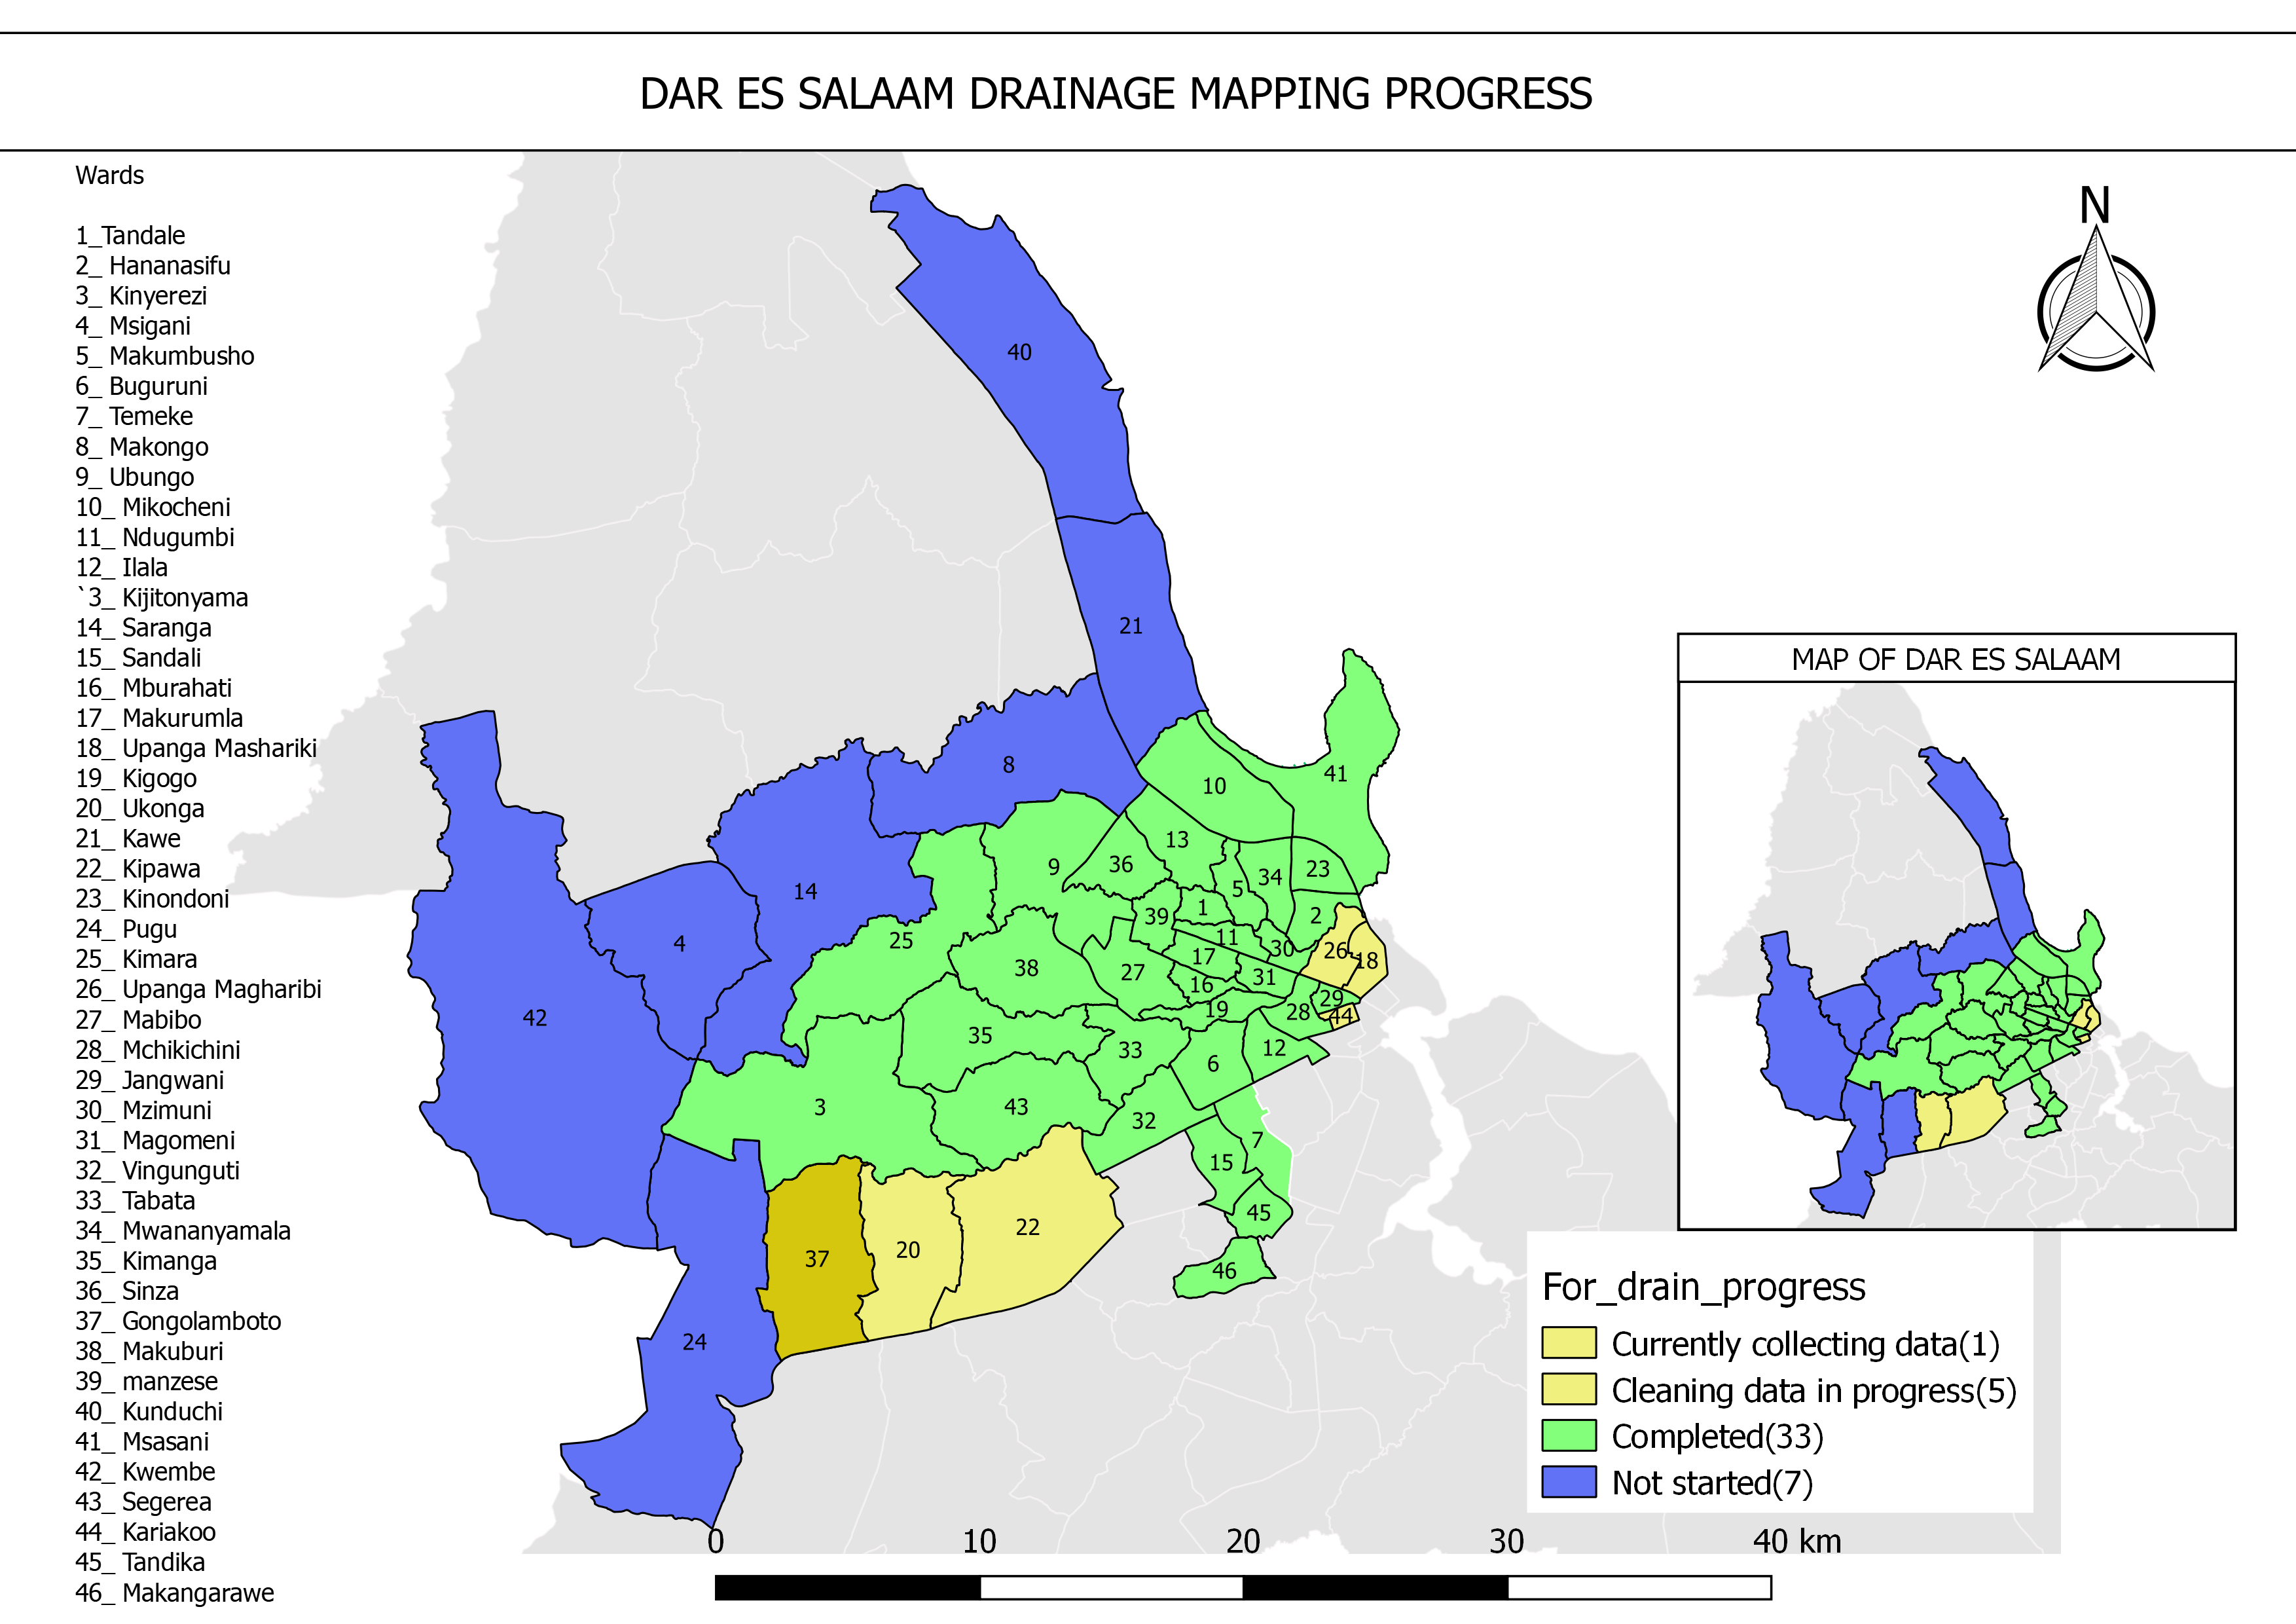
\includegraphics[width=1\textwidth]{images/Dar_drainage_mapping_progress.png}
\end{figure}

\subsubsection{Data Collection Methodology}

{\color{RHblue} Data collection}
\
Preparation of field paper (soft copy) in KoBo Toolbox for the ODK application for drain segments and points. Field mappers then installed ODK on their Android phones and with the URL for the server to be used, they downloaded the survey forms, filled the required information from the field and uploaded the forms.


\subsubsection{Data Model}
\href{https://wiki.openstreetmap.org/wiki/Dar_es_Salaam/Ramani_Huria\#Drainage}{Dar es Salaam\_Ramani Huria\_OpenStreetMap Wiki}\footnote{\url{https://wiki.openstreetmap.org/wiki/Dar_es_Salaam/Ramani_Huria\#Drainage}}

\subsubsection{Timeline}
August, 2017 and Ongoing

\subsubsection{Quality Assurance}
During the data cleaning process, the ODK forms that were filled in the field are downloaded from the server in Comma Separated Value (CSV) format and converted to GeoPackage (.gpkg) in QGIS. The plugin to convert ODK form to CSV format is found in \href{https://github.com/zestyping/odk_csv}{GitHub}\footnote{\url{https://github.com/zestyping/odk\_csv}}. The drain segments and points are styled with a pre-defined .qml style found in QGIS---Drain\_lines\_categorized\_with\_labels\_and\_directions and Drain\_points\_categorized\_with\_labels. After the data is cleaned, it is run in the \href{https://github.com/openearth/hydro-osm}{Hydro OSM model}\footnote{\url{https://github.com/openearth/hydro-osm}} to ensure all drain segments and points are connected.

The team also used QGIS with pre-installed template styles for the segments and points, a high resolution 2016 COWI imagery.

\subsubsection{Access}
\begin{itemize}
    \item \href{https://geonode.uhurulabs.org/layers/geonode\%3ADrain\%20Segments}{UhuruLabs\_Drain Segments}\footnote{\url{https://geonode.uhurulabs.org/layers/geonode\%3ADrain\%20Segments}}
    \item \href{https://geonode.uhurulabs.org/layers/geonode\%3ADrain\%20Points}{UhuruLabs\_Drain Points}\footnote{\url{https://geonode.uhurulabs.org/layers/geonode\%3ADrain\%20Points}}
\end{itemize}

\subsubsection{Licensing}
\href{https://creativecommons.org/licenses/by/4.0/}{CC-BY 4.0}\footnote{\url{https://creativecommons.org/licenses/by/4.0/}}

\subsubsection{Statistics}
38 out of 44 wards of Dar es Salaam Ramani Huria prioritized wards completed. 


Number of segments culverts, drains, ditches and decommissioned (destroyed or burried) mapped are 16207 with 653 kilometers and 12620 number of drain points.
This is summerised in the table below

\begin{center}
\begin{table}[h]
    \centering
    \begin{tabular}{ c|c|c|c }
    \hline
     Number of Segments & 16207 \\
     \hline
     Number of Points & 12620 \\
    \end{tabular}
\end{table}
\end{center}

\subsubsection{Data Visualization}
\begin{figure}[h]
  \centering
  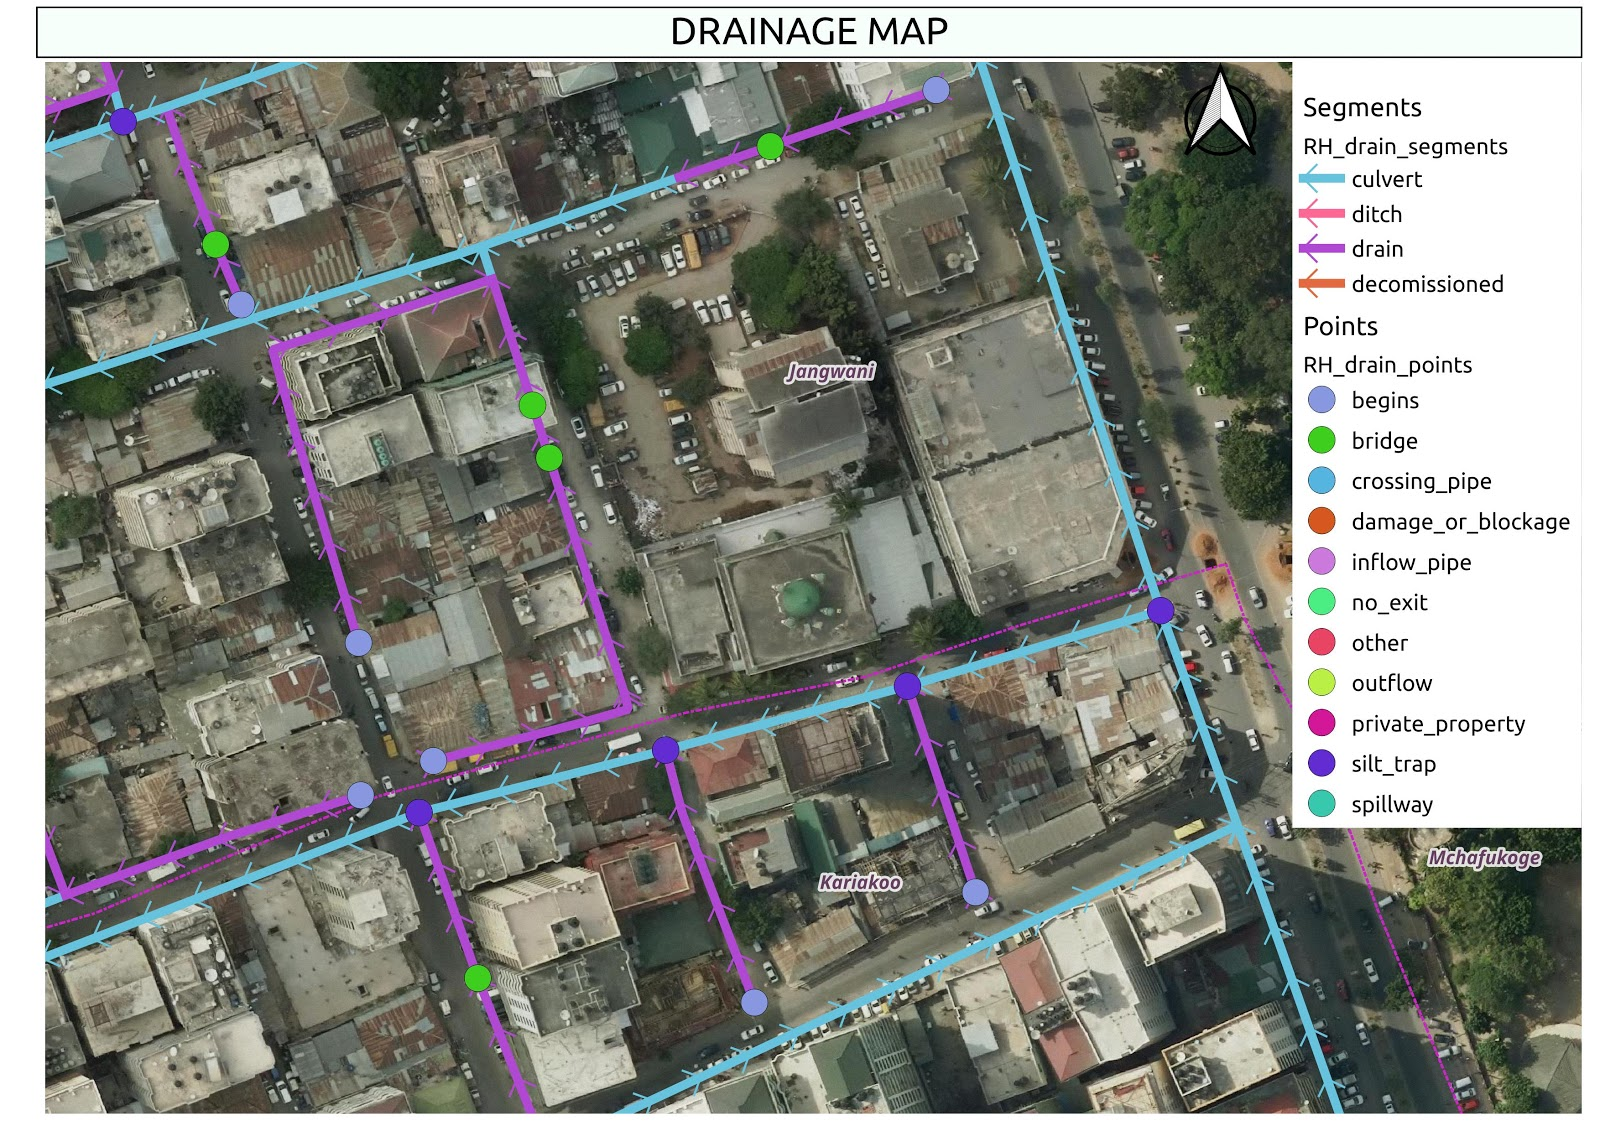
\includegraphics[width=0.8\textwidth]{images/Drainage_Visualization.jpeg}
\end{figure}

\subsubsection{Use Case}
Development of a flood model and early warning systems

\subsubsection{Data Gap}

\subsubsection{Lessons Learned}

\newpage
\subsection{Soil Sediment Sampling}

Soil sediment profiles giving the soil particle sizes for surface and subsurface soils. Contains 643 soil sample points in a 2km by 2km grid covering Dar es Salaam.
Useful for erosion modeling, also potentially agriculture and building planning. 

\subsubsection{Spatial Extent}
Dar es Salaam and neighboring districts of Pwani region i.e. Bagamoyo, Kibaha and Kisarawe.

\begin{figure}[h]
  {\color{RHblue}\caption{A geo-referenced set of soil sediment profiles in Dar es Salaam and Pwani regions}}
  \centering
  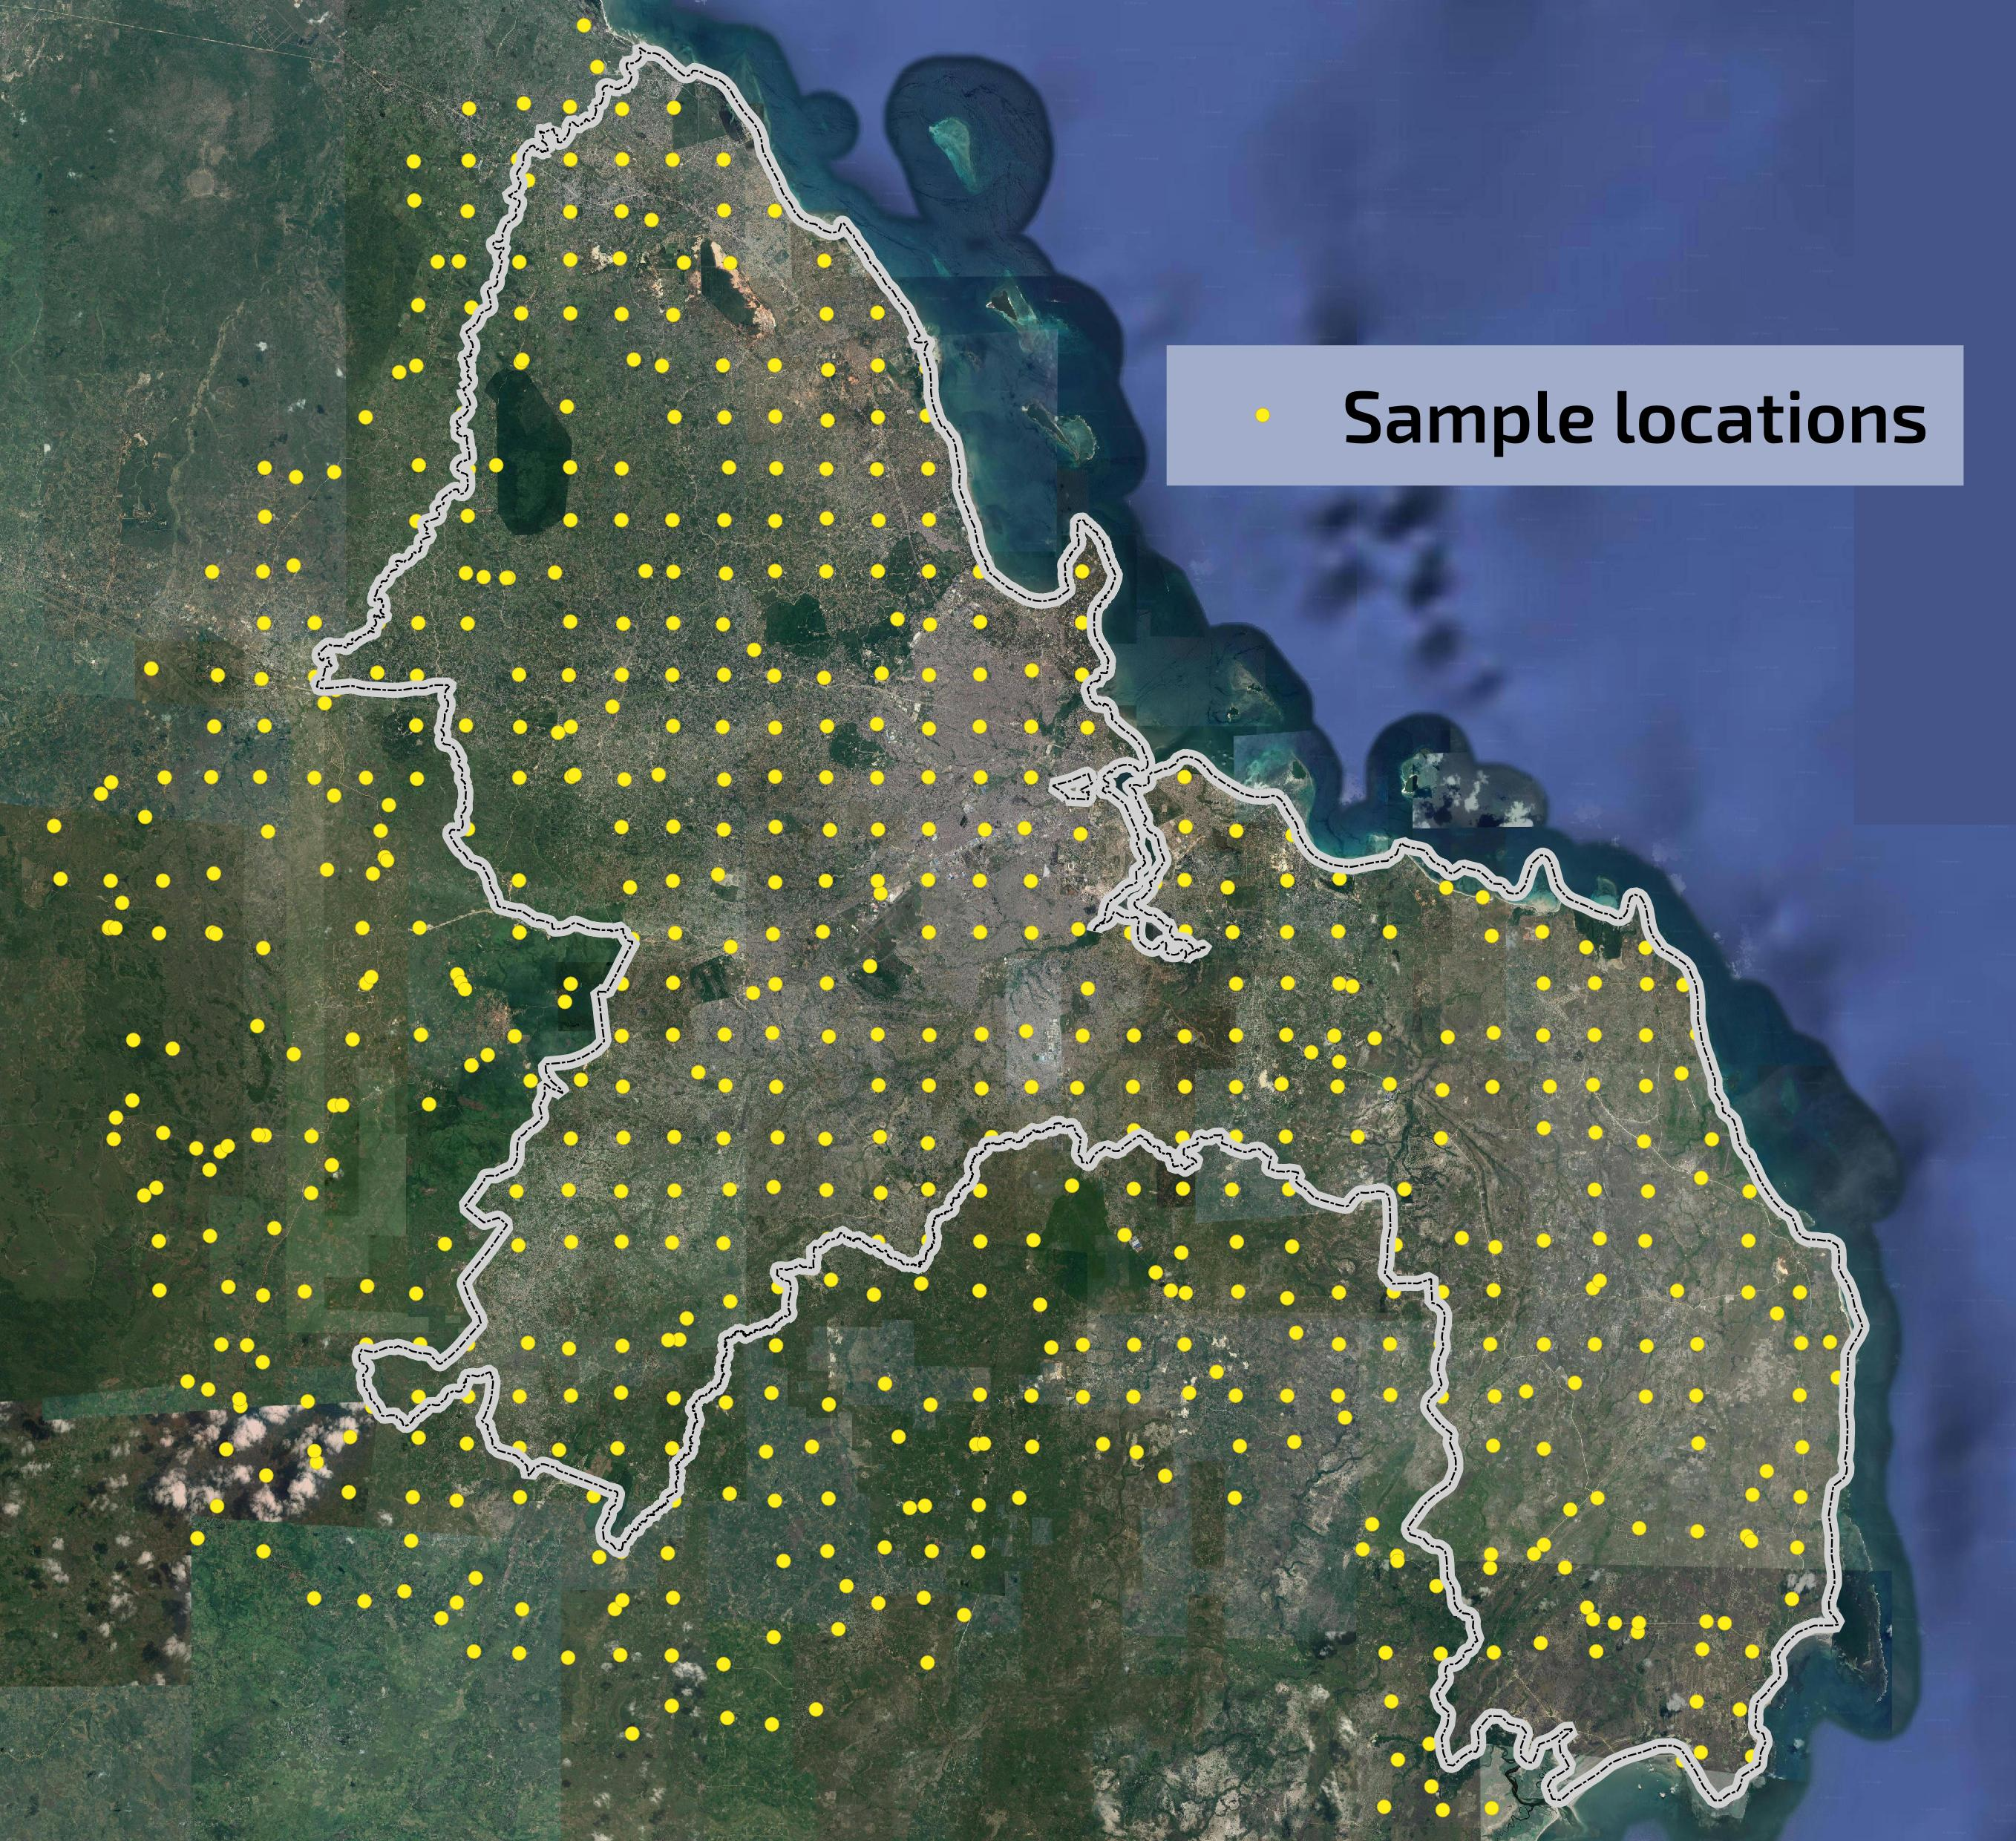
\includegraphics[width=0.8\textwidth]{images/soil_sample_locations.jpg}
\end{figure}

\subsubsection{Data Collection Methodology}

\begin{multicols}{2}
We created 2km by 2 km grid points. A set of data was recorded at each site using OpenDataKit’s Android application ODK Collect. Each field sampling team of two people carried the following equipment: trowel or small shovel, plastic “ziploc” bags with 1kg capacity, Android phone pre-loaded with ODK Collect---a separate maps and navigation application, maps.me---pre-loaded with the locations to be visited, first aid kit, marker pens, permission letter for the sampling activity from the municipal authorities and a tape measure.

We got training from a geo-morphologist and set up our own citizen-style lab to analyze the soil samples. The pair of samples—top and bottom—from each site was passed through a set of progressively finer-mesh sieves, resulting in nine separate fractions. Each fraction was weighed. The resulting measurements, which represent the proportion of each sediment particle size at each site, were
recorded.

The following materials were used: a set of metal sieves, scales, hand wash station and gloves, brush, cloth and towel for cleaning sieves, an Android phone with ODK Collect and sieving survey.
\end{multicols}

\subsubsection{Data Model}

\subsubsection{Timeline}
2018-10-11 to 2019-02-23

\subsubsection{Quality Assurance}

The quality control was done by  using ODK form to flag out any discrepancies such as negative masses or discrepancies in sums immediately.

\subsubsection{Access}
\href{https://geonode.uhurulabs.org/layers/geonode\%3A_2019_02_26_dar_soil_sampling_final_results_v1}{UhuruLabs\_Soil Sediment Sampling}\footnote{\url{https://geonode.uhurulabs.org/layers/geonode\%3A20190226darsoilsamplingfinalresultsv1}}

\subsubsection{Licensing}
CC-BY 4.0

\subsubsection{Statistics}
731 soil sample points created using a 2 km grid. 643 points sampled and sieved; 88 sample points were either inaccessible or hard to collect sample e.g. paved areas, military base.

\subsubsection{Data Visualization}
\begin{figure}[h]
  \caption{A detail of the map showing the soil particle size in Dar es Salaam. The upward-facing histogram bars represent the top (surface) samples, and the downward-facing bars represent the bottom samples.}
  \centering
  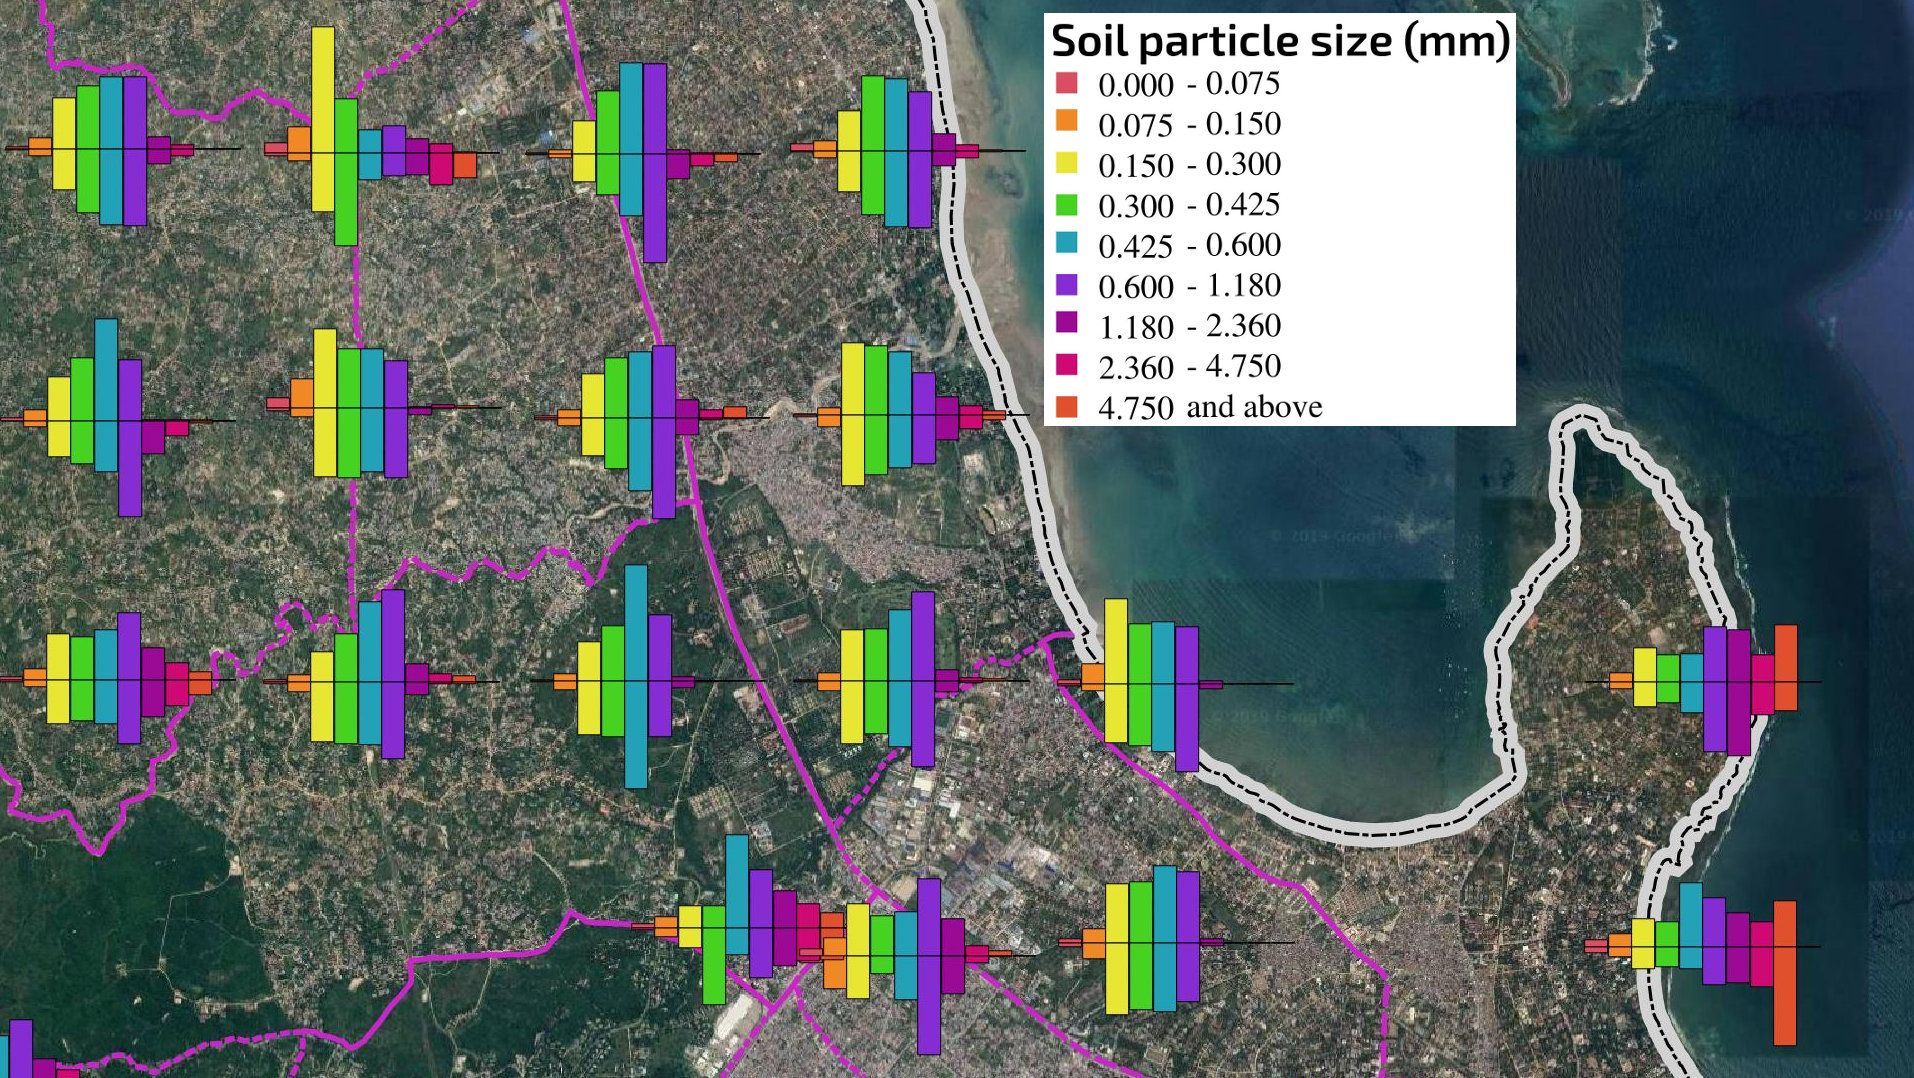
\includegraphics[width=1\textwidth]{soil_map_detail_peninsula_with_legend}
\end{figure}

\subsubsection{Use Case}
JBA  primarily intended for use this data for erosion modeling. The resulting dataset, a geo-referenced set of soil profiles, has been published as open data.

\subsubsection{Data Gap}
We have size of particles and maps but there is no data showing the chemical decomposition of soil.

\subsubsection{Lesson Learned}
{\color {RHblue}Budgeting time for seeking permissions-}
\
A common challenge in this type of activity is seeking permission for doing what may be suspicious-looking activities (running around random areas of a major city with a shovel, for example).

{\color {RHblue}Inconsistent offset procedure-}
\
Looking at the map of the sites that were actually collected, there were several for which it is not precisely clear what offset procedure was actually used when a given grid site was not accessible.

{\color{RHblue}Failure to realize the sensitivity of the error thresholds-}
\
When looking at individual measurements anecdotally, we found that most were of high quality. In other words, it was possible to examine a few dozen measurements and only find one or two potential errors, which on the surface appeared to show that things were going well. This was grossly misleading!

{\color{RHblue} Field work outpacing analysis, insufficient early feedback-}
\
As the team felt that the field work would be the most difficult part (and certainly it was the larger consumer of time and resources), we focused on it, and failed to become alarmed when the analysis (sieving) work fell behind. This contributed to there being a substantial backlog of sieving to be done at the end of the field collection, but also contributed to our not discovering the high proportion of discrepancies until long after the field work was complete.

{\color{RHblue}Inadequate backup of samples-}
\
We did not build backup into our analysis; we discarded all of the sediment immediately after sieving and measurement, and only collected enough for a single round of sieving at each site.

{\color{RHblue}Data entry system design-}
\
It’s critical to design the tools carefully. We encountered problems in data entry, in part because we didn’t invest enough in making sure the system was robust and simple.

Management of data is highly needed to avoid unnecessary cost.

\newpage

\subsection{Community Assets and Threats}

\begin{multicols}{2}
Flood risk identification on flood prone areas of the city by conducting a series of meetings with key people on specific subwards. Use of influential community members and leaders to identify assets (things that are important to the community), threats (things that the community "thinks" may flood if the hazard continues unabated) and issues that contribute to flooding in their subwards. This information can only be provided by the community itself since they understand their neighbourhoods better.
\end{multicols}

\subsubsection{Spatial Extent}
The inventory covered  243 subwards in 49 wards of Dar es Salaam. 
\begin{figure}[h]
  \color{RHgreen}\caption{49 Wards covered during the community asset and threat mapping inventory}
  \centering
  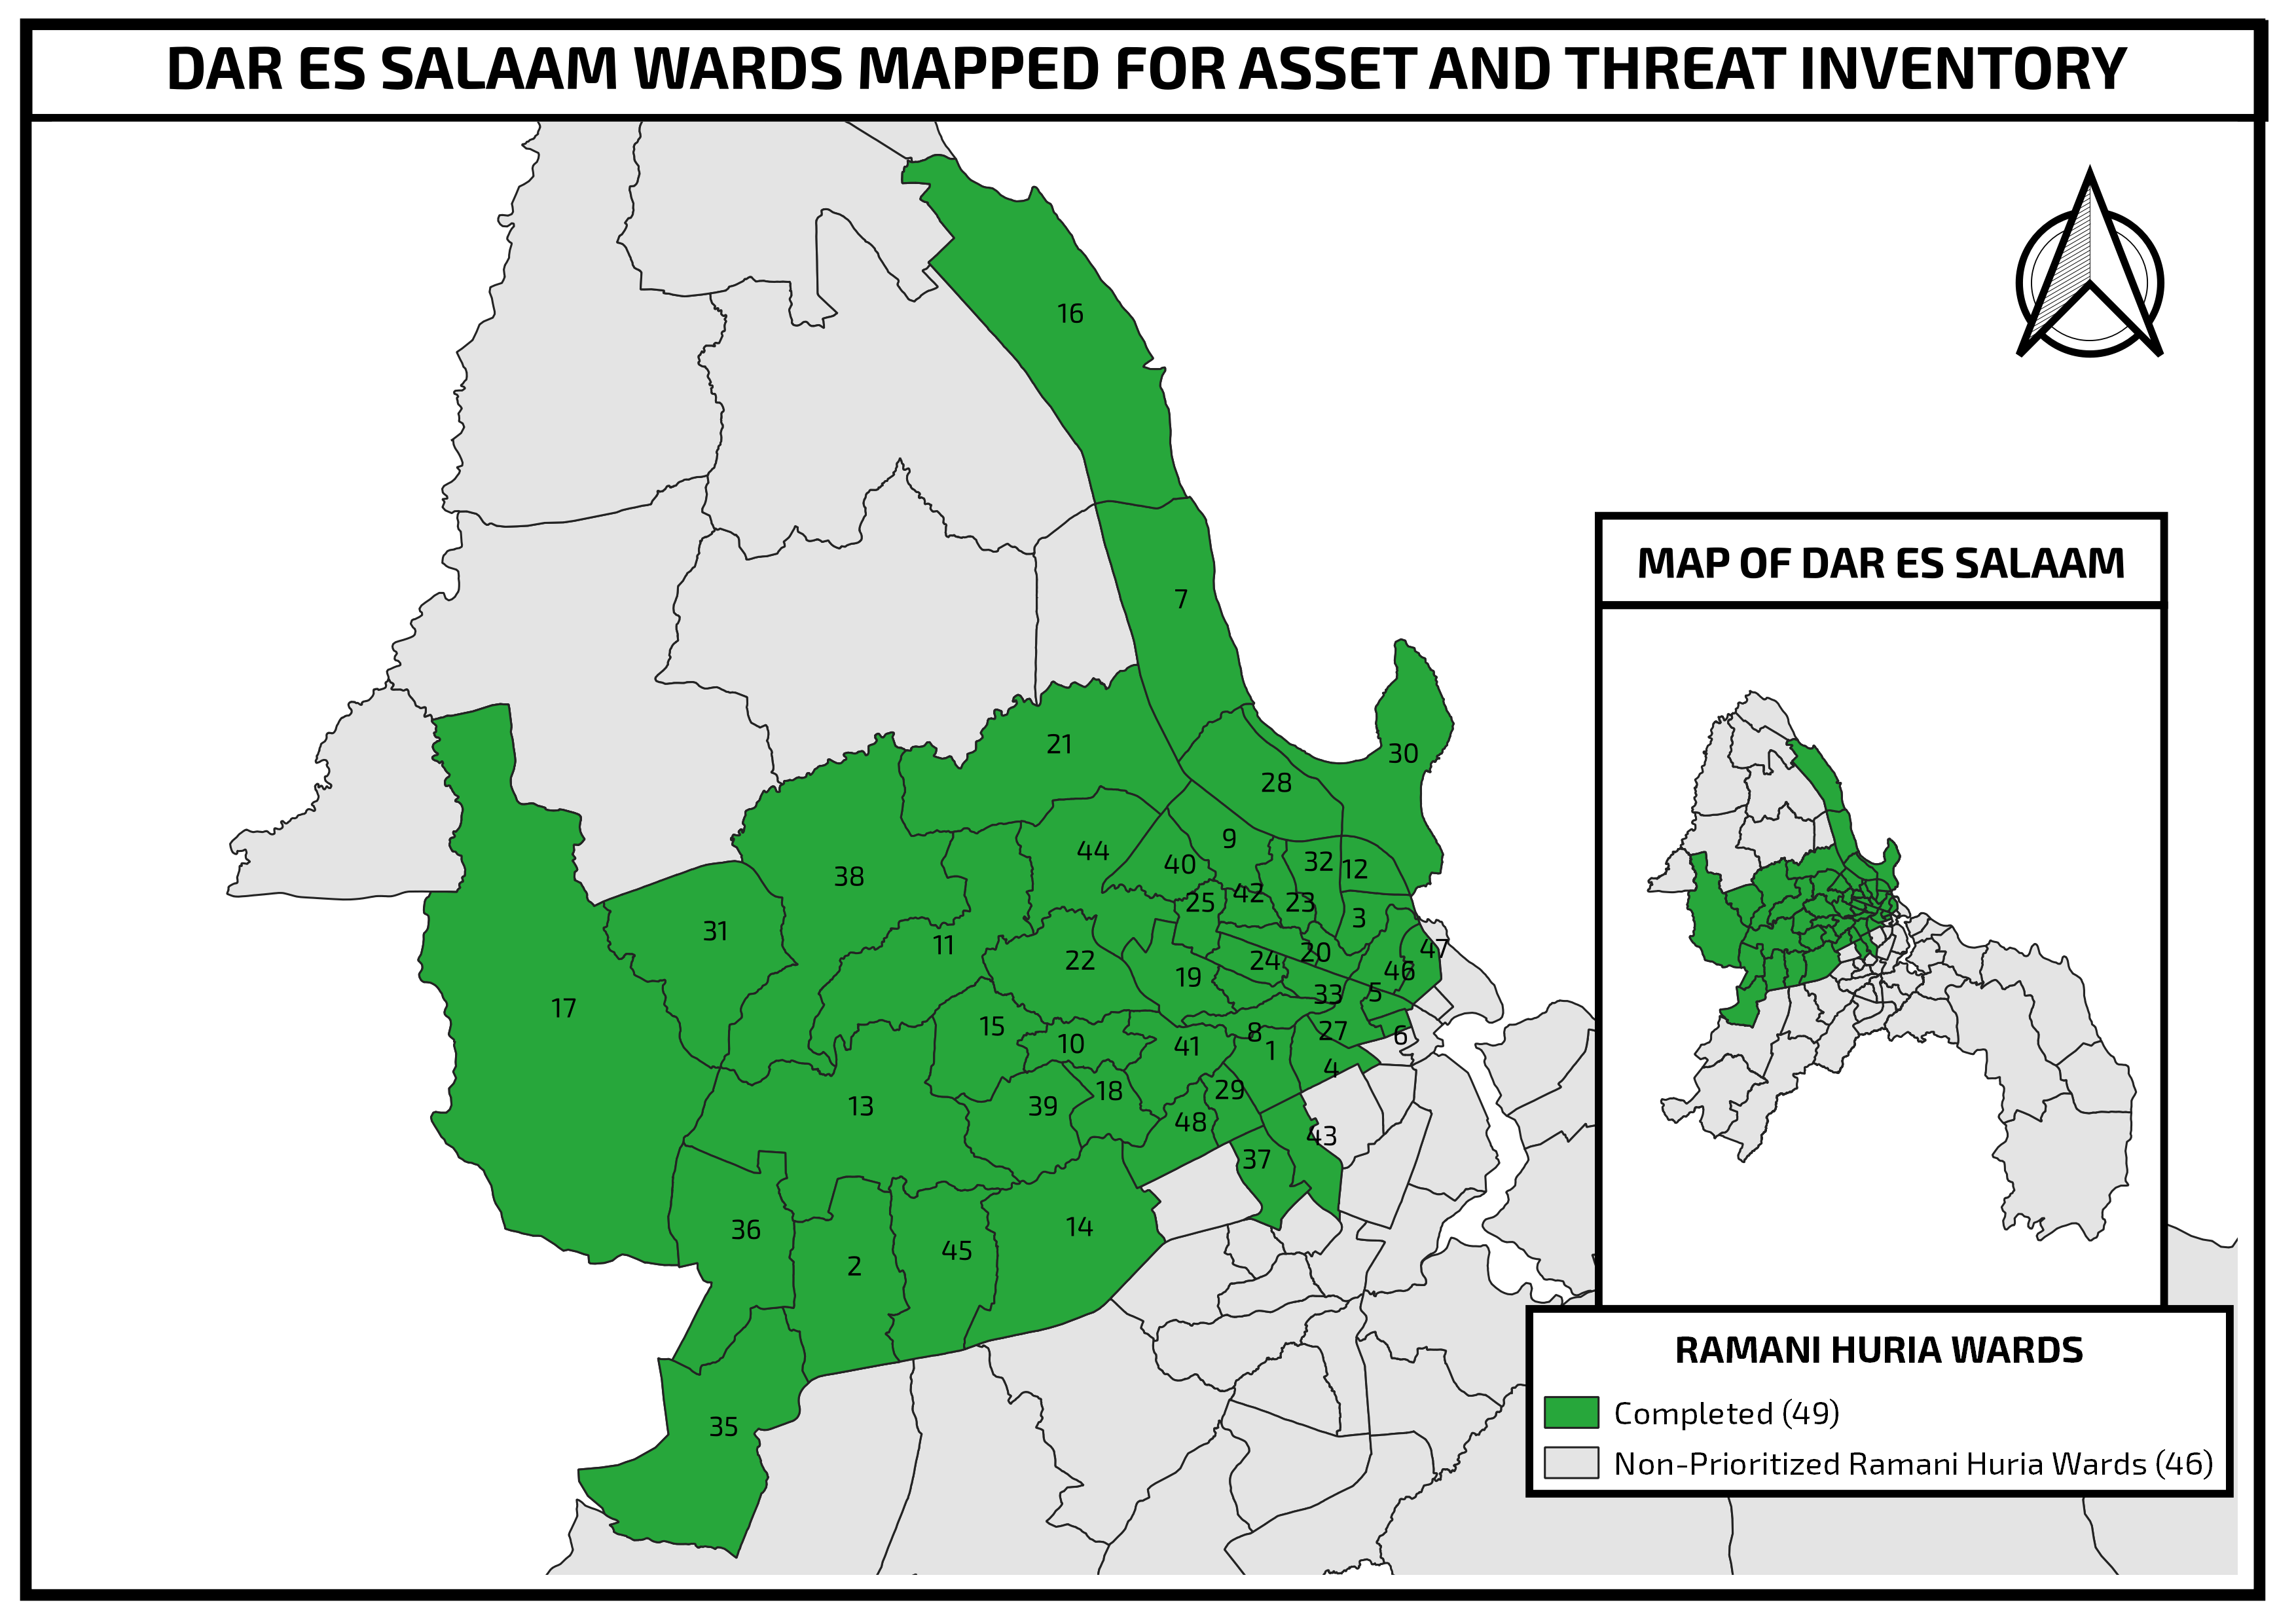
\includegraphics[width=0.8\textwidth]{images/Asset&Threat.png}
\end{figure}
\subsubsection{Data Collection Methodology}
\begin{multicols}{2}
Setting up meetings with community leaders and influential people i.e. religious leaders in the specific wards. We first introduced how the data can help in reducing flooding, then ask them to identify and trace their boundaries on a map printed in A1 and point out assets and disaster threats in their neighbourhoods. We also printed satellite image maps of the respective subward to simplify identification of areas in their subwards.

Students worked in groups of six, visiting one subward at a time. After introductions were completed at the ward level, each subward mapping and data collection took approximately  4-5 days to complete. Threat and Asset inventory mappings were conducted in two different ways depending on whether the subward in question was mapped or unmapped. Student mappers split community members into three groups, each group guided by two students.
\end{multicols}


The discussion was based on three major key points:
\begin{enumerate}
    \item Assets (Important things in the subward)
    \item Assets under threats (in case the subward floods)
    \item Main causes of flood in the subward
\end{enumerate}

\subsubsection{Data Model}

\subsubsection{Timeline}
2018-06-08 to 2019-01-20

\subsubsection{Quality Assurance}
JOSM for editing buildings and roads and QGIS for field data analysis. Other sites are used for Quality Assurance for JOSM data are:
\begin{itemize}
    \item \href{https://qa.poole.ch/\#}{QA}\footnote{\url{https://qa.poole.ch/\#}}
    \item \href{http://osmose.openstreetmap.fr}{Osmose}\footnote{\url{http://osmose.openstreetmap.fr}}
    \item \href{http://keepright.at/}{KeepRight}\footnote{\url{http://keepright.at/}}
\end{itemize}

\subsubsection{Access}
\href{https://drive.google.com/drive/u/1/folders/1nW7luOI0A92GKi1vJtUJwt9P88OAzQ6h}{Dar es Salaam Asset and Threat Inventory}\footnote{\url{https://drive.google.com/drive/u/1/folders/1nW7luOI0A92GKi1vJtUJwt9P88OAzQ6h}}

\subsubsection{Licensing}
CC-BY 4.0

\subsubsection{Statistics}
A total of 5020 asset points were collected during the project. These include:
\begin{center}
\begin{tabular}{ |c|c|c| }
 \hline
 Assets at risk but not important & 28 \\ 
 \hline
 Evacuation centers & 42 \\ 
 \hline
 Important assets and at risk & 857 \\
 \hline
 Important assets but not at risk & 4093 \\
 \hline
 Roads and road names & 65868 \\
 \hline
 Landmarks & 1538 \\
 \hline
\end{tabular}
\end{center}

\subsubsection{Data Visualization}

\subsubsection{Use Case}
March, 2019 community flood response, creating resilience plans, mitigation measures through community mapping and impact assessment.

\subsubsection{Data Gap}
Out of 49 wards, historical flood extent was conducted in only 11 wards. There is a need of conducting flood extent in the remaining wards to create a better understanding of flooding.

\subsubsection{Lessons Learned}
Planning on paper vs actual fieldwork. We underestimated the time allocation in the work plan and number of training days which in turn resulted to a crappy work (maps and reports) leading to an  extension of time from October 2018 as the planned completion month to January 2019.

\medskip
We selected a few competent and committed students to re-do the maps and reports.


\newpage
\subsection{Buildings Footprint Digitization}
\begin{multicols}{2}
Re-digitization of the city to update and improve the quality of already digitized layers using COWI imagery with 10cm resolution provided by the Ministry of Lands, Housing and Human Settlements. (Previously the city was digitized using either Bing, Mapbox or Digitalglobe which have lower resolutions compared to COWI imagery. So far the team has been able to digitize 28 out of 44 Ramani Huria wards. Namely Kisutu, Temeke, Vingunguti, Upanga Mashariki, Upanga Magharibi, Jangwani, Sandali, Kivukoni, Mwananyamala, Tabata, Kigogo, Kariakoo, Gerezani, Mchikichini, Hananasifu, Sinza, Kjitonyama, Magomeni, Tandale, Buguruni, Ilala, Keko, Mbagala, Mbagala kuu, Mabibo, Mchafukoge and Mzimuni. The wards digitized have a total of 299,691 buildings. This number includes new and existing buildings altogether.
\end{multicols}

\subsubsection{Spatial Extent}
28 out of 44 Ramani Huria prioritized wards in Dar es Salaam have been re-digitized
\begin{figure}[h]
  \caption{28 prioritized Ramani Huria wards have been re-digitized by the team}
  \centering
  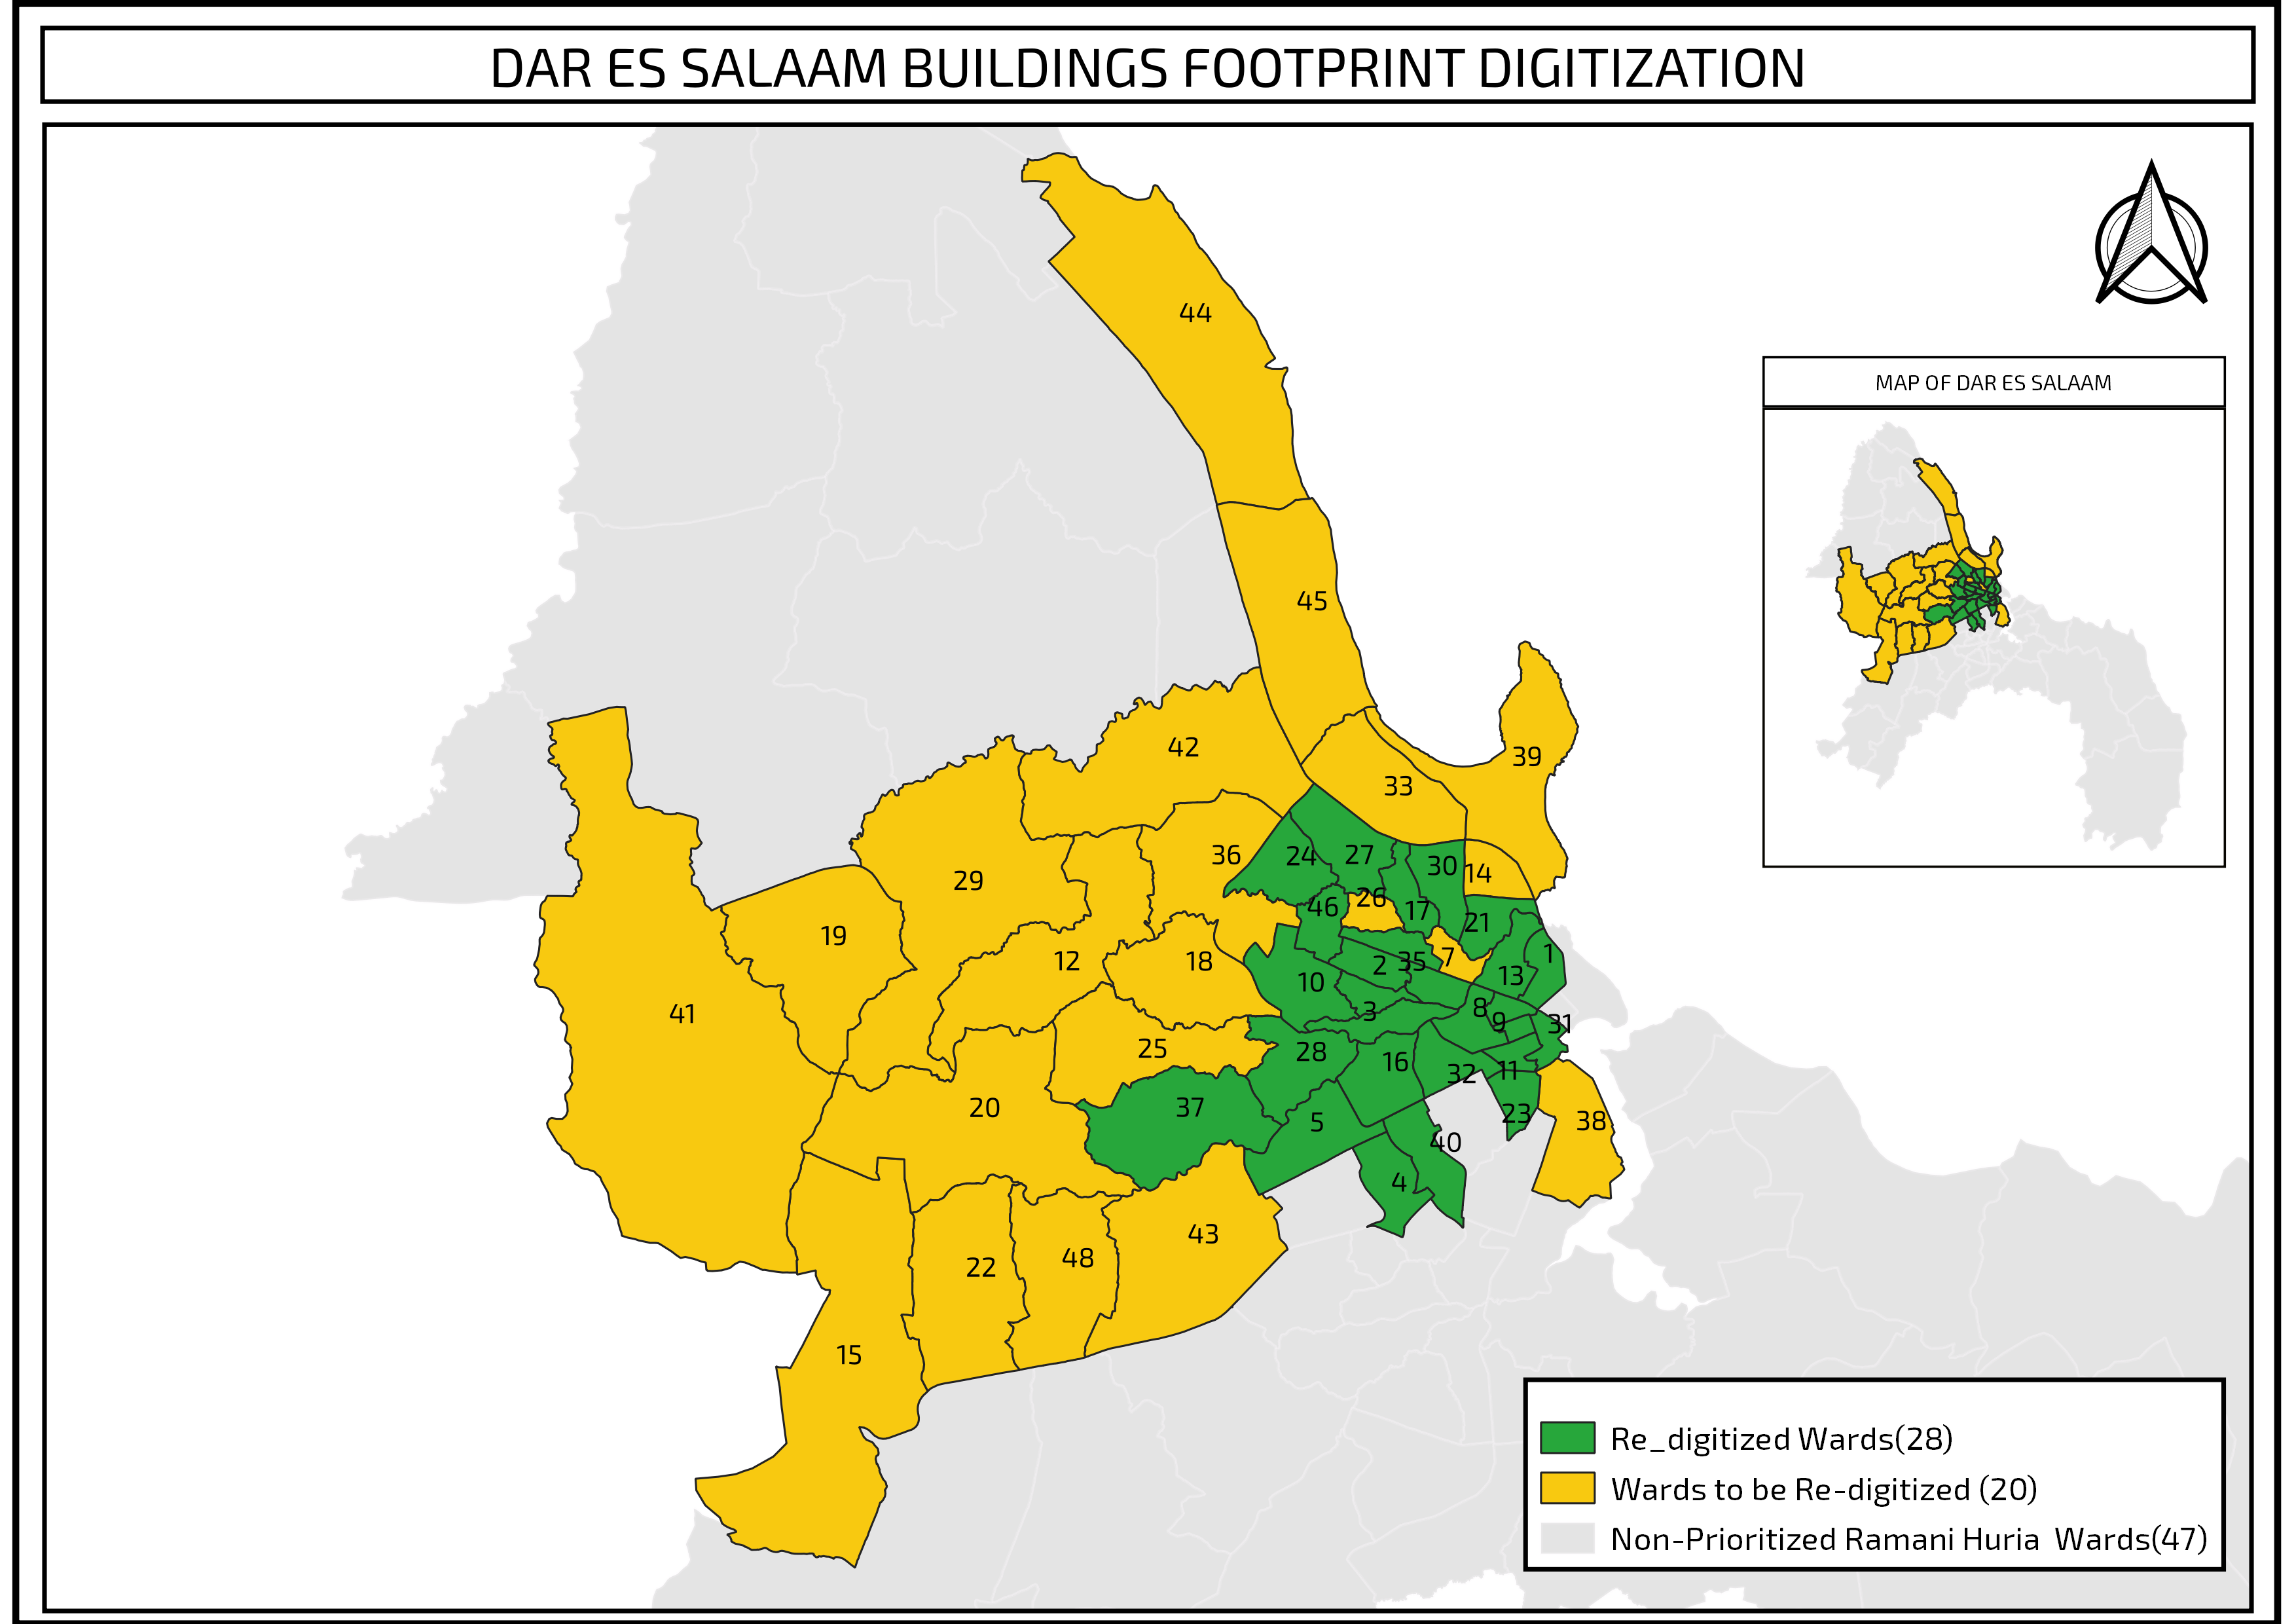
\includegraphics[width=1\textwidth]{images/Building_Footprint_Digitization.png}
\end{figure}


\subsubsection{Data Collection Methodology}

The purpose of the work was introduced to the team and mbtiles for the wards were created in \href{https://www.gdal.org/gdaladdo.html}{GDAL}\footnote{\url{https://www.gdal.org/gdaladdo.html}} (gdaladdo)---a utility used to build or rebuild overview images. Supervisors of the team created mapping projects on \href{https://tasks.hotosm.org/}{HOT Tasking Manager}\footnote{\url{https://tasks.hotosm.org/}} which were then assigned to the digitization team. Using the 2016 COWI imagery, buildings were re-digitized in JOSM and validation of the re-digitization was done by the validation team.

\subsubsection{Data Model}
\href{https://wiki.openstreetmap.org/wiki/Dar_es_Salaam/Ramani_Huria\#Buildings}{Dar es Salaam\_Ramani Huria\_OpenStreetMap Wiki}\footnote{\url{https://wiki.openstreetmap.org/wiki/Dar_es_Salaam/Ramani_Huria\#Buildings}}

\subsubsection{Timeline}
2018-08-24 to 2018-10-20

\subsubsection{Quality Assurance}
\begin{itemize}
    \item JOSM
    \item Tasking Manager
\end{itemize}

\subsubsection{Access}
\href{https://drive.google.com/drive/u/1/folders/1Aly4pDcq5JP14vB6VY-IxahTwvt6Ukrv}{Dar es Salaam Buildings}\footnote{\url{https://drive.google.com/drive/u/1/folders/1Aly4pDcq5JP14vB6VY-IxahTwvt6Ukrv}}

\subsubsection{Licensing}
\href{https://opendatacommons.org/licenses/odbl/index.html}{Open Data Commons Open Database License (ODbL)}\footnote{\url{https://opendatacommons.org/licenses/odbl/index.html}}

\subsubsection{Statistics}
\begin{center}
\begin{tabular}{|c|c|}
\hline
   Buildings before re-digitization & 460,917 \\
\hline
   Buildings after re-digitization & 677,478 \\
\hline
\end{tabular}
\end{center}

\subsubsection{Data Visualization}
\begin{figure}
  \begin{subfigure}[b]{0.5\textwidth}
    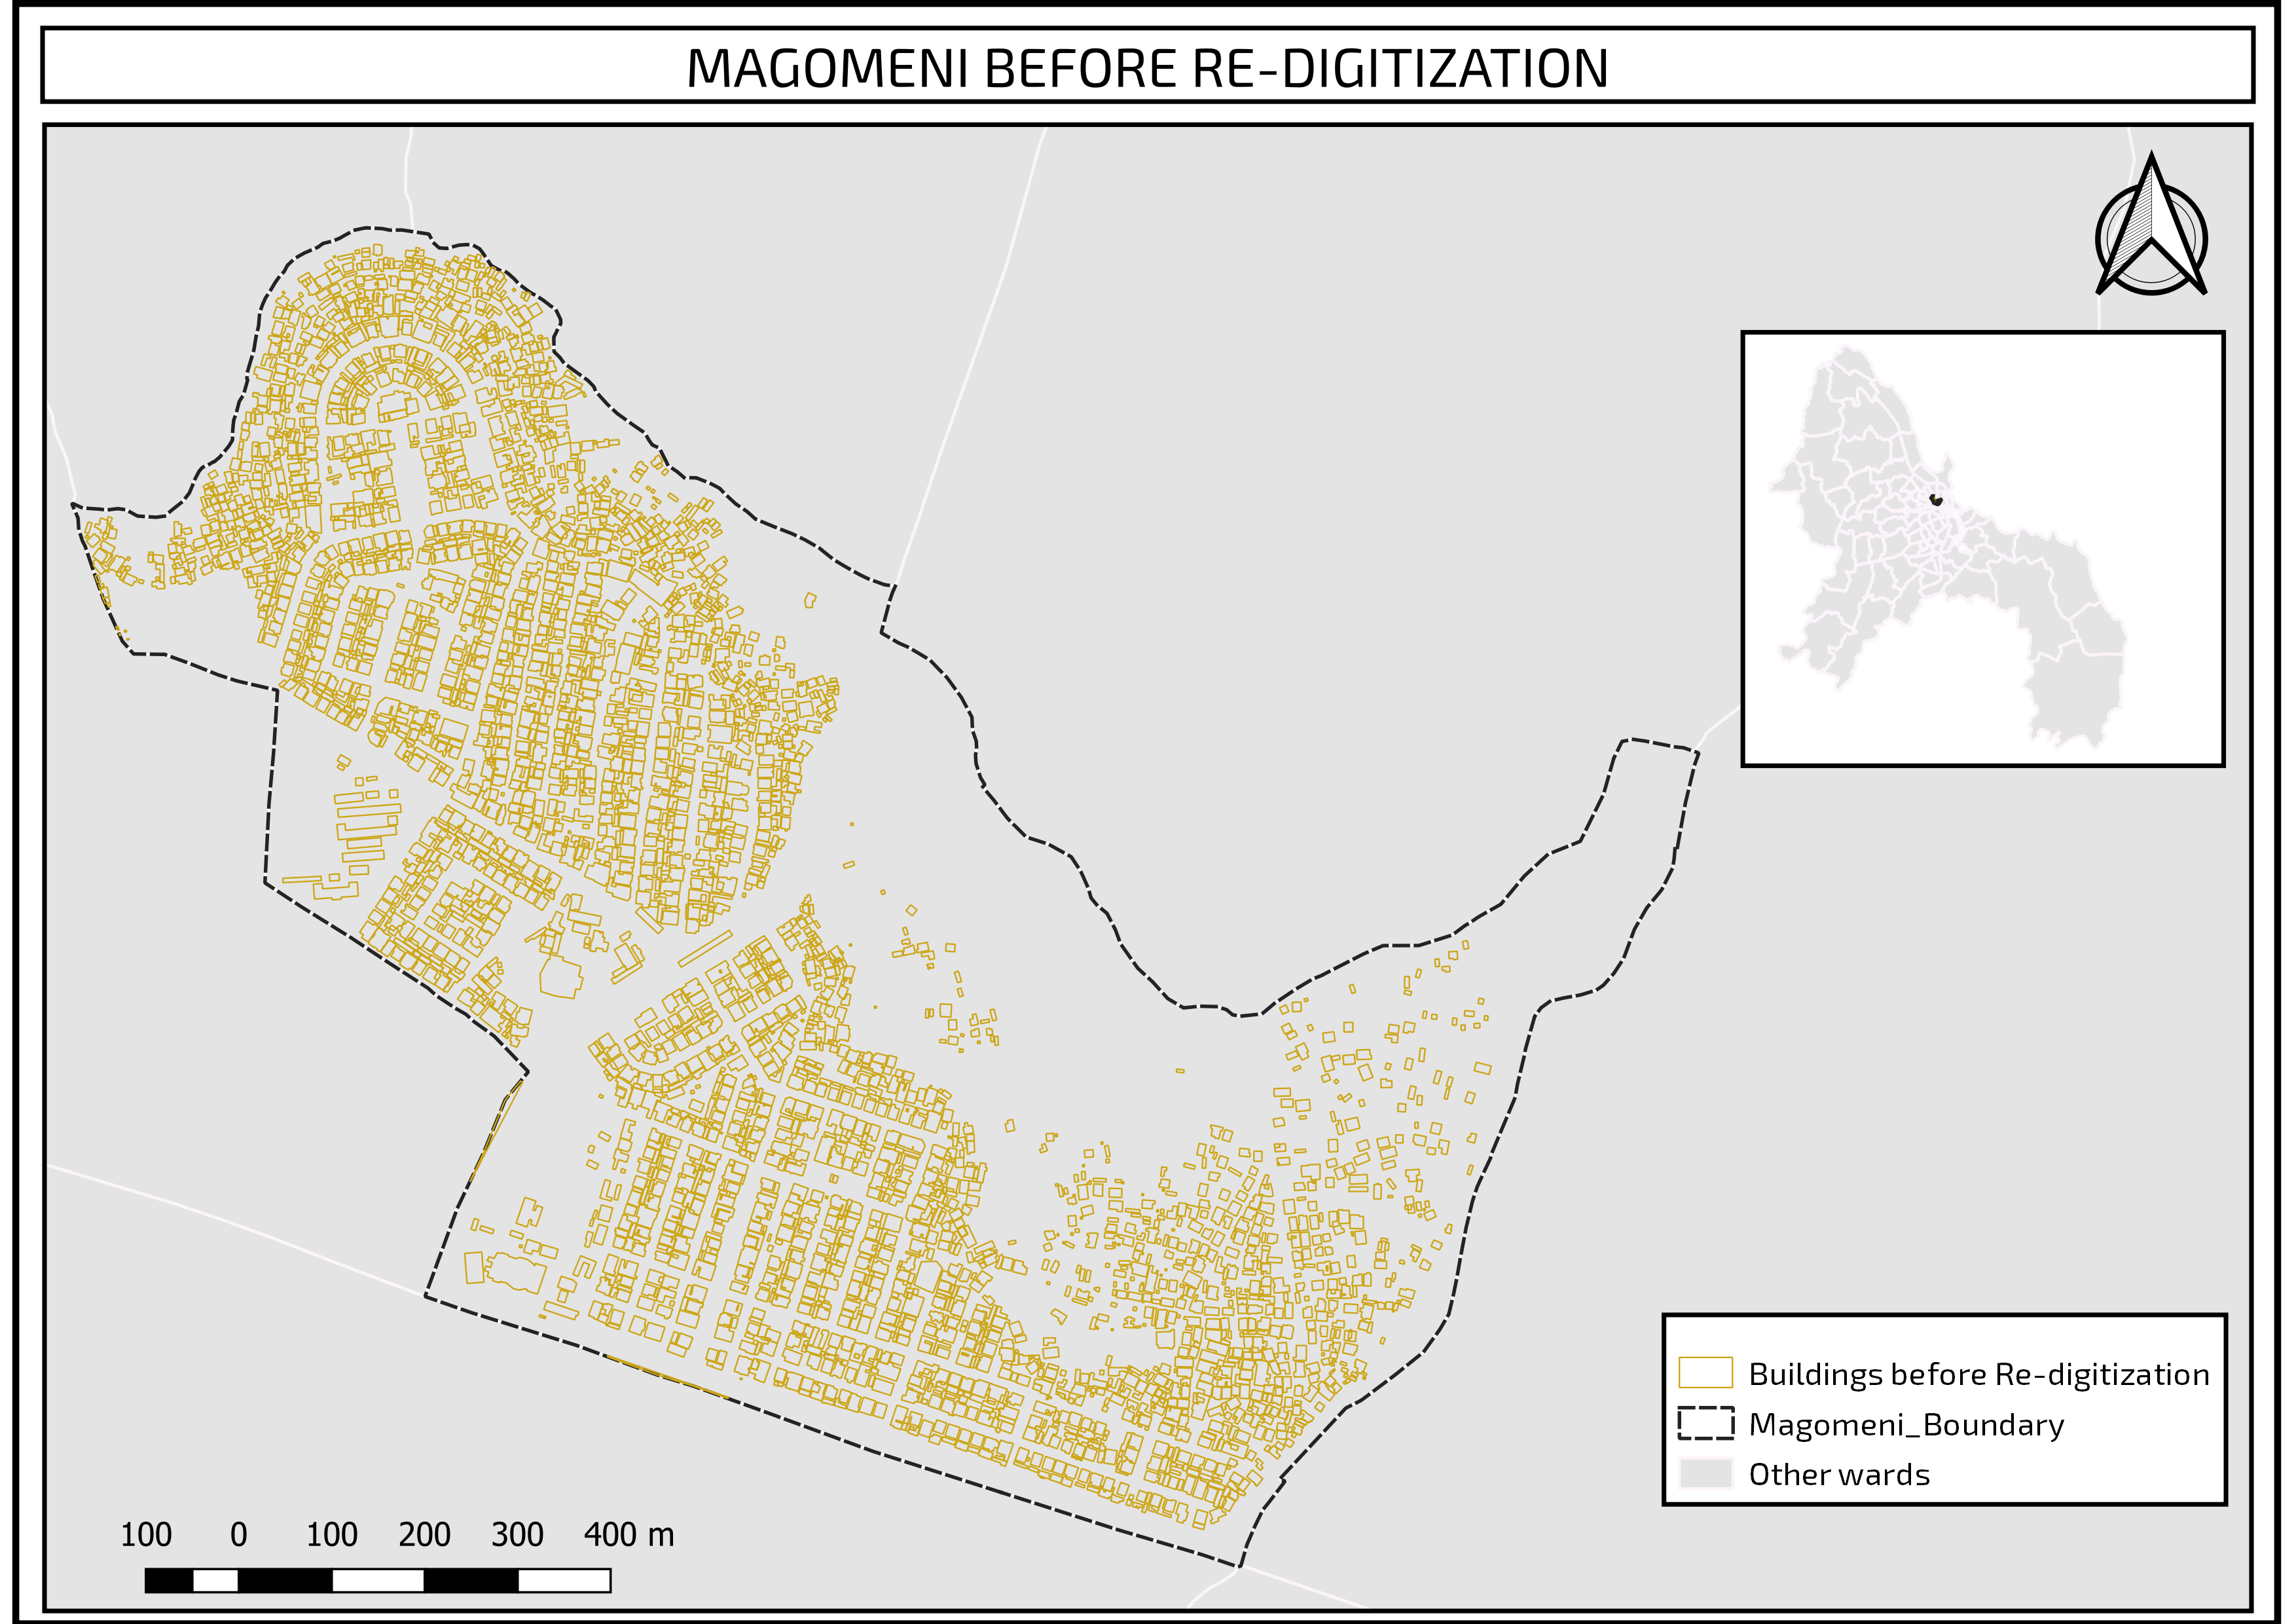
\includegraphics[width=\textwidth]{Magomeni_Before_Redigitization.png}
   \color{RHgreen}\caption{Map showing Magomeni ward before re-digitization using UAV imagery}
    \label{fig:1}
  \end{subfigure}
  %
  \begin{subfigure}[b]{0.5\textwidth}
    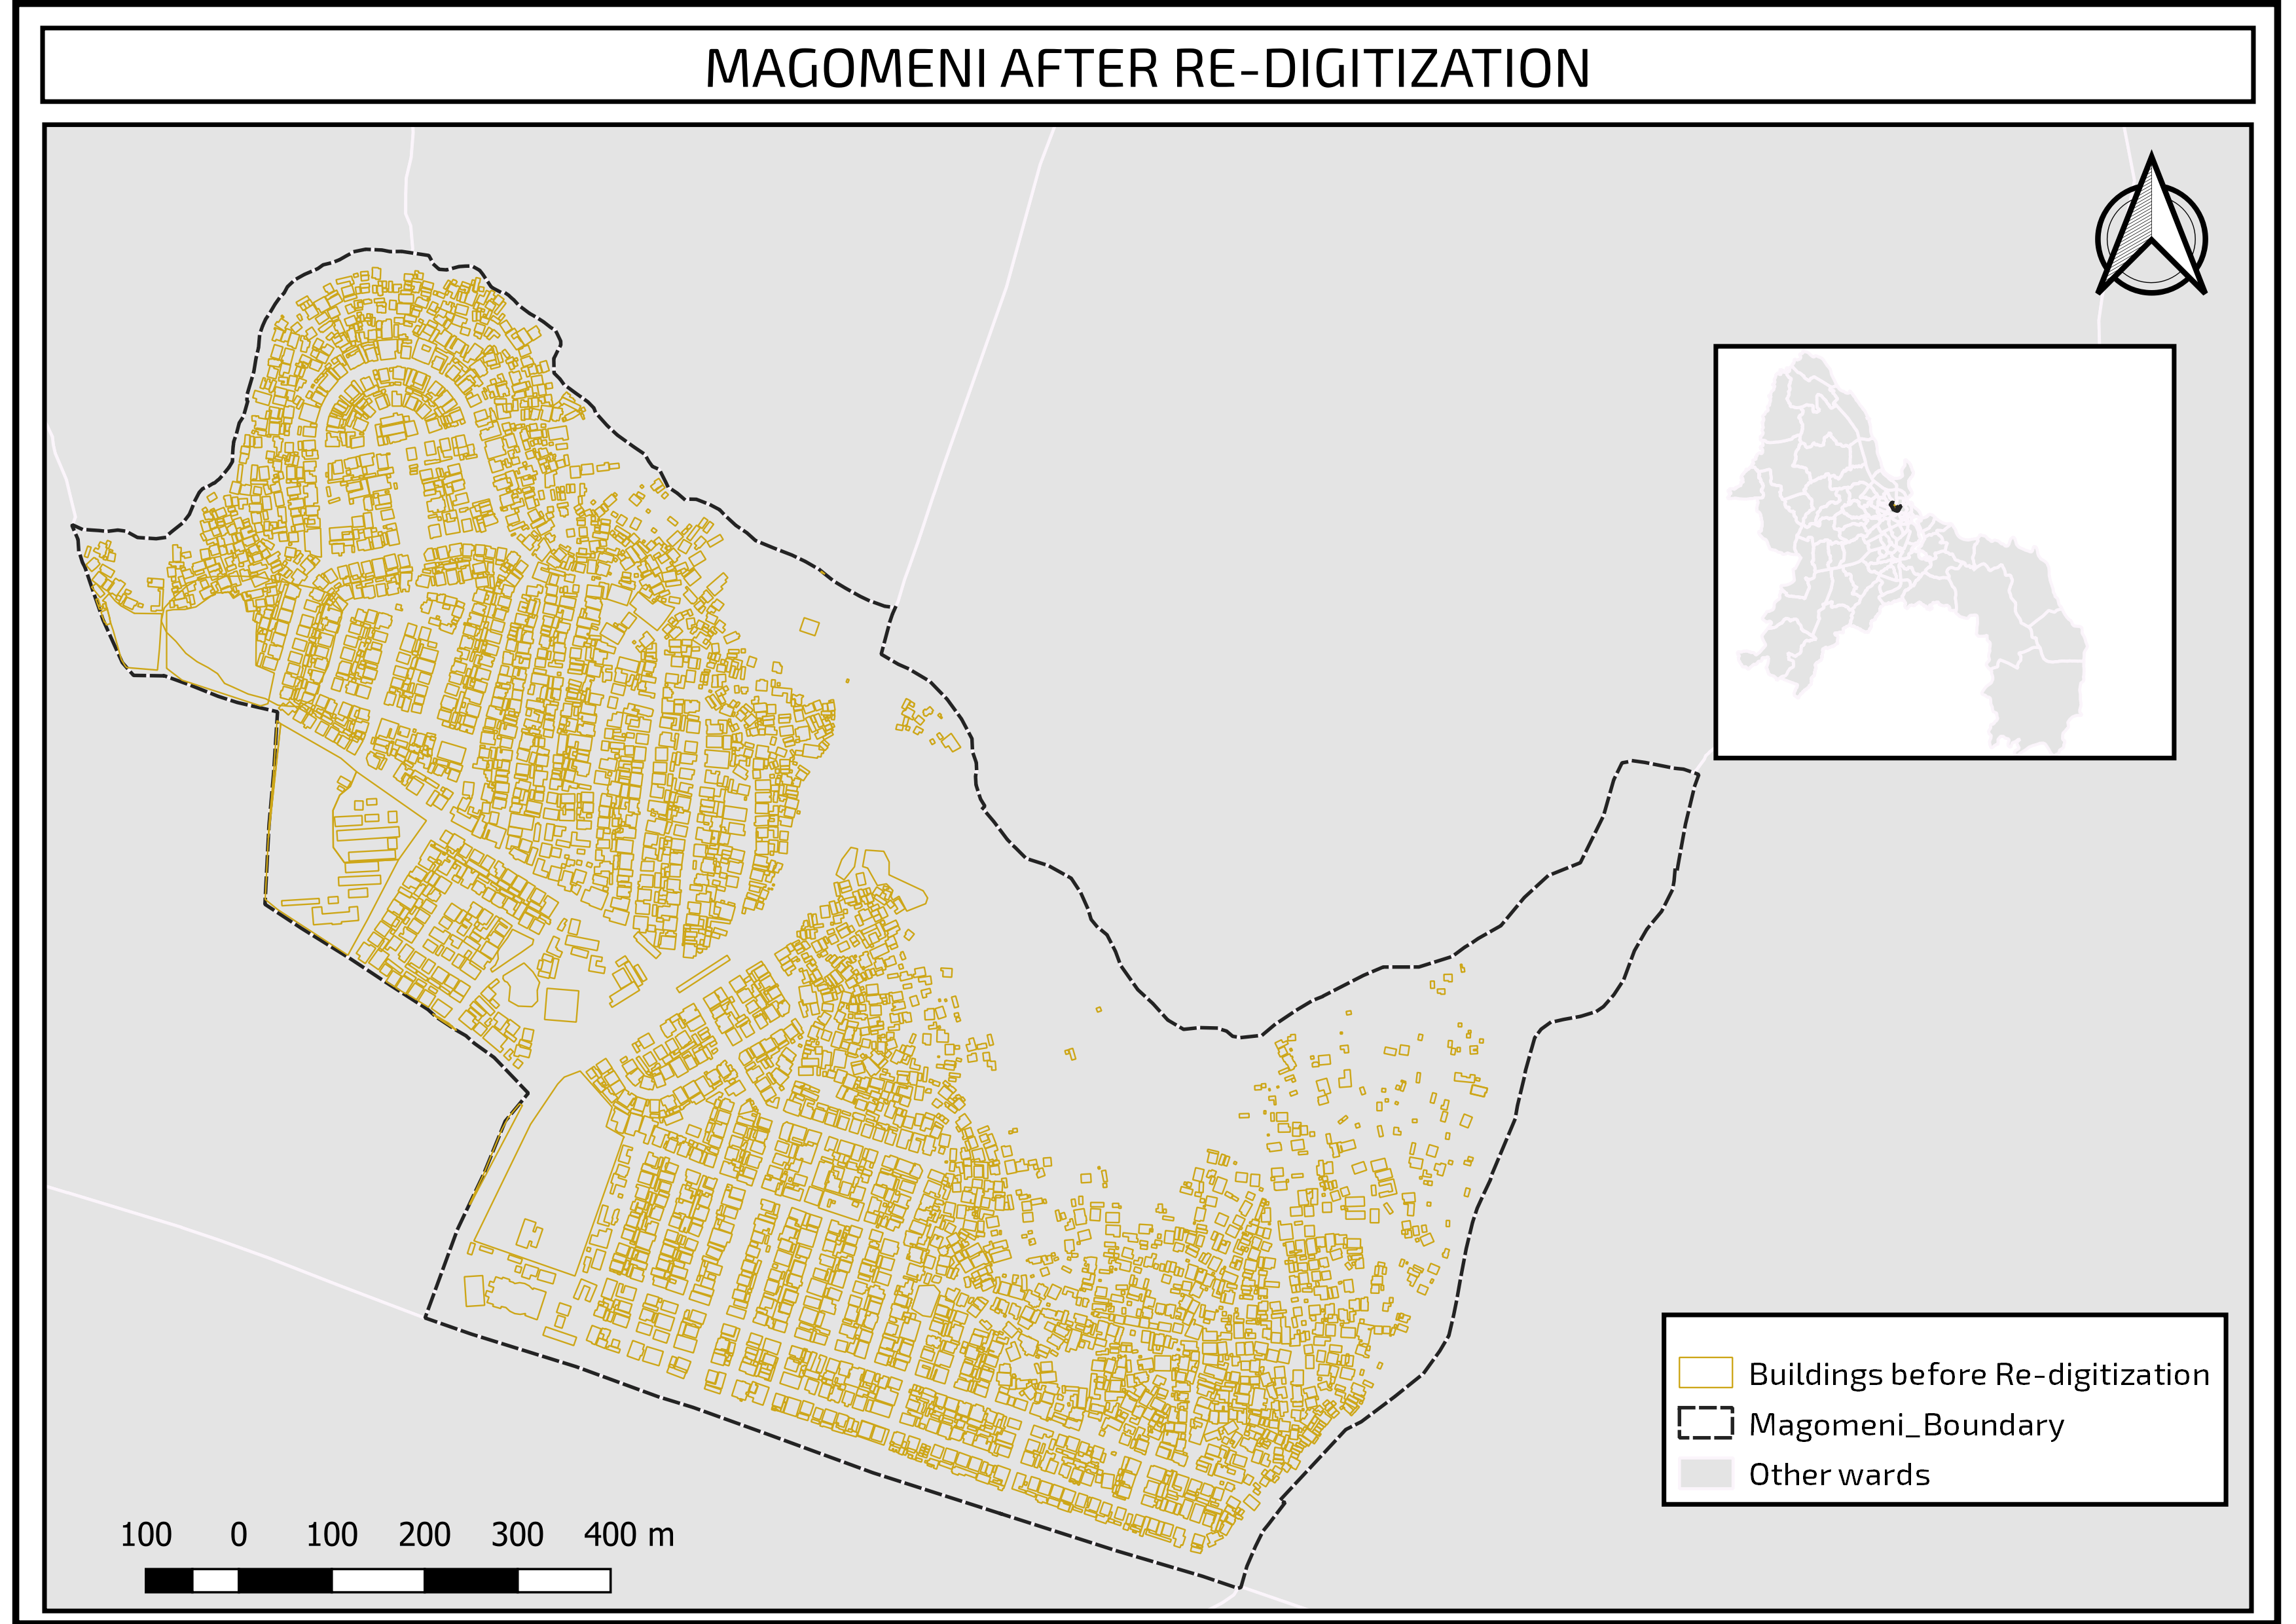
\includegraphics[width=\textwidth]{Magomeni_After_Redigitization.png}
    \color{RHgreen}\caption{Map showing Magomeni ward after re-digitization using UAV imagery}
    \label{fig:2}
  \end{subfigure}
\end{figure}

 \vspace{2mm}
 
\begin{figure}
  \begin{subfigure}[b]{0.5\textwidth}
    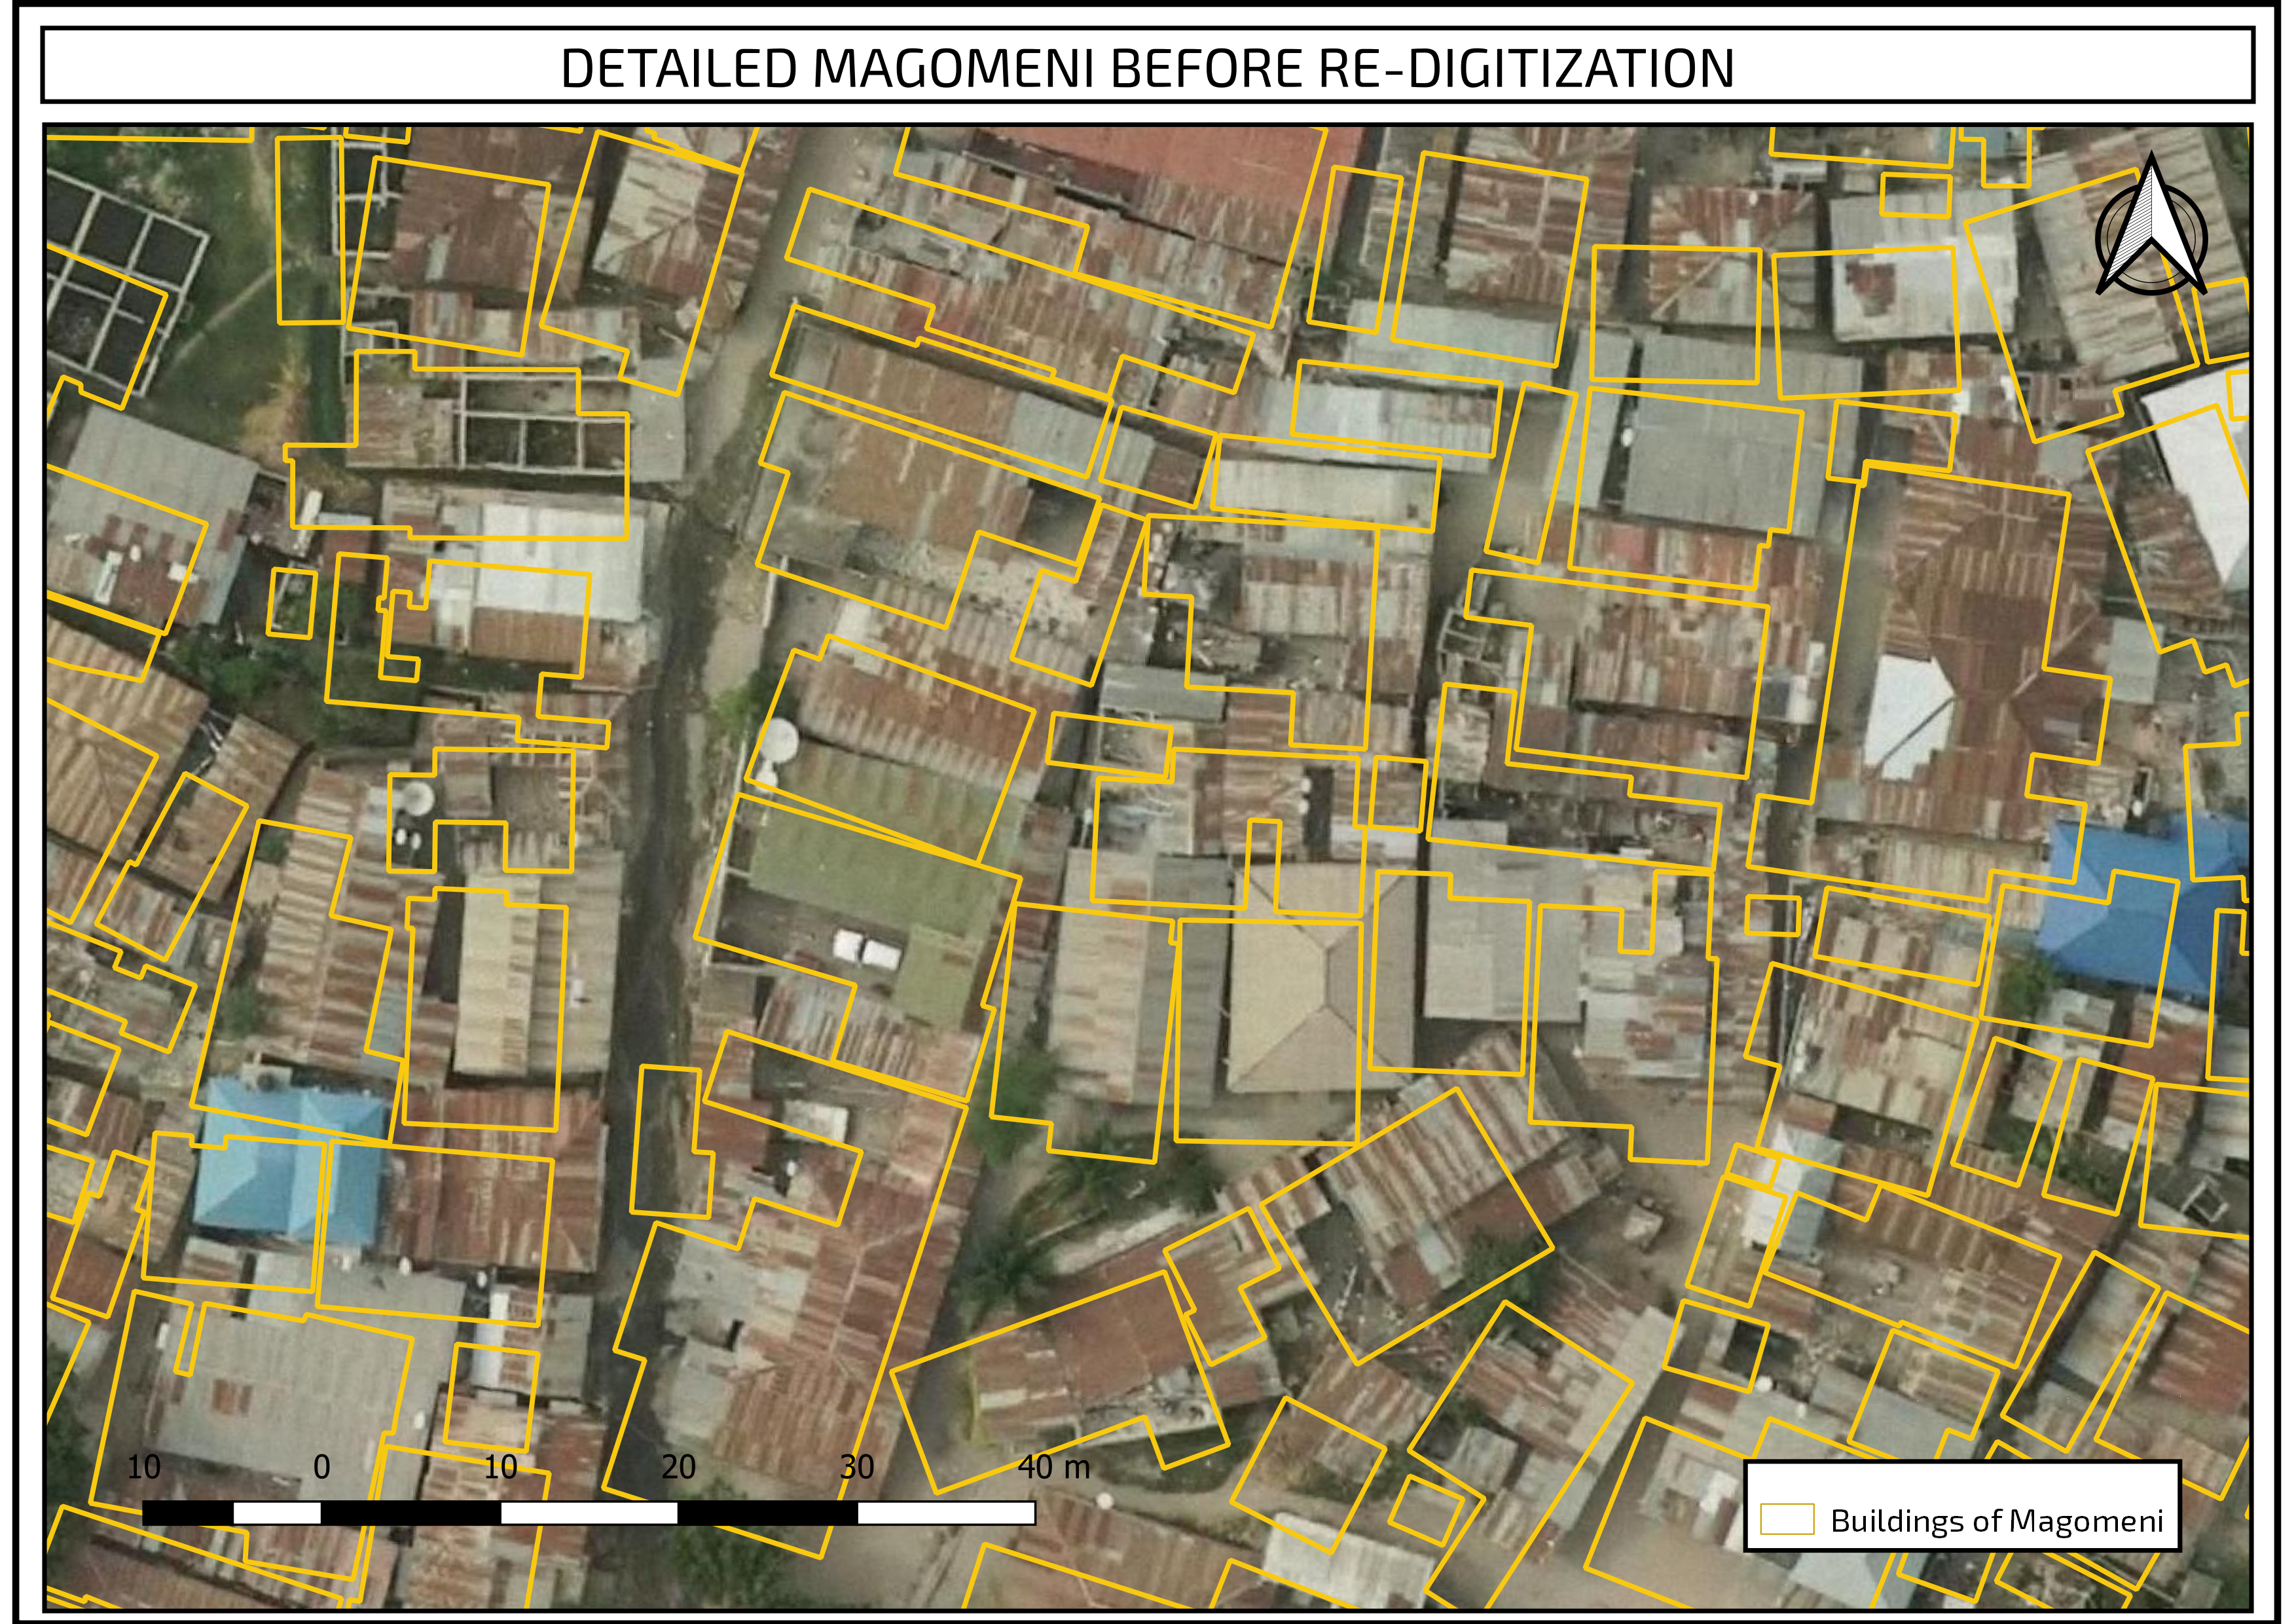
\includegraphics[width=\textwidth]{images/Detailed_Magomeni_Before_Redigitization.png}
   \color{RHgreen}\caption{Detailed image showing Magomeni ward before re-digitization using UAV imagery}
    \label{fig:1}
  \end{subfigure}
  %
  \begin{subfigure}[b]{0.5\textwidth}
    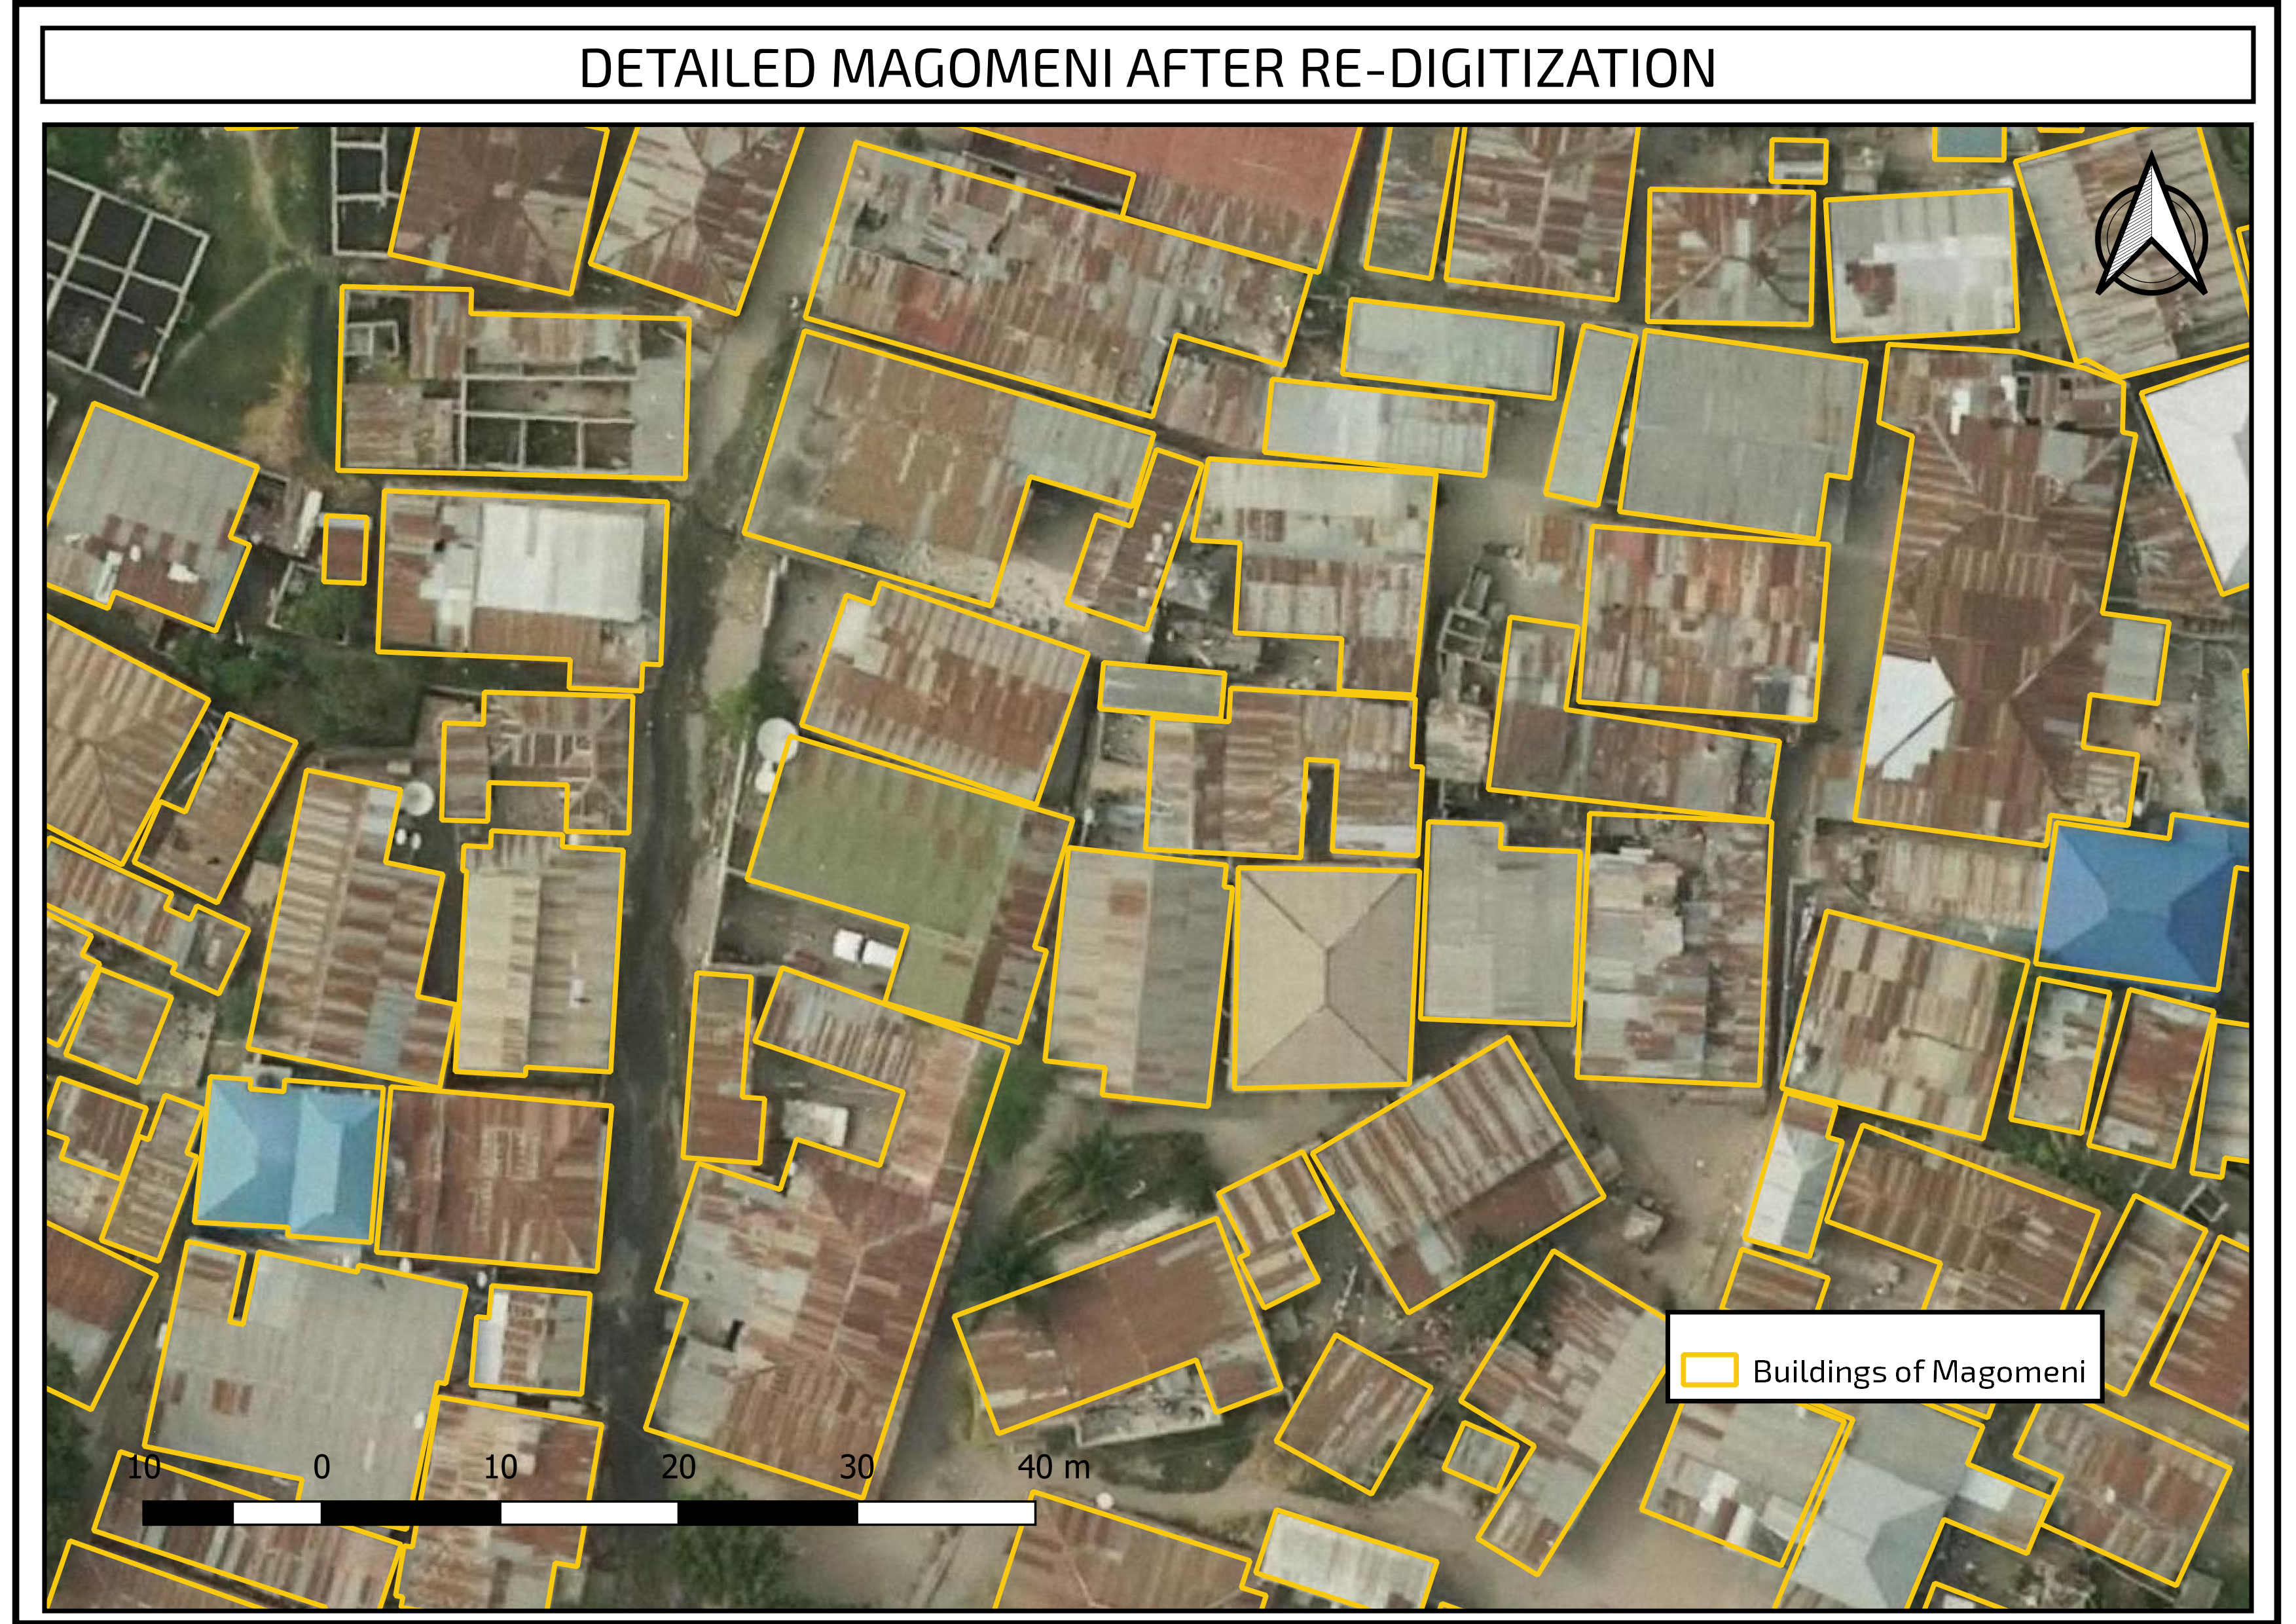
\includegraphics[width=\textwidth]{images/Detailed_Magomeni_After_Redigitization.png}
    \color{RHgreen}\caption{Detailed image showing Magomeni ward after re-digitization using UAV imagery}
    \label{fig:2}
  \end{subfigure}
\end{figure}

\subsubsection{Use Case}
Apart from showing how buildings are arranged, the digitized data has been used in other Ramani Huria activities such as Green WastePro and Assets and Threat Mapping.

\subsubsection{Data Gap}
Only 28 wards out of 44 Ramani Huria wards have been re-digitized by using high resolution imagery. There is a need to do the same for the remaining 20 Ramani Huria wards.
\subsubsection{Lessons Learned}
Dar es Salaam is a fast growing city and with that there are physical changes or development of the city in terms of buildings. New buildings are constructed and some are demolished from time to time therefore there is a need for re-digitization of the whole city.
\medskip

Re-digitization using a high quality imagery is important because the features can be seen clearly and it is difficult to miss any features when the image is clearer.

\newpage
\subsection{Administrative Divisions and Landmarks}
Hyperlocal boundaries are divisions within subwards regarded as political boundaries previously referred to as ten cell divisions as they were originally comprised of ten households.
Due to the increase in population, they comprise of 30 to 200 households and are administered by local leaders (wajumbe). Wajumbe are increasingly functioning as non-partisan public servants, often the first---in most cases---point of interaction between the government and citizens.
\medskip

Given the rate of urbanization in Dar es Salaam, it is very difficult to locate people and their respective addresses due to the unplanned and informal nature of these communities. Using more granular boundaries however makes it easier to locate people and provide services more precisely. 

\subsubsection{Spatial Extent}
36 out of 44 prioritized Ramani Huria wards in Dar es Salaam
\begin{figure}[h]
  \color{RHgreen}\caption{Map showing Ramani Huria collaboration with Data Zetu hyper-local boundaries mapping}
  \centering
  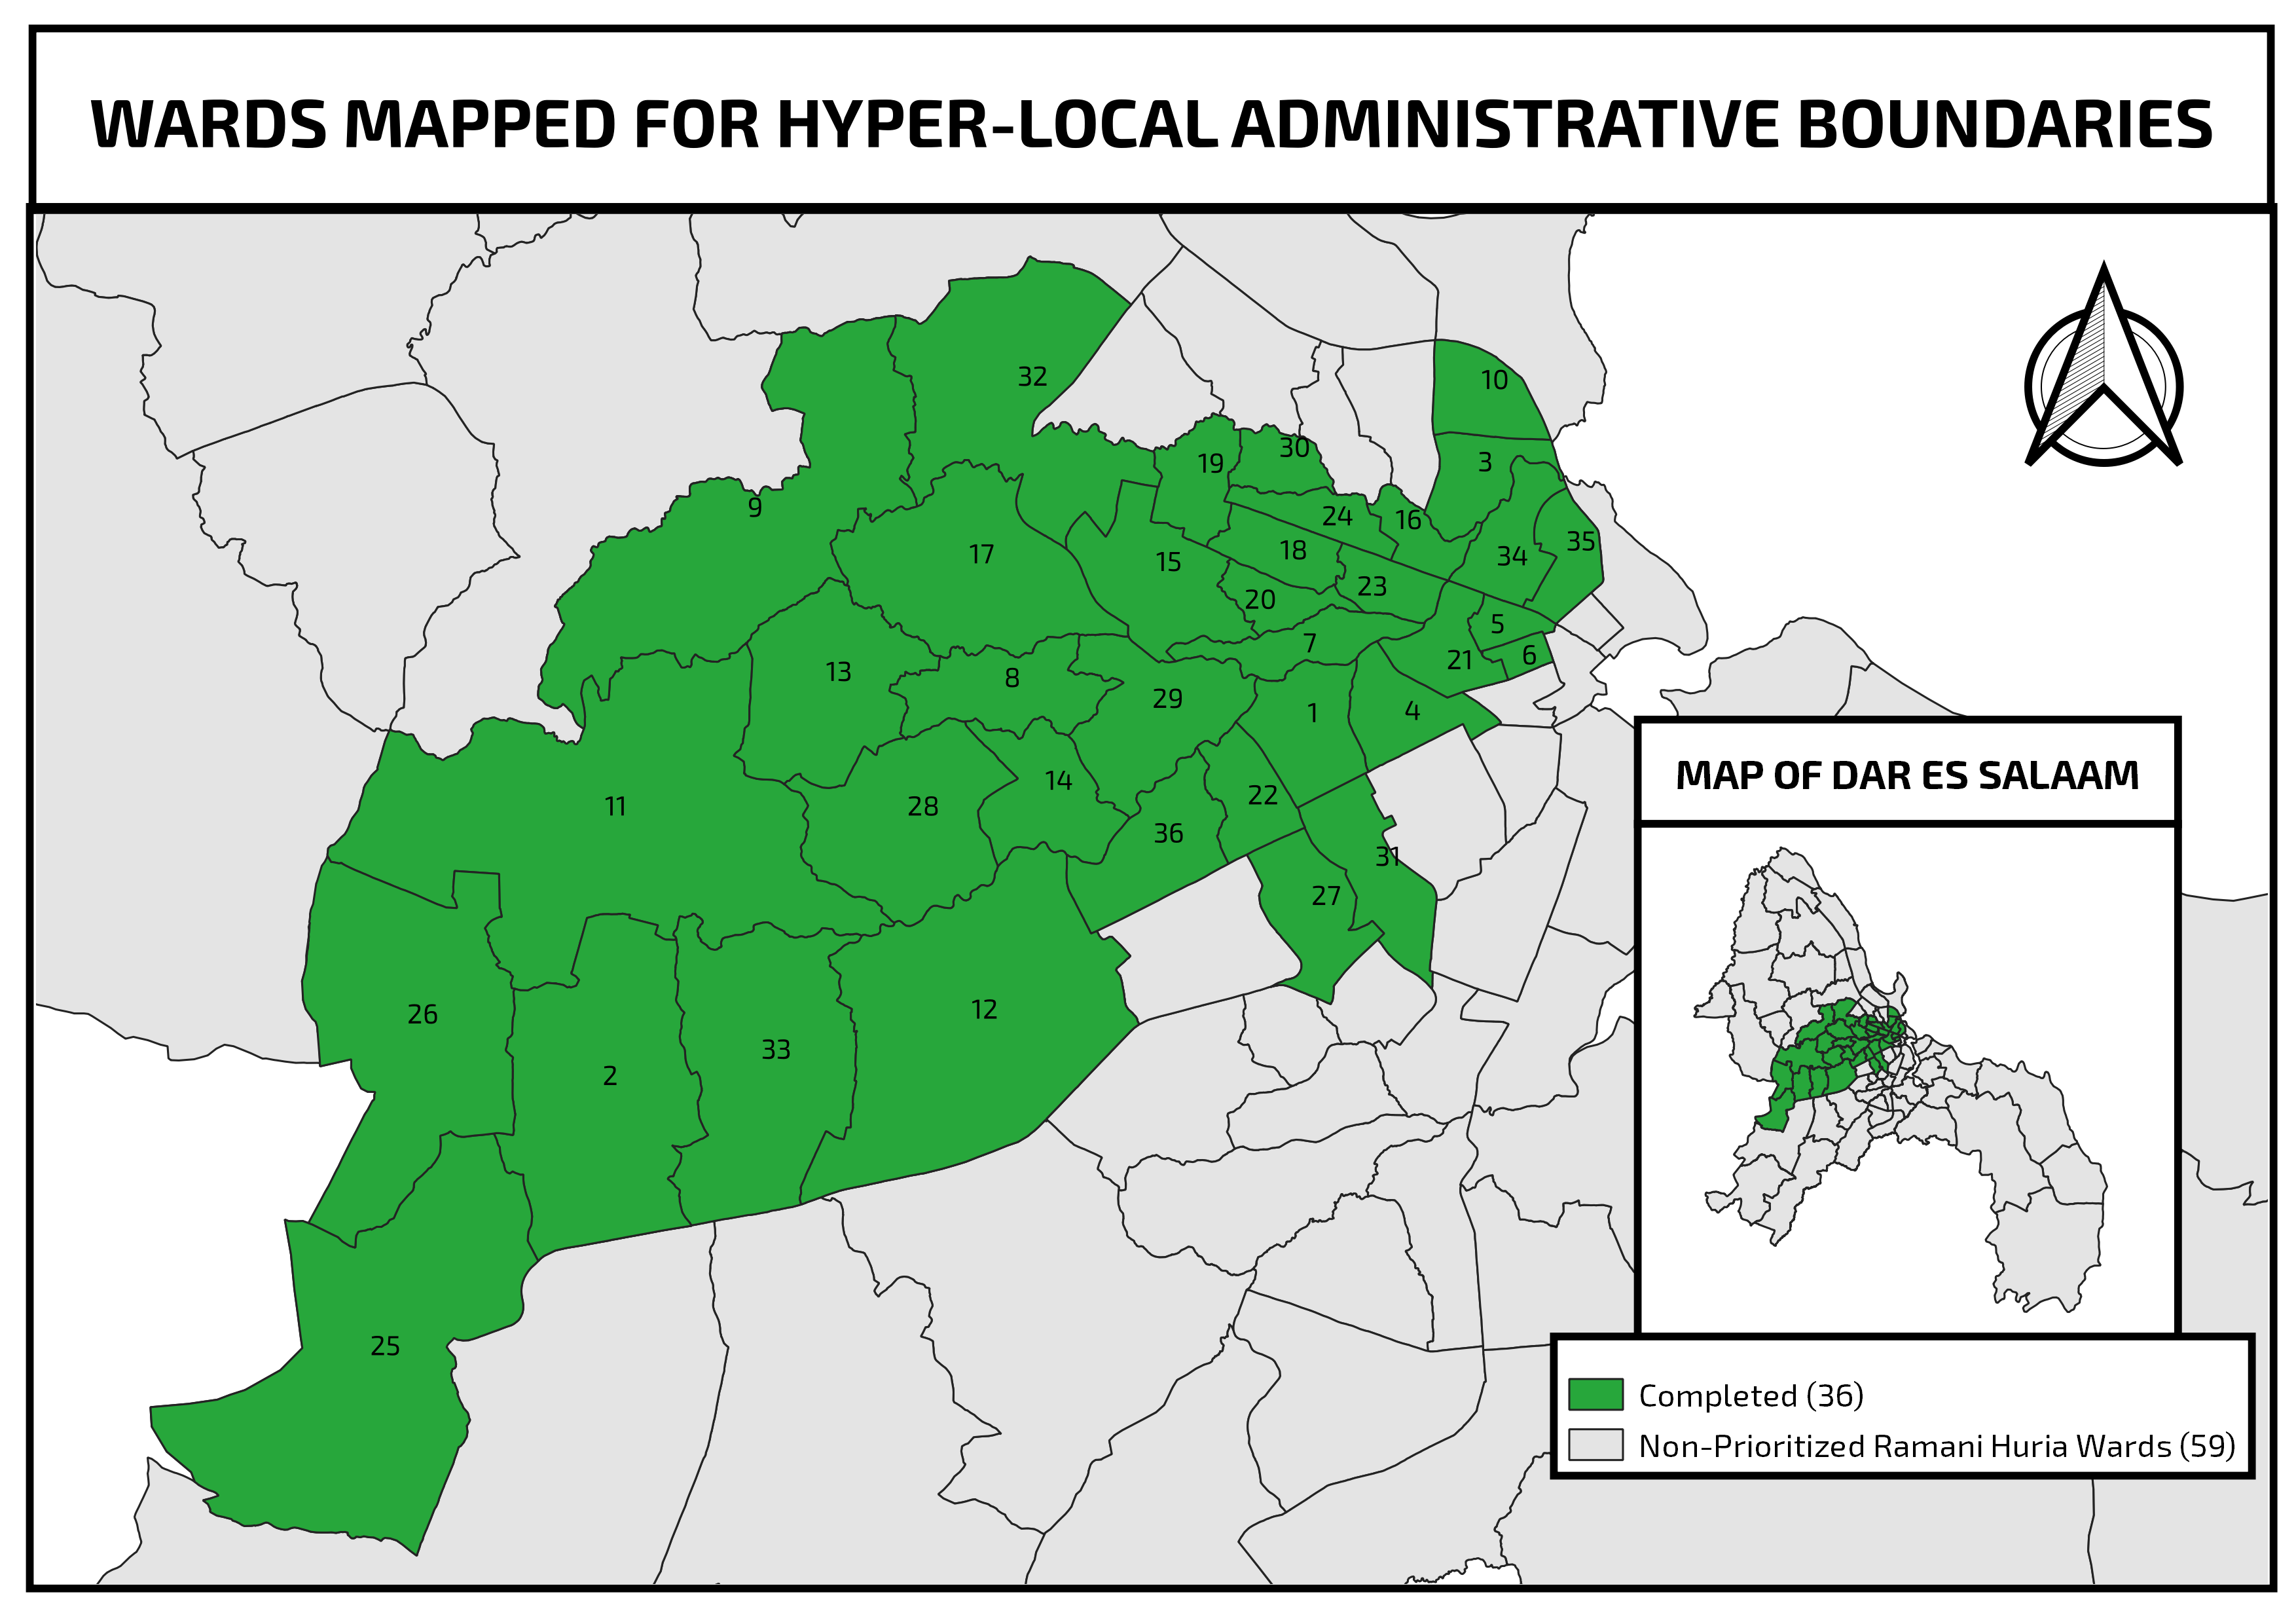
\includegraphics[width=0.8\textwidth]{images/hyperlocal_boundary.png}
\end{figure}



\subsubsection{Data Collection Methodology}
\begin{itemize}
    \item Introduction of the project from subward offices followed by training of selected community mappers on how to use ODK.
    \item Trained mappers work with wajumbe to trace their administrative boundaries. With assistance from supervisors, the collected data is checked and uploaded to the server. 
    \item Data cleaning was done using excel  and map creation using QGIS.
\end{itemize}

\subsubsection{Data Model}

\subsubsection{Timeline}
2018-09-13 to 2018-12-24

\subsubsection{Quality Assurance}
QGIS, Excel

\subsubsection{Access}
\href{https://drive.google.com/drive/u/1/folders/1bagTRoBVYX88VJpgYm61Rl2WXHgrvBJi}{Hyperlocal administrative boundary data}\footnote{\url{https://drive.google.com/drive/u/1/folders/1bagTRoBVYX88VJpgYm61Rl2WXHgrvBJi}}

\subsubsection{Licensing}
CC-BY 4.0

\subsubsection{Statistics}
2612 hyperlocal boundaries mapped in 36 wards of Dar es Salaam

\subsubsection{Data Visualization}

\subsubsection{Use Case}
To find people’s address in Dar es Salaam, \href{https://www.hotosm.org/updates/piloting-tanzanias-first-patient-origin-tracking-system/}{Amana Hospital patient origin tracking system}\footnote{\url{https://www.hotosm.org/updates/piloting-tanzanias-first-patient-origin-tracking-system/}}

\subsubsection{Data Gap}
All hyperlocal boundaries have been cleaned and verified for map production except Mabibo subward. The team faced political misunderstandings among wajumbe as most of the hyperlocal boundaries overlapped among different political parties and made it difficult for the team to trace the boundaries.

\subsubsection{Lesson Learned}
\begin{itemize}
    \item Overlaying of hyperlocal boundaries:
\end{itemize}
Some community leaders did not know their administrative boundaries which led to a number of buildings to fall in two or three different boundaries which made the data cleaning process very difficult.
\begin{itemize}
    \item Validation of cleaned data:
\end{itemize}
After identification of the problems, the team decided to validate the already cleaned data with local leaders in order to make sure that the errors are resolved. To ensure that this problem does not repeat itself, as soon as the community leaders finished tracing the boundaries, they worked with the supervisors to trace their boundaries on an A1 printed map with a satellite imagery to ensure data quality. 


\newpage
\subsection{Trash Mapping in Formal Settlements (Green WastePro Limited)}

Green WastePro Limited is a private company specialized in waste management with the aim to offer eco-friendly solutions in cleaning and waste management. They are mostly operate in formal settlements. The company needed digital methodology to obtain clients’ information including locations, clients contacts etc, so they can track clients and provide services accordingly.

\subsubsection{Spatial Extent}
\begin{figure}[h]
  \color{RHgreen}\caption{Map showing the mapped wards with GreenWaste Pro Limited}
  \centering
  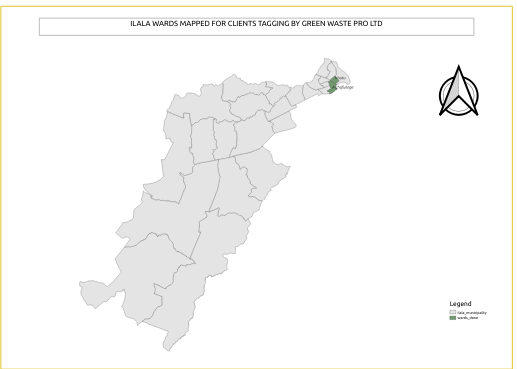
\includegraphics[width=0.8\textwidth]{images/GWPL_trial.png}
\end{figure}

\subsubsection{Methodology}
Collection of building data for each structure and resident/client data for each unit (residence or business) within the buildings in Kisutu and Mchafukoge wards in Dar es Salaam. Robust barcode stickers were placed at the entry of each unit, and a survey was completed for each unit where possible. The building data was uploaded to OSM, along with some amenity information gleaned from the unit surveys, and the remainder of the per-unit data was provided to GWPL.
\subsubsection{Data Model}
\subsubsection{Timeline}
October to November 2018
\subsubsection{Quality Control}
JOSM for buildings, QGIS for barcodes
\subsubsection{Access}
\href{https://drive.google.com/drive/u/1/folders/17DZDPi-_4FZlgXXd1qQ8deMHI57vdZcY}{GreenWaste Pro Limited data}\footnote{\url{https://drive.google.com/drive/u/1/folders/17DZDPi-_4FZlgXXd1qQ8deMHI57vdZcY}}
\subsubsection{Licensing}
CC-BY 4.0
\subsubsection{Statistics}
\subsubsection{Data Visualization}
\begin{figure}
  \begin{subfigure}[b]{0.4\textwidth}
    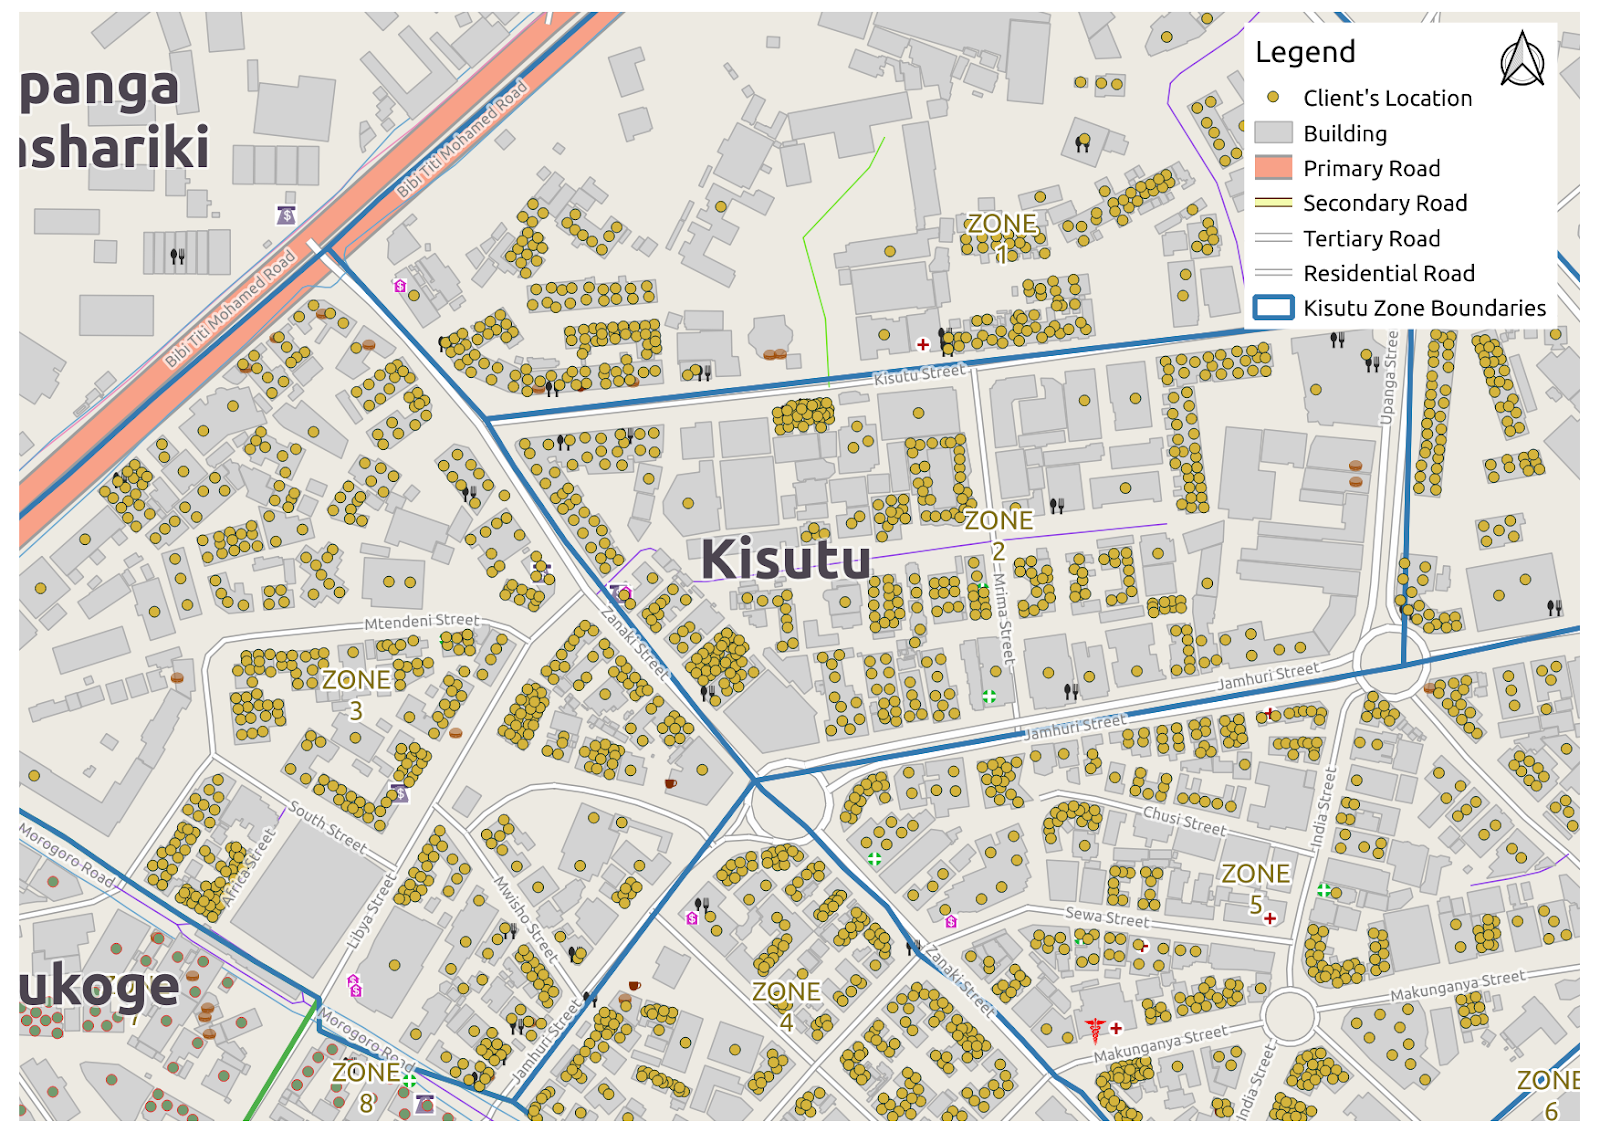
\includegraphics[width=\textwidth]{images/GWPL_client_map.png}
   \color{RHgreen}\caption{Map showing detailed collected points at Kisutu ward}
    \label{fig:1}
  \end{subfigure}
  %
  \begin{subfigure}[b]{0.5\textwidth}
    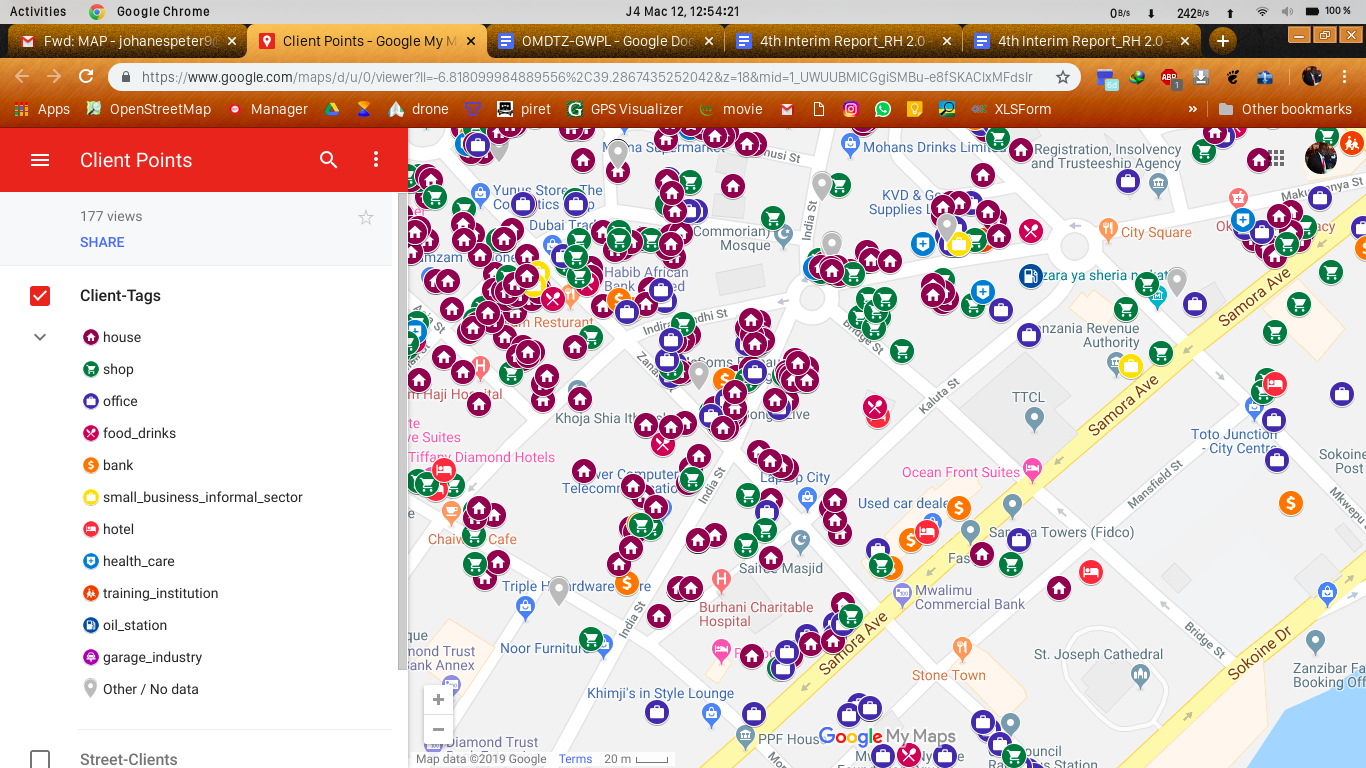
\includegraphics[width=\textwidth]{images/GWPL_client_tracking_system.png}
    \color{RHgreen}\caption{GWPL new client tracking system}
    \label{fig:2}
  \end{subfigure}
\end{figure}
\subsubsection{Use Case}
Creation of a client tracking system now used by GWPL to keep track of their clients
\subsubsection{Data Gaps}
Data was collected in only 2 wards of Dar es Salaam. The process needs to be replicated to other wards of the city
\subsubsection{Lessons Learned}

\newpage
\subsection{Trash Mapping in Informal Settlement (Joshemi Company Limited)}

Joshemi Company Limited (JCL) is a company entitled by the Ilala Municipal to collect solid waste in Tabata ward with eight subwards therein. The system of collecting waste and doing cleanliness within the company was done locally by revenue collectors to collect service charges from the customers by using local tools.

\subsubsection {Spatial Extent}
2 pilot subwards (Msimbazi Magharibi and Msimbazi Mama) out of eight subwards in Tabata ward.

\subsubsection{Methodology}
\begin{multicols}{2}
We used OpenDataKit (ODK) Collect and OpenMapKit (OMK) an extension of ODK which is a free and open android application for data collection. The team worked with revenue collectors to map the clients as they have a better understanding of the area to simplify the process of data collection. 

Ramani Huria team switched to working with local community leaders (wajumbe) who better understand their area of administration which normally ranges from 30 to 200 households. Among other things, wajumbe  are responsible for allocating resident leases and titles, therefore were able to provide clients’ details even when the clients were absent.

Tabata ward is 50\% informally developed hence most houses do not have house numbers. In order to connect the buildings’ geo locations with client information we developed “fake house ID” numbers as a baseline for the use of collected data.
\end{multicols}

\subsubsection{Data Model}

\subsubsection{Timeline}
November, 2018 to February, 2019

\subsubsection{Quality Control}
Google spreadsheet to fill in client information, JOSM for buildings, QGIS for client points

\subsubsection{Access}
\href{https://drive.google.com/drive/u/1/folders/1tUg6Tk2fQ4paIn-nQeUNFoQfmhkAaQYA}{Joshemi Company Limited (JCL) data}\footnote{\url{https://drive.google.com/drive/u/1/folders/1tUg6Tk2fQ4paIn-nQeUNFoQfmhkAaQYA}}

\subsubsection{Licensing}
CC-BY 4.0

\subsubsection{Statistics}
20163 trash points collected in 2 subwards of Tabata ward

\

\subsubsection{Data Visualization}
\begin{figure}
  \begin{subfigure}[b]{0.5\textwidth}
    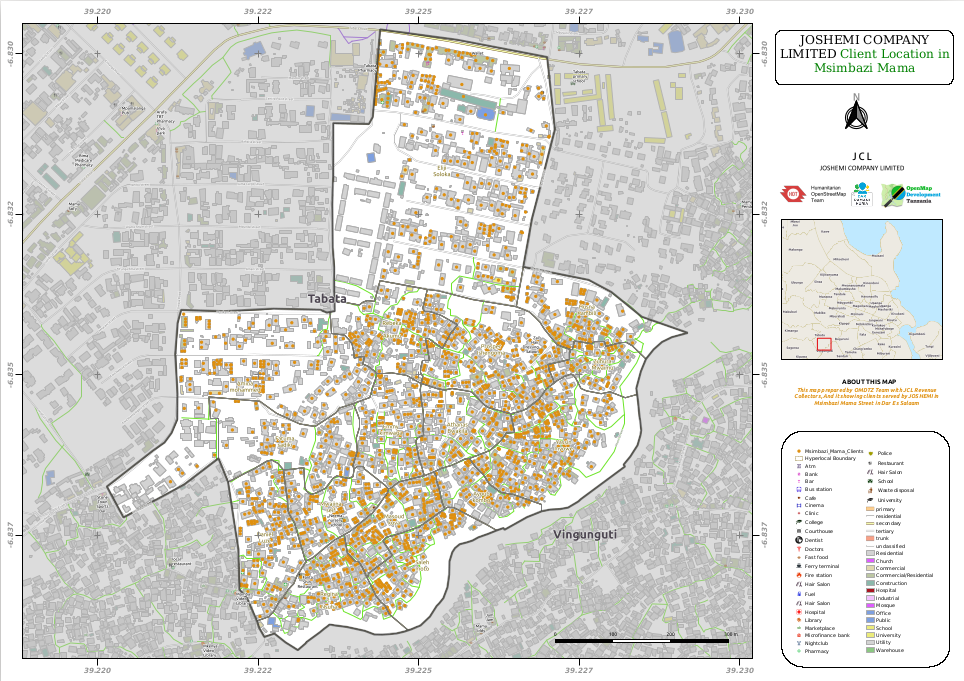
\includegraphics[width=\textwidth]{images/Msimbazi_mama.png}
   \color{RHgreen}\caption{A map showing client distribution, houses and hyperlocal boundaries in Msimbazi Mama}
    \label{fig:1}
  \end{subfigure}
  %
  \begin{subfigure}[b]{0.5\textwidth}
    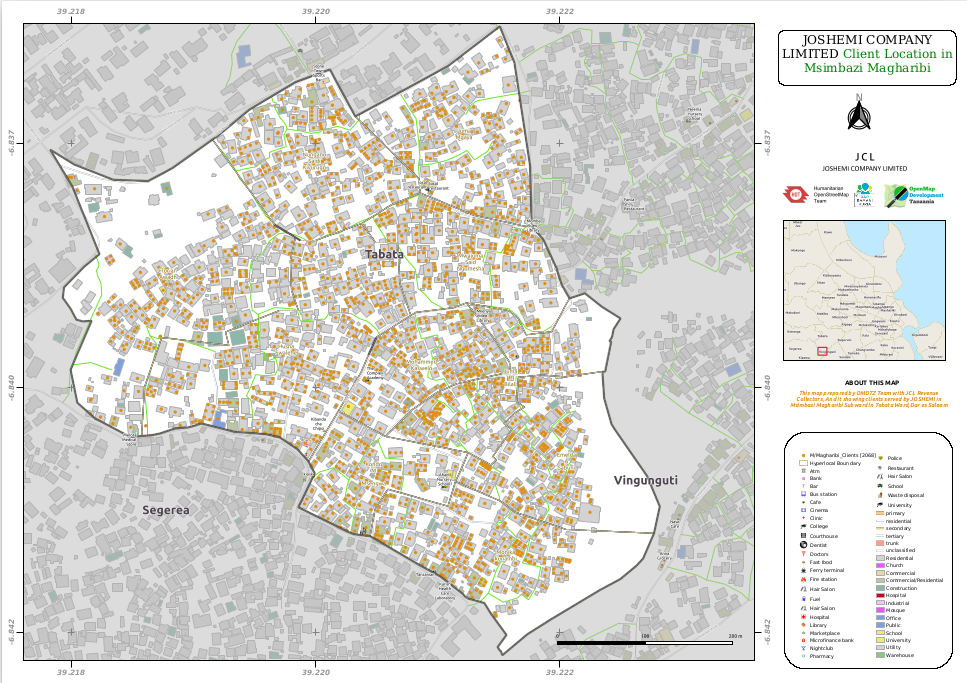
\includegraphics[width=\textwidth]{images/Msimbazi_magharibi.png}
    \color{RHgreen}\caption{Map showing client distribution, houses and hyperlocal boundaries in Msimbazi Magharibi}
    \label{fig:2}
  \end{subfigure}
\end{figure}

\subsubsection{Use Case}
The replication of the processes, system and using of trash dataset  in other wards & subwards to help  in the trash management. This can also reduce blockage of drains/waterways and hence make the ward flood resilient.

\subsubsection{Data Gap}
A system to collect  revenues and update clients who pay for the trash services has been created but the most hindrance is that, the personnel responsible to collect and use the system do not have/ own android smartphones---a requirement for data collection---and the company is hesitant to buy phones to be used by the revenue collectors.

\subsubsection{Lessons Learned}
\begin{itemize}
    \item There is a need to establish  a strong digital system of trash data collection to support companies and investors who are interested in waste management.
    \item There must be a channel that links the company to people so as to avoid challenges during data collection.
\end{itemize}

\newpage
\subsection{Dar es Salaam Trash Data}

A collaboration between Nipe Fagio (“give me the broom” in Swahili), a civil society organization founded in 2013 and Ramani Huria that joined forces and mapped trash sites in Dar es Salaam. The trash mapping initiative was part and parcel of the large Let’s-Do-It-World campaign, a civic-led mass movement to clean up countries.
\medskip

The mapped data helped to identify location of the areas with poorly managed waste materials, type and size of waste and clean up methods. This process helped ease cleaning the city on September 15th, 2018, a celebration of the world clean up day.

\subsubsection{Spatial Extent}
50 wards in Dar es Salaam

\subsubsection{Methodology}
Using OpenDataKit to collect trash points in the city and filling out the survey on the type of waste (debris, glass, metal), and the size of trash (hand full, bag full, truckload, cart etc) to ease cleaning process.
\medskip

Before field work, introduction letters were sent to ward officers so they can be informed and for mappers security in case there is any assistance needed from the ward office.

\subsubsection{Quality Assurance}
Some categories such as handful and bagful were far too small to be collected and sometimes confused the mappers therefore a decision to remove these points had to be made which dropped the number of points to approximately 9,000.

\subsubsection{Data Model}
\subsubsection{Timeline}
2018-07-30 to 2018-08-03

\subsubsection{Quality Control}
QGIS, data visualization tool

\subsubsection{Access}

\subsubsection{Licensing}
CC-BY 4.0

\subsubsection{Statistics}
A total of 20,392 points were collected and reduced to 9,452 after cleaning

\subsubsection{Data Visualization}
\begin{figure}[h]
  \color{RHgreen}\caption{Trash points collected during Dar es Salaam Trash Mapping}
  \centering
  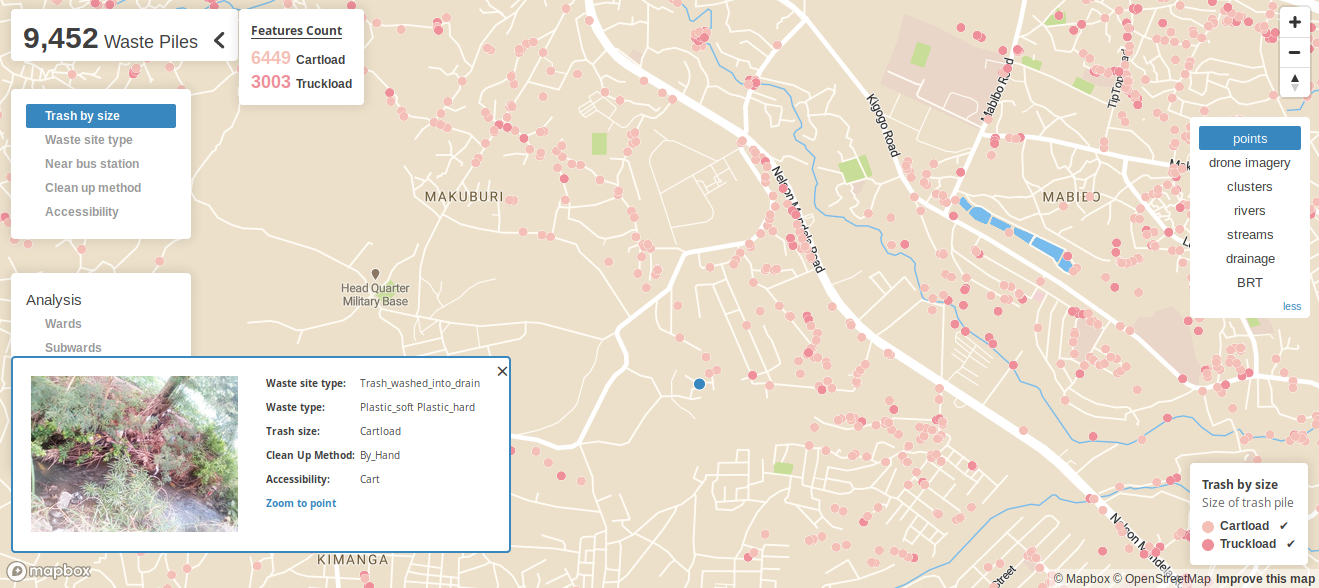
\includegraphics[width=0.8\textwidth]{images/dar_trash.png}
\end{figure}

\subsubsection{Use Case}
Data was used in the world clean up day on  September 15th, 2018 to help clean up the city.

\subsubsection{Data Gaps}
A decision to retain the data model used by the pioneers of the Clean Up the World Movement in Estonia was made since the model included the collection of waste piles as small as a handful or bagful, which in the context of Dar es Salaam was far too small and mappers possibly confused by the \textit{bagful} category in some cases collected the locations of waste which was bagged and prepared for pickup by waste disposal personnel. The removal of the two attributes dropped the number of trash points from 20,392 to 9,452.

\subsubsection{Lessons Learned}

\newpage
\subsection{Community Flood Response Mapping}
As a response to heavy rainfall on March, 3rd, 2019, that resulted in heavy flooding in some wards of Dar es Salaam, the Ramani Huria team decided to conduct field mapping to engage affected communities with the aim of \textit{conducting a rapid assessment and producing impact maps.}

\subsubsection{Spatial Extent}
3 majorly affected wards in Dar es Salaam with the March 3rd, 2019 rainfall

\begin{figure}[h]
  \color{RHgreen}\caption{Map showing the wards mapped during the March flood response}
  \centering
  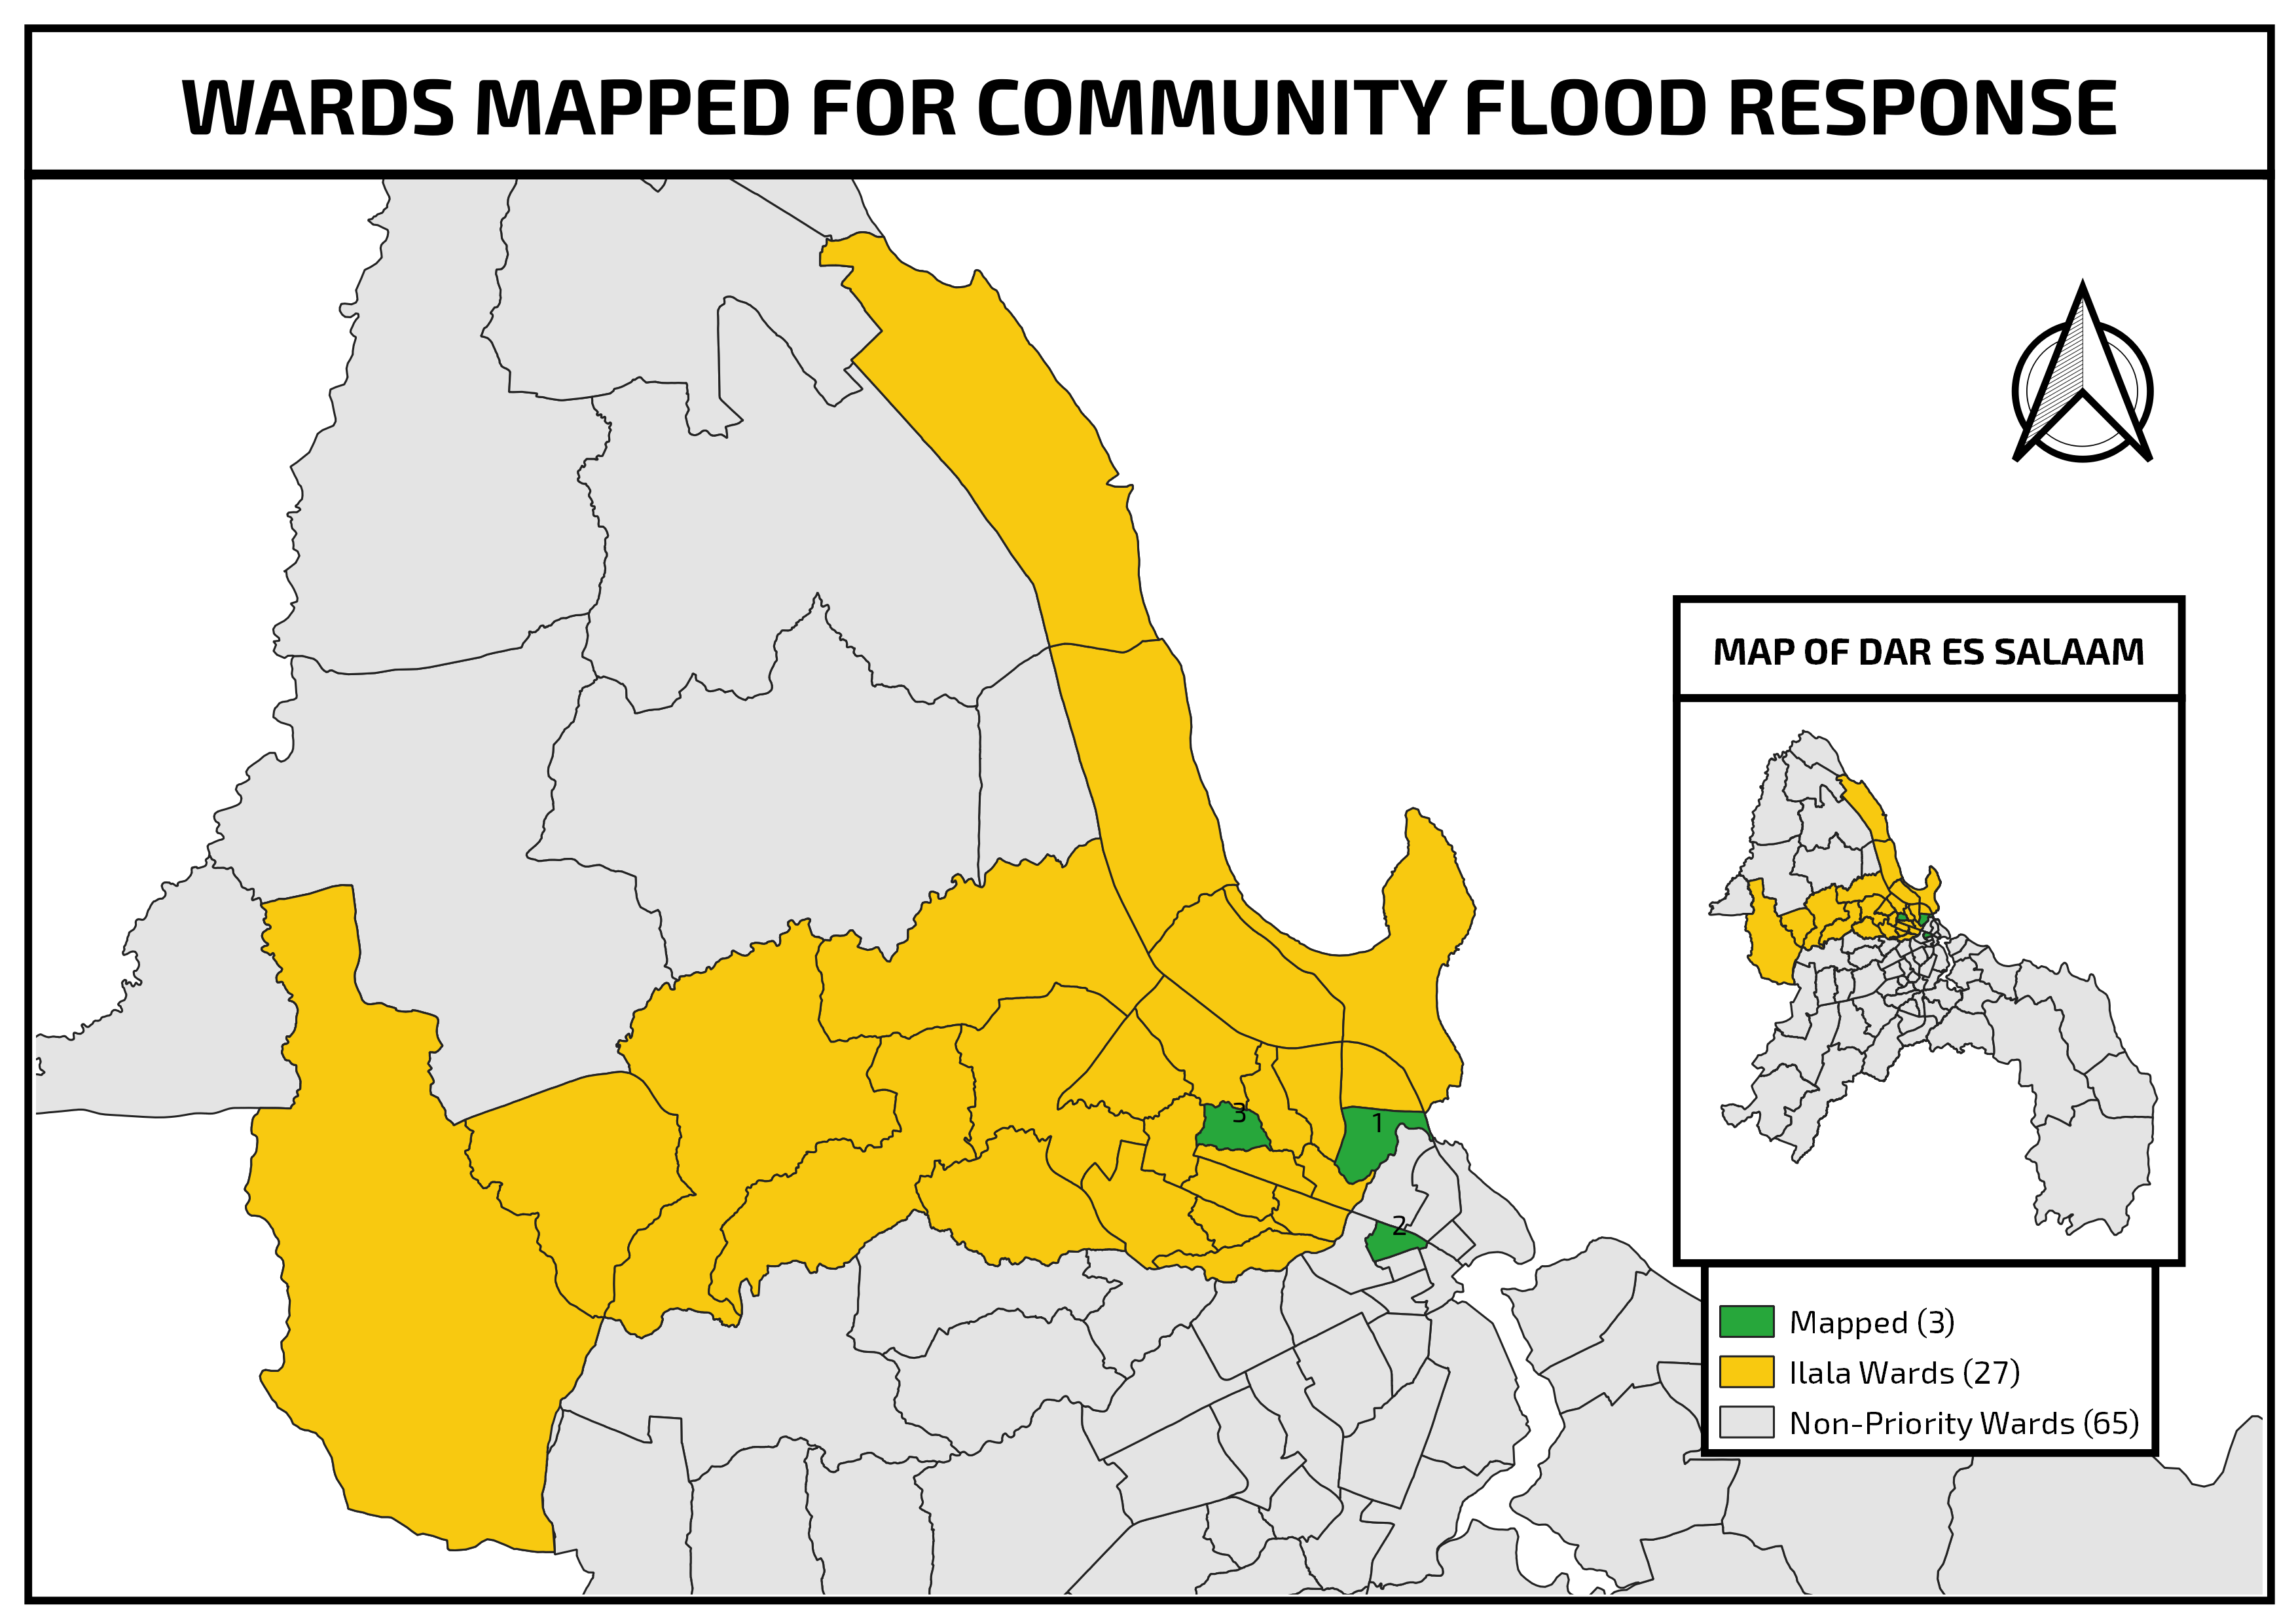
\includegraphics[width=0.8\textwidth]{images/flood_response.png}
\end{figure}

\subsubsection{Methodology}
Meetings with ward leaders in the three most affected subwards and zone the affected areas on a printed map with tracing paper and calculate the number of affected houses.

Field visit to survey the affected area and take points to verify what community leaders zoned on the map

\subsubsection{Data Model}
\subsubsection{Timeline}
2019-03-05

\subsubsection{Quality Control}
QGIS

\subsubsection{Access}
\href{https://drive.google.com/drive/u/1/folders/1Wmx3VyrHSpHmltPAF0RgfuO1mIrGyVI1}{Flood response mapping}\footnote{\url{https://drive.google.com/drive/u/1/folders/1Wmx3VyrHSpHmltPAF0RgfuO1mIrGyVI1}}

\subsubsection{Licensing}
CC-BY 4.0

\subsubsection{Statistics}
\begin{center}
\begin{tabular}{|c|c|c|c|}
\hline
Ward & Subward & Total number of houses flooded \\
\hline
Hannanasifu & Mkunguni B & 150 houses \\
\hline
Tandale & Mkunduge & 1100 houses \\
\hline
Tandale & Sokoni & 230 houses \\
\hline
Jangwani & Mtambani & 427 houses \\
\hline
\end{tabular}
\end{center}

\subsubsection{Data Visualization}

\subsubsection{Use Case}
To extract some types of information which are otherwise difficult to access by traditional methods, particularly for flood forecasting and flood water movement through identifying the affected areas and causative.
Conducting damage assessment of the affected areas.

\subsubsection{Data Gaps}
We did  community flood response for only 3 wards which were affected with flood but were not able to visit other wards which were also affected.

\subsubsection{Lessons Learned}
\begin{enumerate}
    \item The team was  not prepared for the incidence because we never did flood response before. Therefore when it happened we did not have tools and a proper methodology to conduct the survey which includes going  directly to the flooded area.
    \item Due to poor accessibility to the flooded area, we collected flood response points with help from local leaders/ wajumbe who know to  what extent the rains affected people’s houses. This information, however, might not be 100\% correct.
\end{enumerate}
\medskip

As a humanitarian organization dealing with disaster response, we should always be prepared to respond to such disasters on time and without delay---all tools and equipment must be set prior the event.

\newpage
\subsection{Historical Flood Extents}

Historical flood extent covered areas that are mostly affected by floods during rainy seasons. Households surveys were conducted to capture details in  subwards of the respective wards across the Msimbazi River rivers and streams that outflow to the main river.

\medskip

The information captured aimed to know whether the respondent had been affected by floods in the previous years, the flood depth and flood occurrence years---historical flood events. Individuals were asked to reflect on historical flood extents; therefore there is inherent subjectivity in their memories

\subsubsection{Spatial Extent}
\begin{figure}[h]
  \color{RHgreen}\caption{Map showing the flood extent mapping progress in Dar es Salaam}
  \centering
  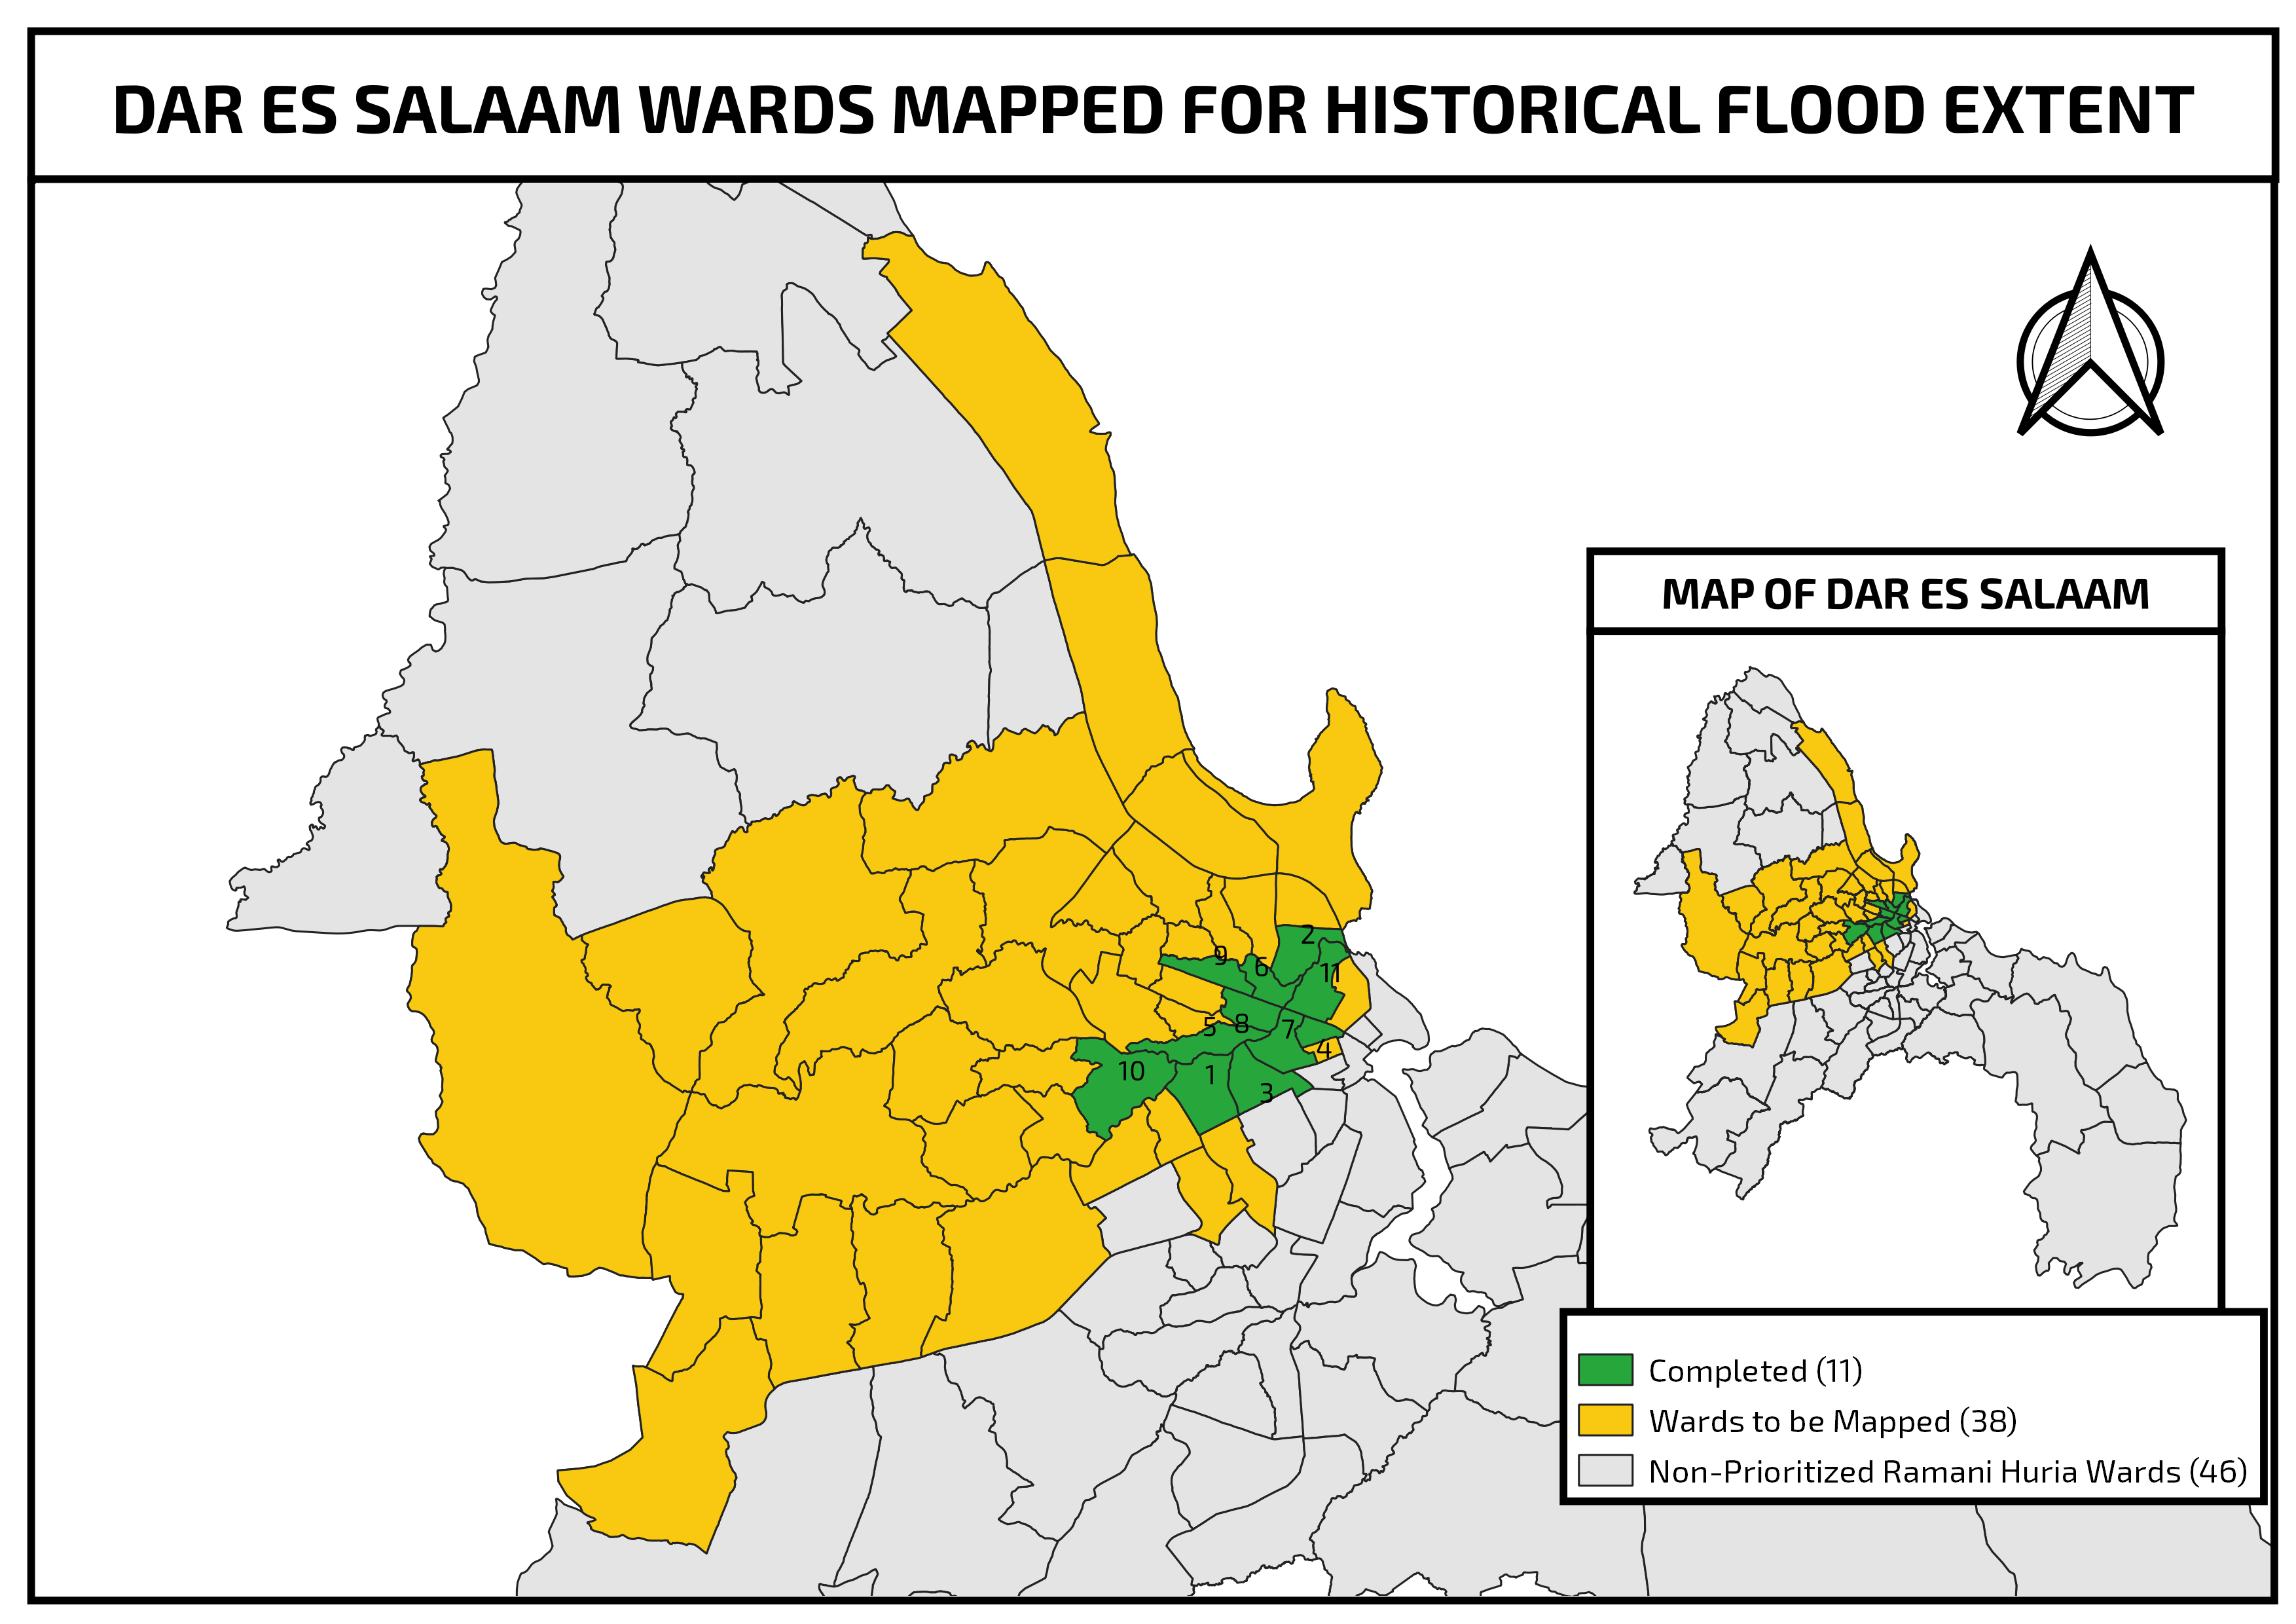
\includegraphics[width=0.8\textwidth]{Flood_Extent.png}
\end{figure}


\subsubsection{Data Collection Methodology}
Using ODK survey form and asking questions to community members about their experience of floods in their neighbourhoods. Community members of the respective wards were trained on how to collect data using ODK and were the ones to collect these information in their own neighborhood.

\subsubsection{Data Model}

\subsubsection{Timeline}
2017-08-24 to 2018-04-12

\subsubsection{Quality Assurance}
QGIS, Excel

\subsubsection{Access}
\begin{itemize}
    \item \href{https://drive.google.com/drive/u/1/folders/1F8P8A5tmxnC8pth4ZDrR6G_OwHF0rV5k}{Historical flood extent data}\footnote{\url{https://drive.google.com/drive/u/1/folders/1F8P8A5tmxnC8pth4ZDrR6G_OwHF0rV5k}}
    \item \href{http://geonode.uhurulabs.org/layers/geonode\%3Adar_flood_depths#more}{Dar es Salaam Flood Survey}\footnote{\url{http://geonode.uhurulabs.org/layers/geonode\%3Adar_flood_depths#more}}
    \item \href{http://geonode.uhurulabs.org/layers/geonode\%3Adar_flood_depths#more}{Dar es Salaam Flood Depths}\footnote{\url{http://geonode.uhurulabs.org/layers/geonode\%3Adar_flood_depths#more}}
\end{itemize}

\subsubsection{Licensing}
CC-BY 4.0

\subsubsection{Statistics}
Approximately 30 000 houses were surveyed during the historical flood extents


\subsubsection{Data Visualization}

\subsubsection{Use Case}
Designing of the lower Msimbazi River catchment area, data is used to understand the extent to which houses are affected from Msimbazi valley.

\subsubsection{Data Gap}
Individuals were asked to reflect on historical flood extents; therefore there is inherent subjectivity in their memories

\subsubsection{Lessons Learned}
Being keen while working with community members i.e. they did not know units of measurements. In some of their responses, they estimated flood depth as 100 meters which was practically impossible.
The team had to re-design the ODK form to make it simple when community members estimate the depth of floods by using man’s height i.e. knee deep, chest deep, waist deep etc.


\newpage
\section{Annexes}


\end{document}